% Overrides original definition
\def\rmhtmet{\mbox{$\mathcal{R}$}\xspace}

%%____________________________________________________________________________||
\newpage
\section{Background estimation for QCD multijet events \label{sec:qcd}}

One of the major challenges for searches of new physics in the jets +
\met final state is the control of background events from QCD multijet
production. The difficulties in the determination of precise estimates
for this background stem from the large cross sections expected in the
high-energy, high-luminosity hadron collider environment at the LHC,
which are further compounded by the lack of precise theoretical
predictions for the cross sections and kinematic properties of
multijet events. Hence, without special consideration and treatment,
significant uncertainties on large background expectations can
overwhelm any potential sensitivity to new physics signatures.

With regards to QCD multijet production, the approach of this search
is to favour the suppression of the multijet background to a
negligible level over the goal of high efficiency for any given signal
model. A conservative uncertainty on a negligible contribution is
preferred over a procedure that attempts to accurately estimate a
non-negligible contribution from multijet events. The level of
contamination should be sufficiently small (\ie sub-percent level)
such that the associated uncertainty, even if large, will be
sub-dominant with respect to the uncertainties on the remaining SM
backgrounds with genuine \met such as \wj, \znunu, and \ttbar,
henceforth labelled as non-multijet processes.

Any contamination from QCD multijet events is controlled primarily
through the \alphat and \bdphi variables. The \alphat variable,
described in Section~\ref{sec:alphatdef}, is able to distinguish with
high efficiency the sources of ``fake'' \met, such as jet energy
mismeasurement, from those with ``genuine'' \met, such as neutrinos.
The \bdphi variable, described in Section~\ref{sec:bdphi-selection},
is also very efficient at identifying jets that suffer
under-measurements, as well as over-measurements, in (otherwise
balanced) multijet events. The variable is also particularly suited to
identifying multijet events that exhibit significant \met due to the
production of neutrinos (collinear with a jet axis) in semileptonic
heavy-flavour decays. Both variables are individually capable of
reducing the yields from multijet events by several orders of
magnitude, and combined provide an extremely robust method to reject
multijet events. Figure~\ref{fig:alphat_bdphi_distr} shows the
distributions in data for the \alphat and \bdphi variables.

\begin{figure}[!t]
 \centering
 \subfigure[\bdphi distribution.\label{fig:alphat_distr}]{
 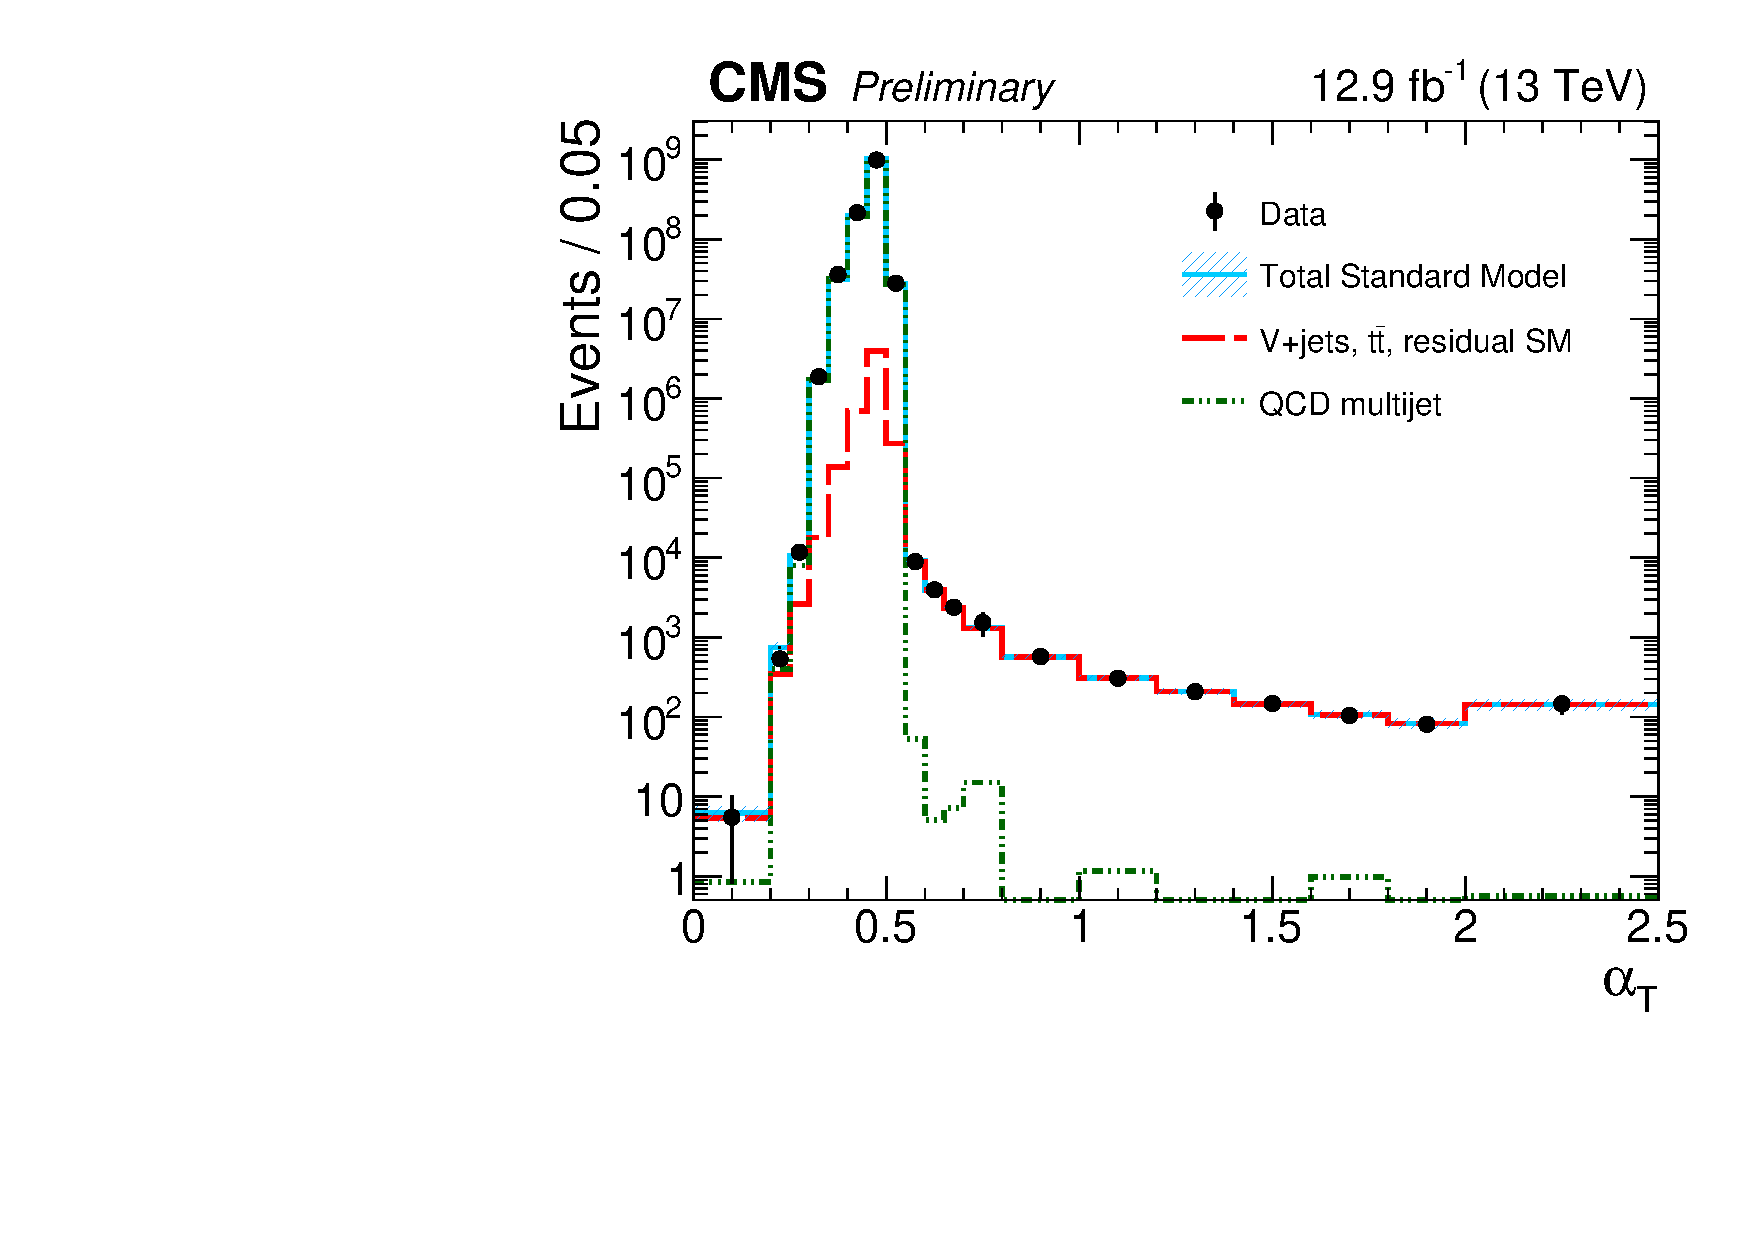
\includegraphics[width=0.5\textwidth]{figures/qcd/CMS-PAS-SUS-16-016_Figure-aux_001.pdf}
 }
 \subfigure[\dphimhtj distribution.\label{fig:bdphi_distr}]{
 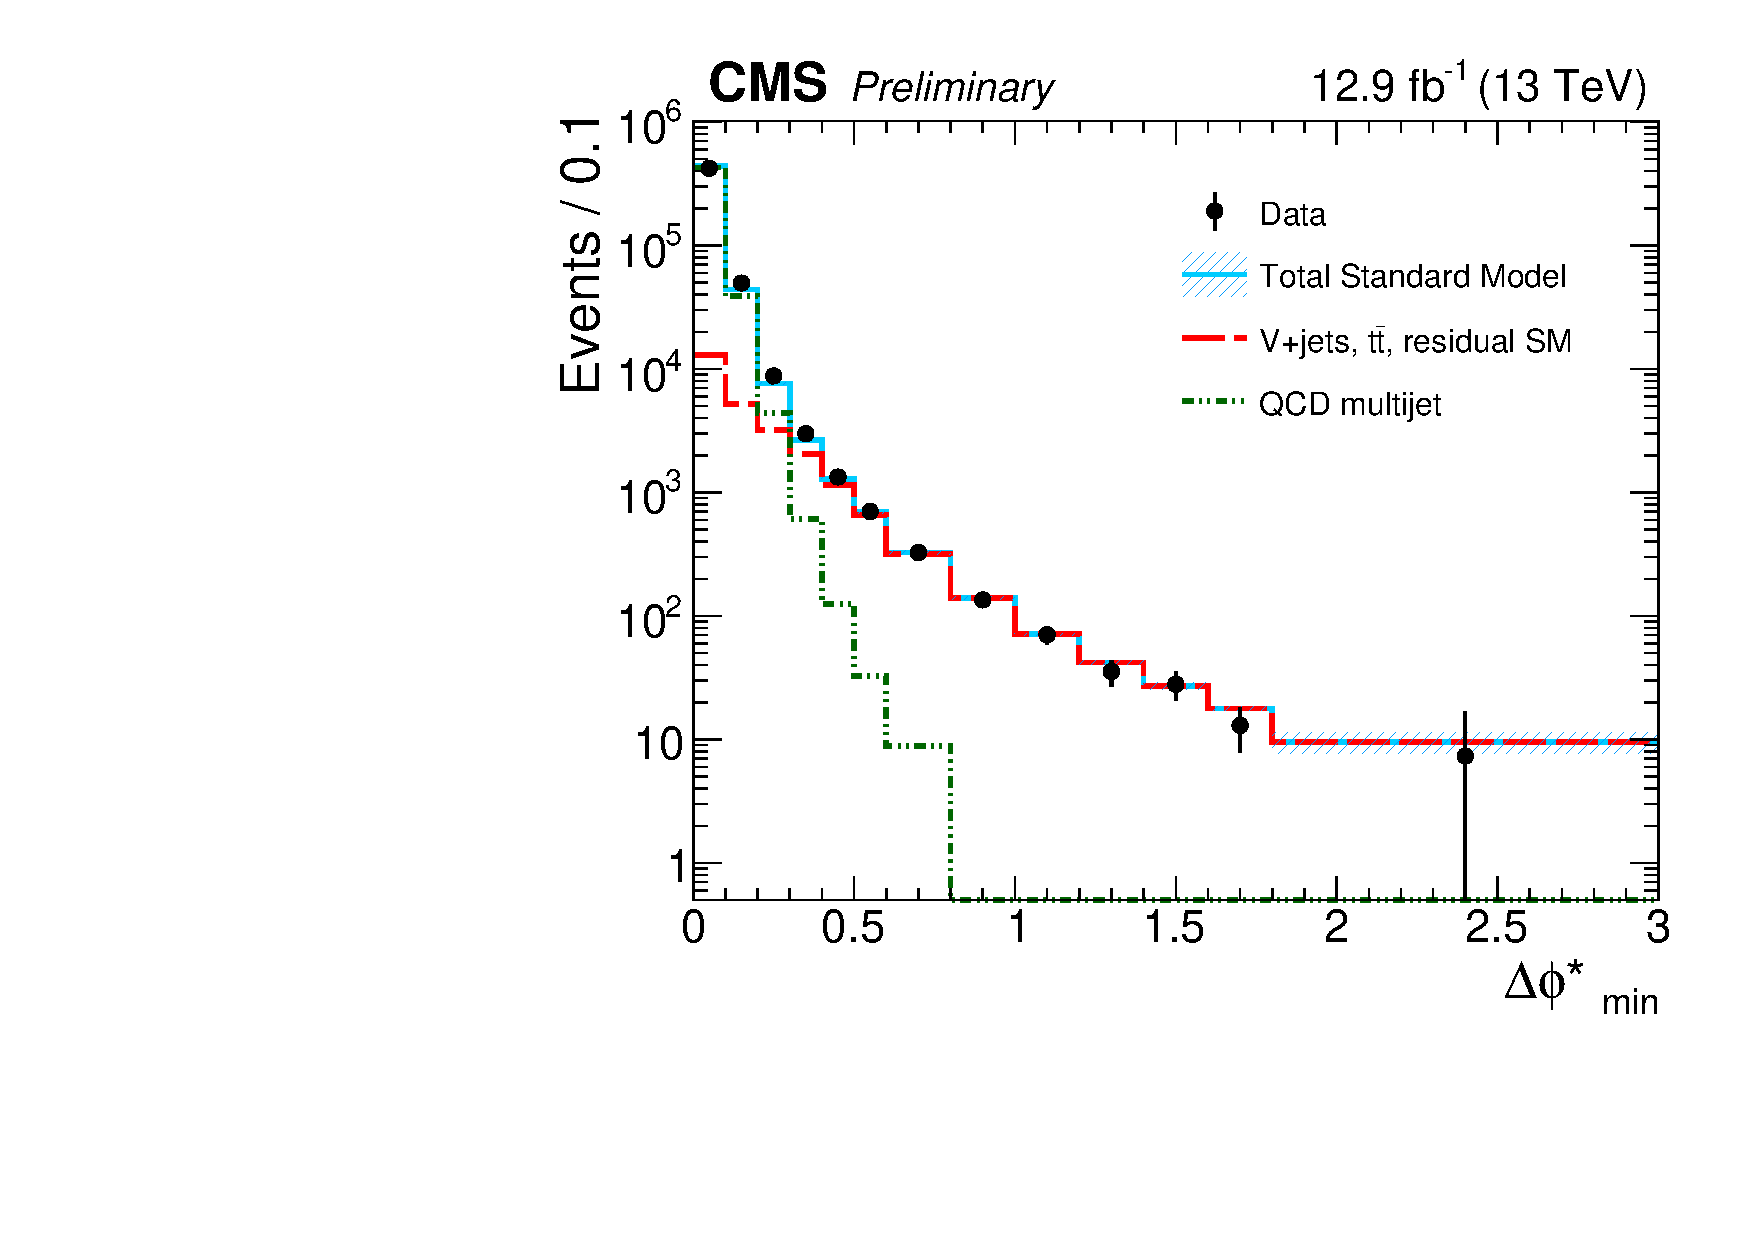
\includegraphics[width=0.5\textwidth]{figures/qcd/CMS-PAS-SUS-16-016_Figure-aux_002.pdf}
 } \\
 \caption{(Left) The \alphat distribution in data for events
   satisfying the pre-selection criteria when $\alphat < 0.55$ and the
   full signal selection criteria when $\alphat > 0.55$. (Right) The
   \bdphi distribution in data for events satisfying the pre-selection
   criteria and $\scalht > 800\GeV$. \fixme{Needs updating to the full
     data set.}
 }
 \label{fig:alphat_bdphi_distr}
\end{figure}

\subsection{The method}
\label{sec:qcdMethod}

Potential contamination from multijet events in the signal region is
estimated by exploiting the ratio $\rmhtmet$ of multijet events that
satisfy or fail the requirement $\mht/\met < 1.25$, as determined from
simulation, for events categorised according to \njet and
\scalht. Estimates of the QCD multijet background counts are
determined in a data sideband, defined by the requirement $1.25 <
\mht/\met < 3.0$, by correcting the observed counts in data to account
for contamination from non-multijet backgrounds (vector boson and
\ttbar production, plus residual contributions from other SM
processes), henceforth in this section collectively labelled as the
``EWK'' backgrounds. The products of the corrected counts and ratios
provide independent estimates of the multijet background as a function
of \njet and \scalht.

A binned maximum-likelihood fit to data counts in the sideband,
analagous to that described in Sec.~\ref{sec:likelihood}, is performed
to obtain an estimate of the number of QCD multijet events in each
(\njet, \scalht) bin of the sideband region. The sideband data are
collected with a logical \verb!OR!  of the ``monojet'',
\verb!HLT_HTxxx_AlphaT0pyy!, and \verb!HLT_HT800!  signal triggers,
described in Sec.~\ref{sec:triggers}.

The sideband is enriched in QCD multijet events, but the contribution
from EWK backgrounds can be sizeable and must be accounted for. The
EWK backgrounds are estimated with the ``transfer method'', described
in Sec.~\ref{sec:ewk-method}, using the single muon, double muon and
single photon control regions. These regions are defined by the same
selection criteria described in Sec.~\ref{sec:selection}, except for
the inverted requirement on \mhtmet. All relevant systematic
uncertainties in the EWK background estimates are taken into account,
including the sources of experimental uncertainties described in
Sec.~\ref{sec:mc-variations} and the data-driven uncertainties
determined from ``closure tests'', described in
Sec.~\ref{sec:closure-tests}. The fit to data assumes only the
presence of QCD and EWK contributions. Signal contamination is
expected to be negligible. A floating parameter per (\njet, \scalht)
bin is assigned as a multiplier (``signal strength'') term,
$\mu_{\textrm{QCD}}$, on the QCD expectation from simulation. The fit
is used to constrain these floating parameters, which are then used to
``correct'' the raw counts from the simulation in order to provide an
accurate estimate of the QCD counts ($\mathcal{Q}$) in each bin of the
sideband. The products of these predicted QCD counts and the ratio,
$\mathcal{Q} \times \rmhtmet$, provide an estimate of the level of QCD
multijet events in each (\njet, \scalht) bin of the signal region.

Figure~\ref{fig:mhtmet_sideband} summarises the observed data counts,
post-fit estimates of the EWK and QCD background contributions, and
the constrained values of the floating parameters
$\mu_{\textrm{QCD}}$, as a function of \njet and \scalht in the
\mhtmet sideband. Pre-fit QCD values are not shown, but can be
inferred from the post-fit and $\mu_{\textrm{QCD}}$ values. 

Figure~\ref{fig:qcd_estimate} summarises the pass/fail ratios
\rmhtmet, the EWK and QCD background predictions, and the ratios of
QCD/EWK predictions in the (\njet, \scalht) bins of the signal
region. The QCD background estimates are typically very small, and
below the percent level with respect to the total non-multijet
backgrounds. This level of suppression is compatible with the levels
seen for pervious iterations of this search, at both $\sqrt{s} = 8$
and 13\TeV. The predicted multijet event counts are included as a
background contribution to the likelihood model, described in
Sec~\ref{sec:likelihood}.

\clearpage
\begin{figure}[!t]
  \centering
  \subfigure[Data counts.]{
    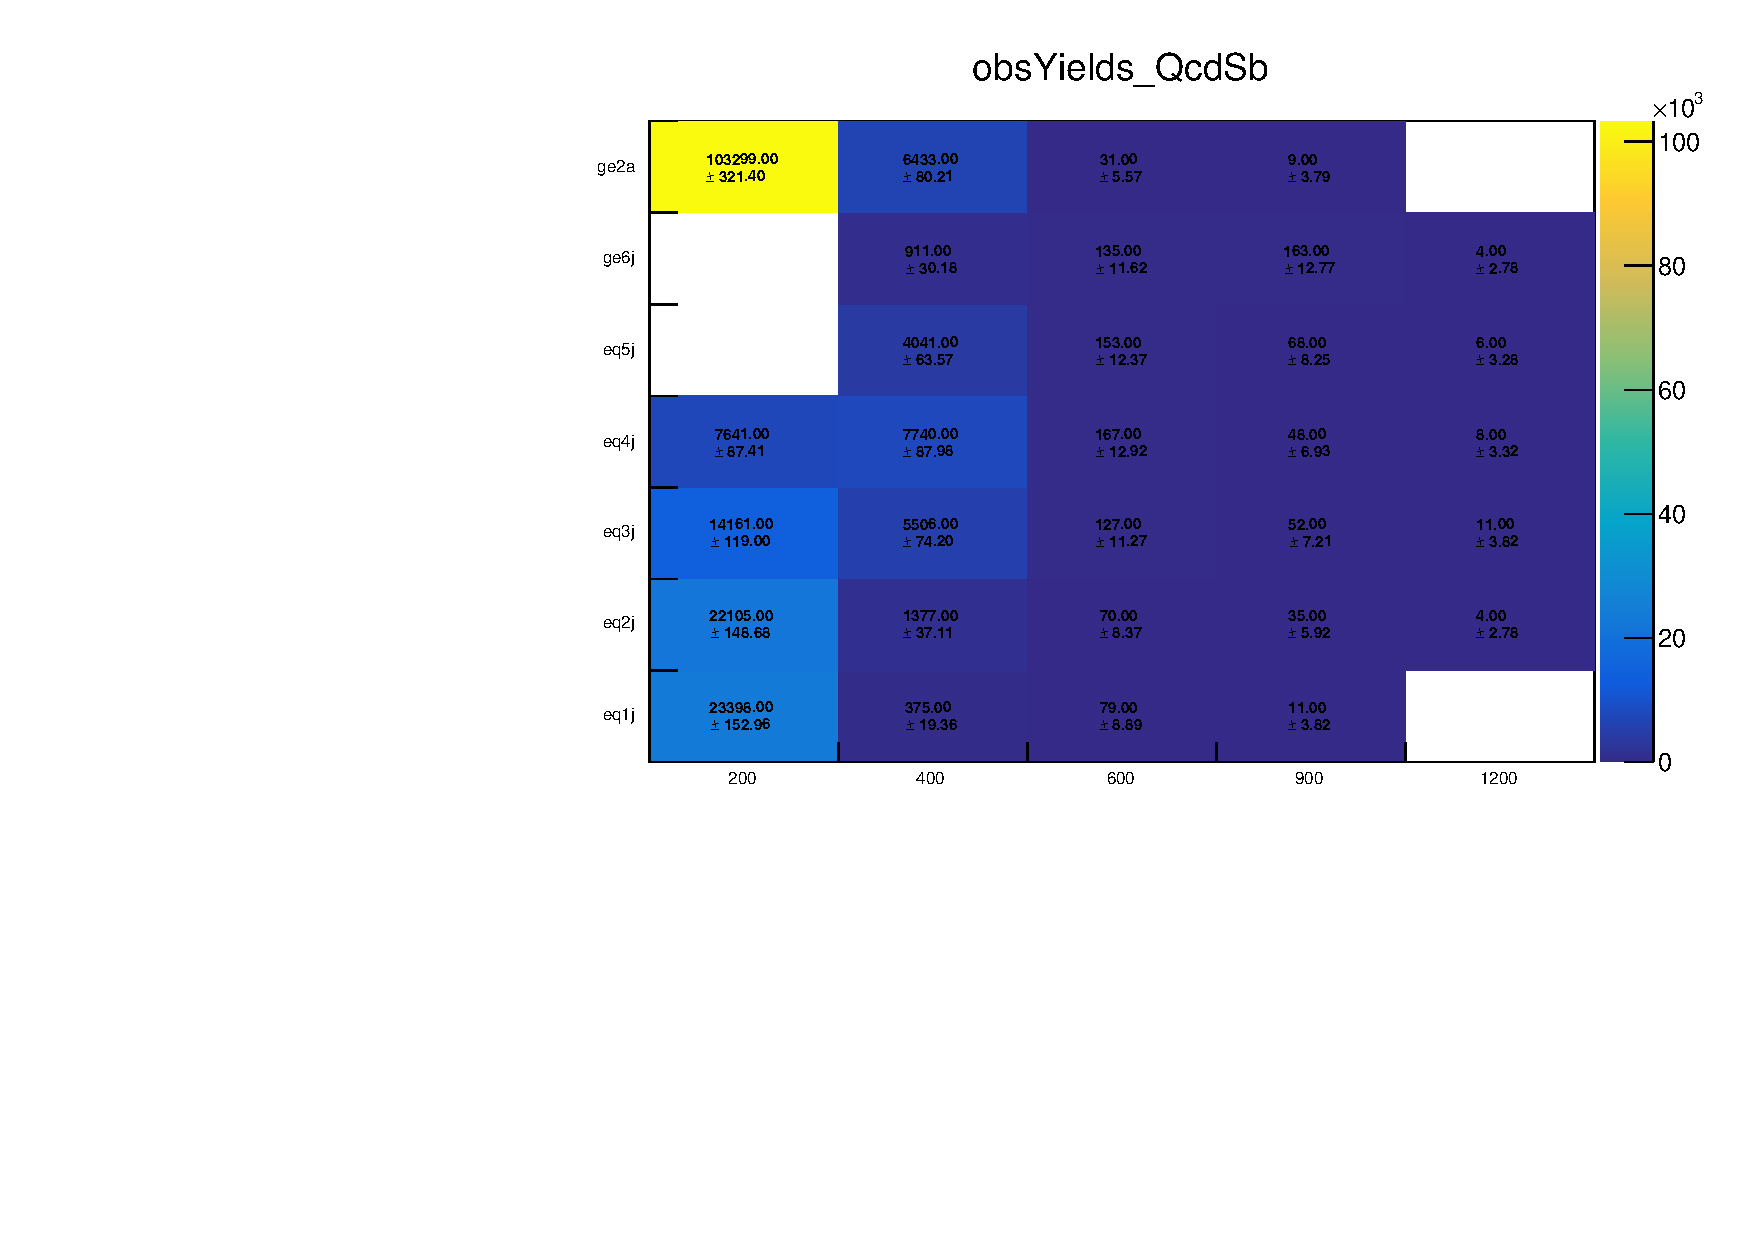
\includegraphics[width=0.5\textwidth]{figures/qcd/qcdANPlots/obsYields_QcdSb}
  } 
  \subfigure[Post-fit EWK background estimates.]{
    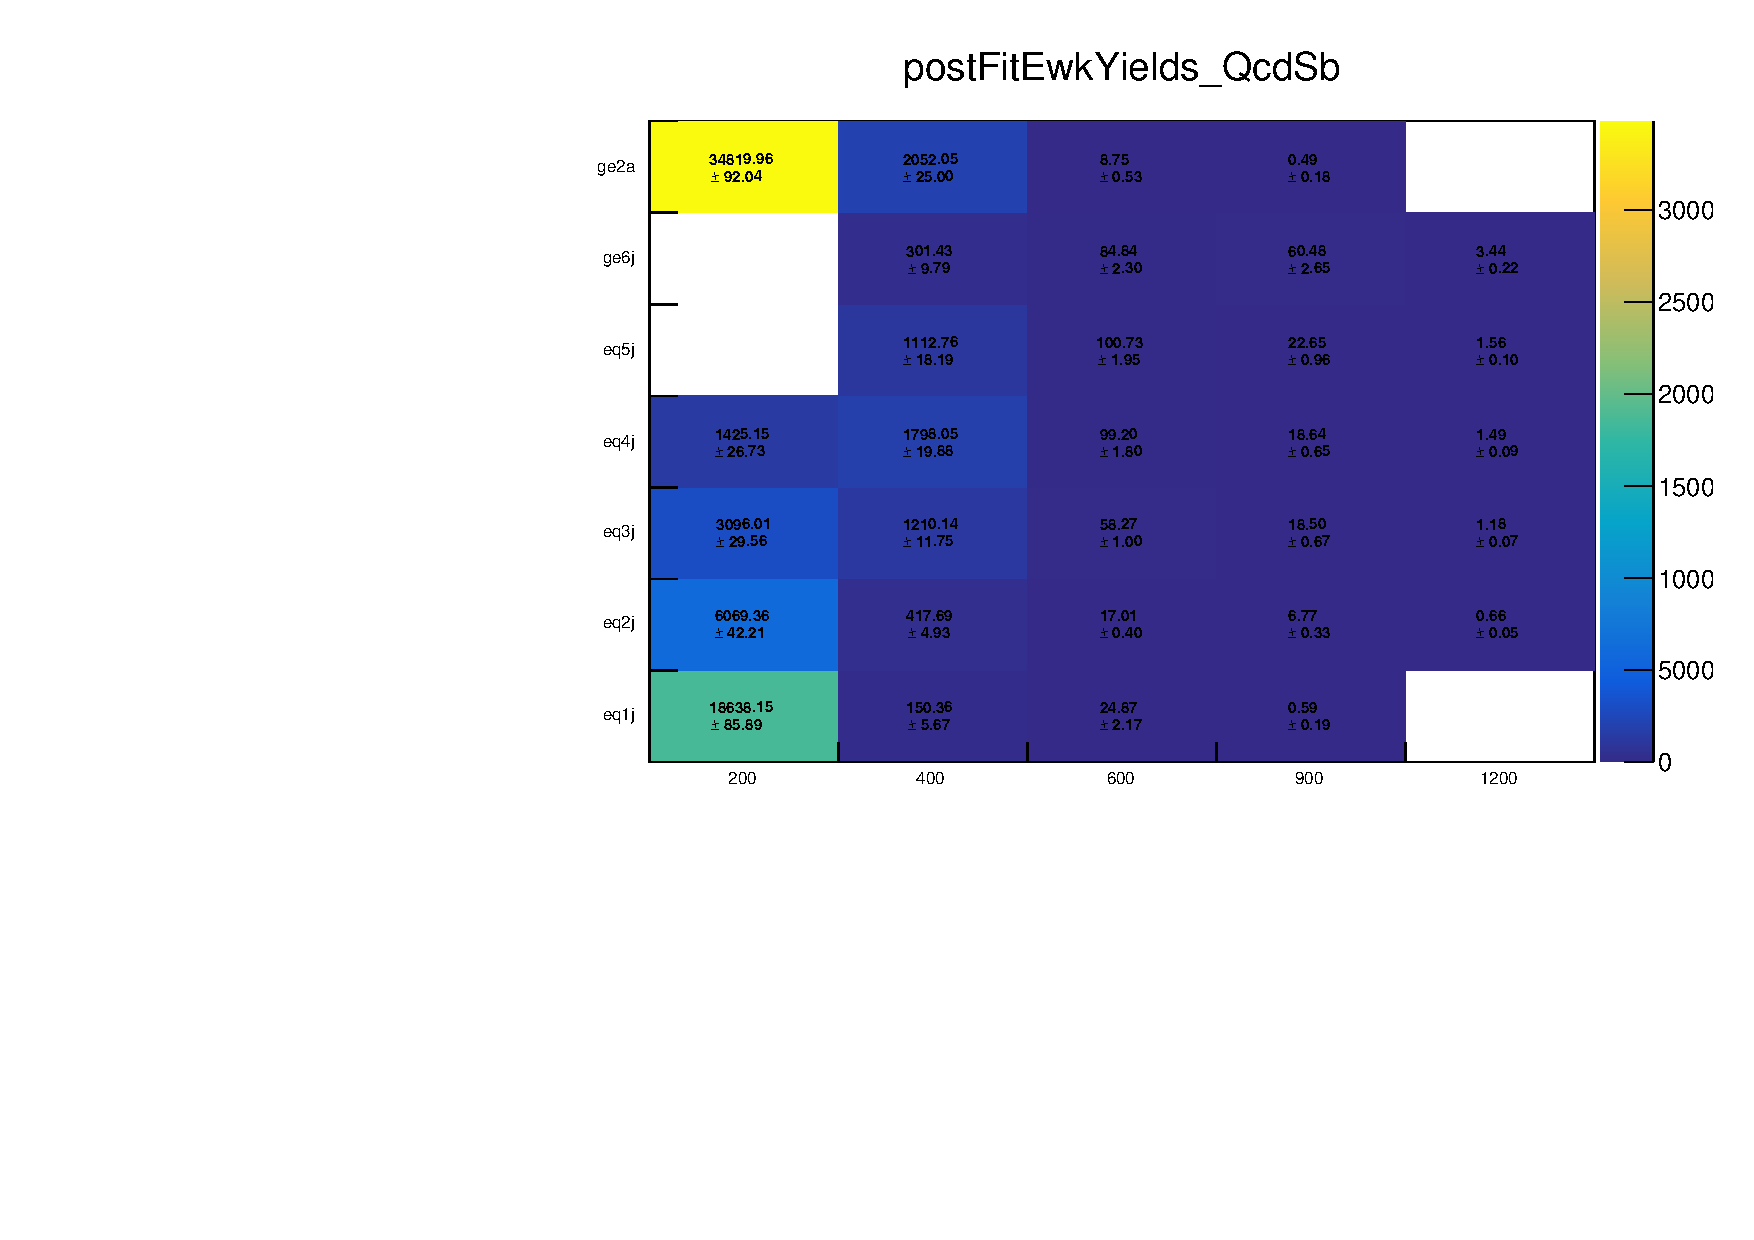
\includegraphics[width=0.5\textwidth]{figures/qcd/qcdANPlots/postFitEwkYields_QcdSb}
  } \\
  \subfigure[Post-fit constraints on $\mu_{\textrm{QCD}}$.]{
    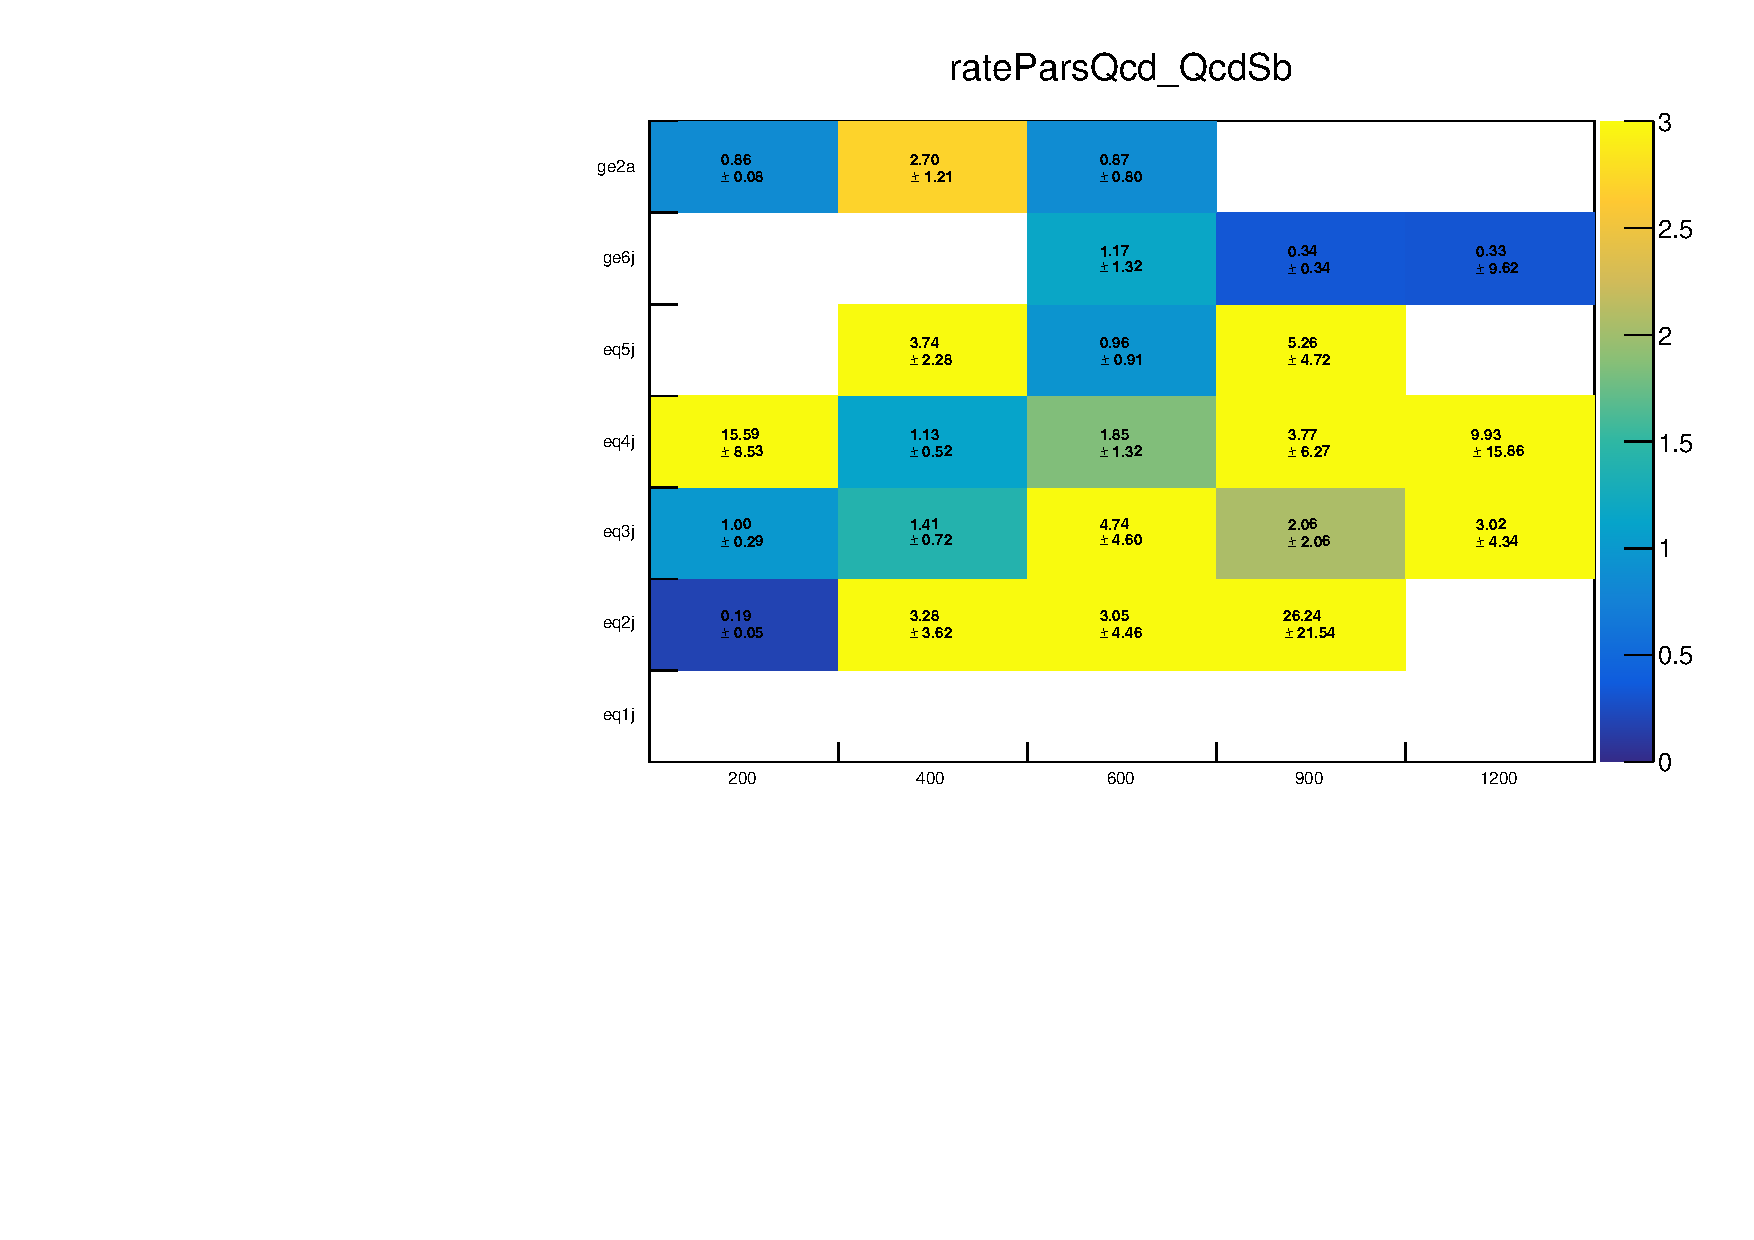
\includegraphics[width=0.5\textwidth]{figures/qcd/qcdANPlots/rateParsQcd_QcdSb}
  } 
  \subfigure[Post-fit QCD background estimates.]{
    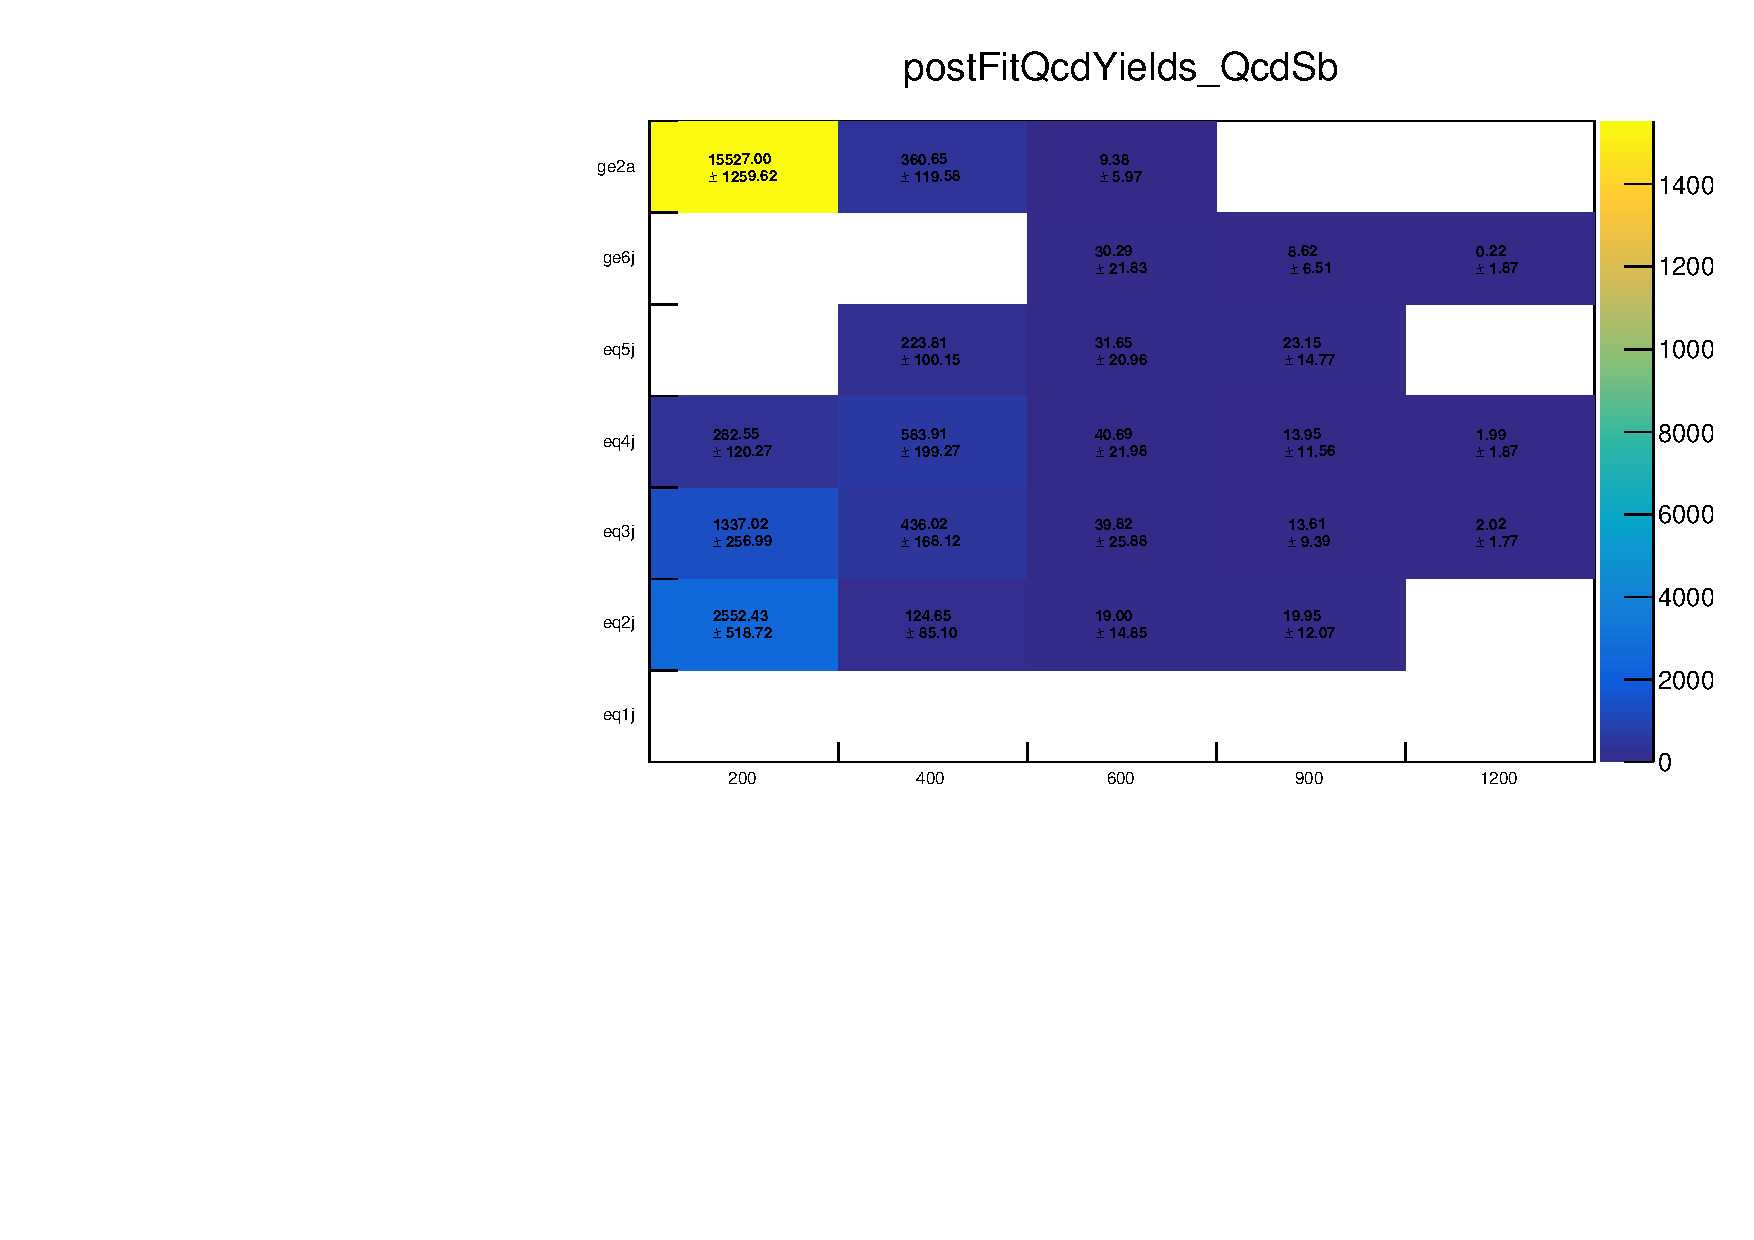
\includegraphics[width=0.5\textwidth]{figures/qcd/qcdANPlots/postFitQcdYields_QcdSb}
  } \\
  \caption{Data counts, post-fit estimates of the EWK and QCD
    background contributions, and the constrained values of the
    floating parameters $\mu_{\textrm{QCD}}$, in (\njet, \scalht) bins
    of the \mhtmet sideband (region ``B'' in Table~\ref{tab:qcd_sidebands}).}
  \label{fig:mhtmet_sideband}
\end{figure}

\clearpage
\begin{figure}[!t]
  \centering
  \subfigure[Pass/fail ratios \rmhtmet.]{
    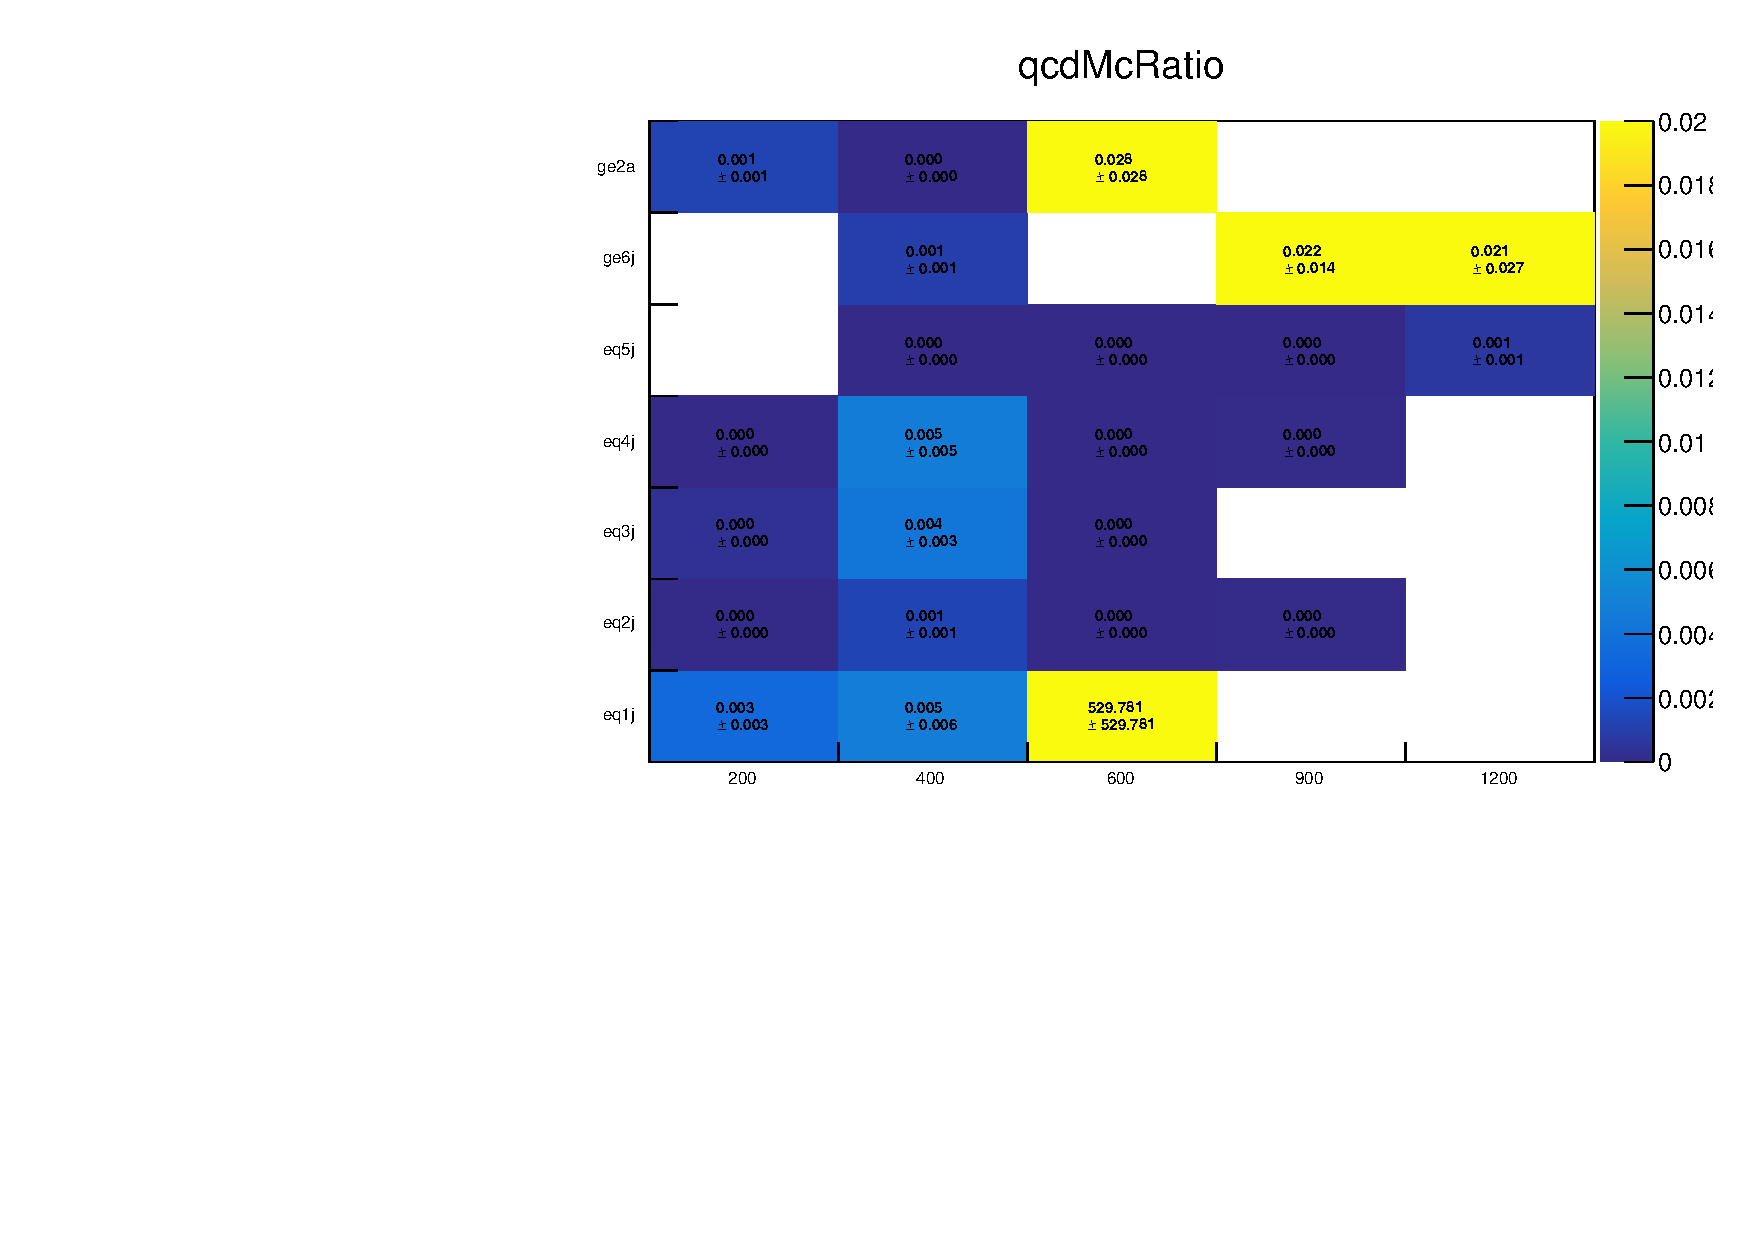
\includegraphics[width=0.5\textwidth]{figures/qcd/qcdANPlots/signalQcdDivSbQcd_MC}
  } 
  \subfigure[QCD background estimates.]{
    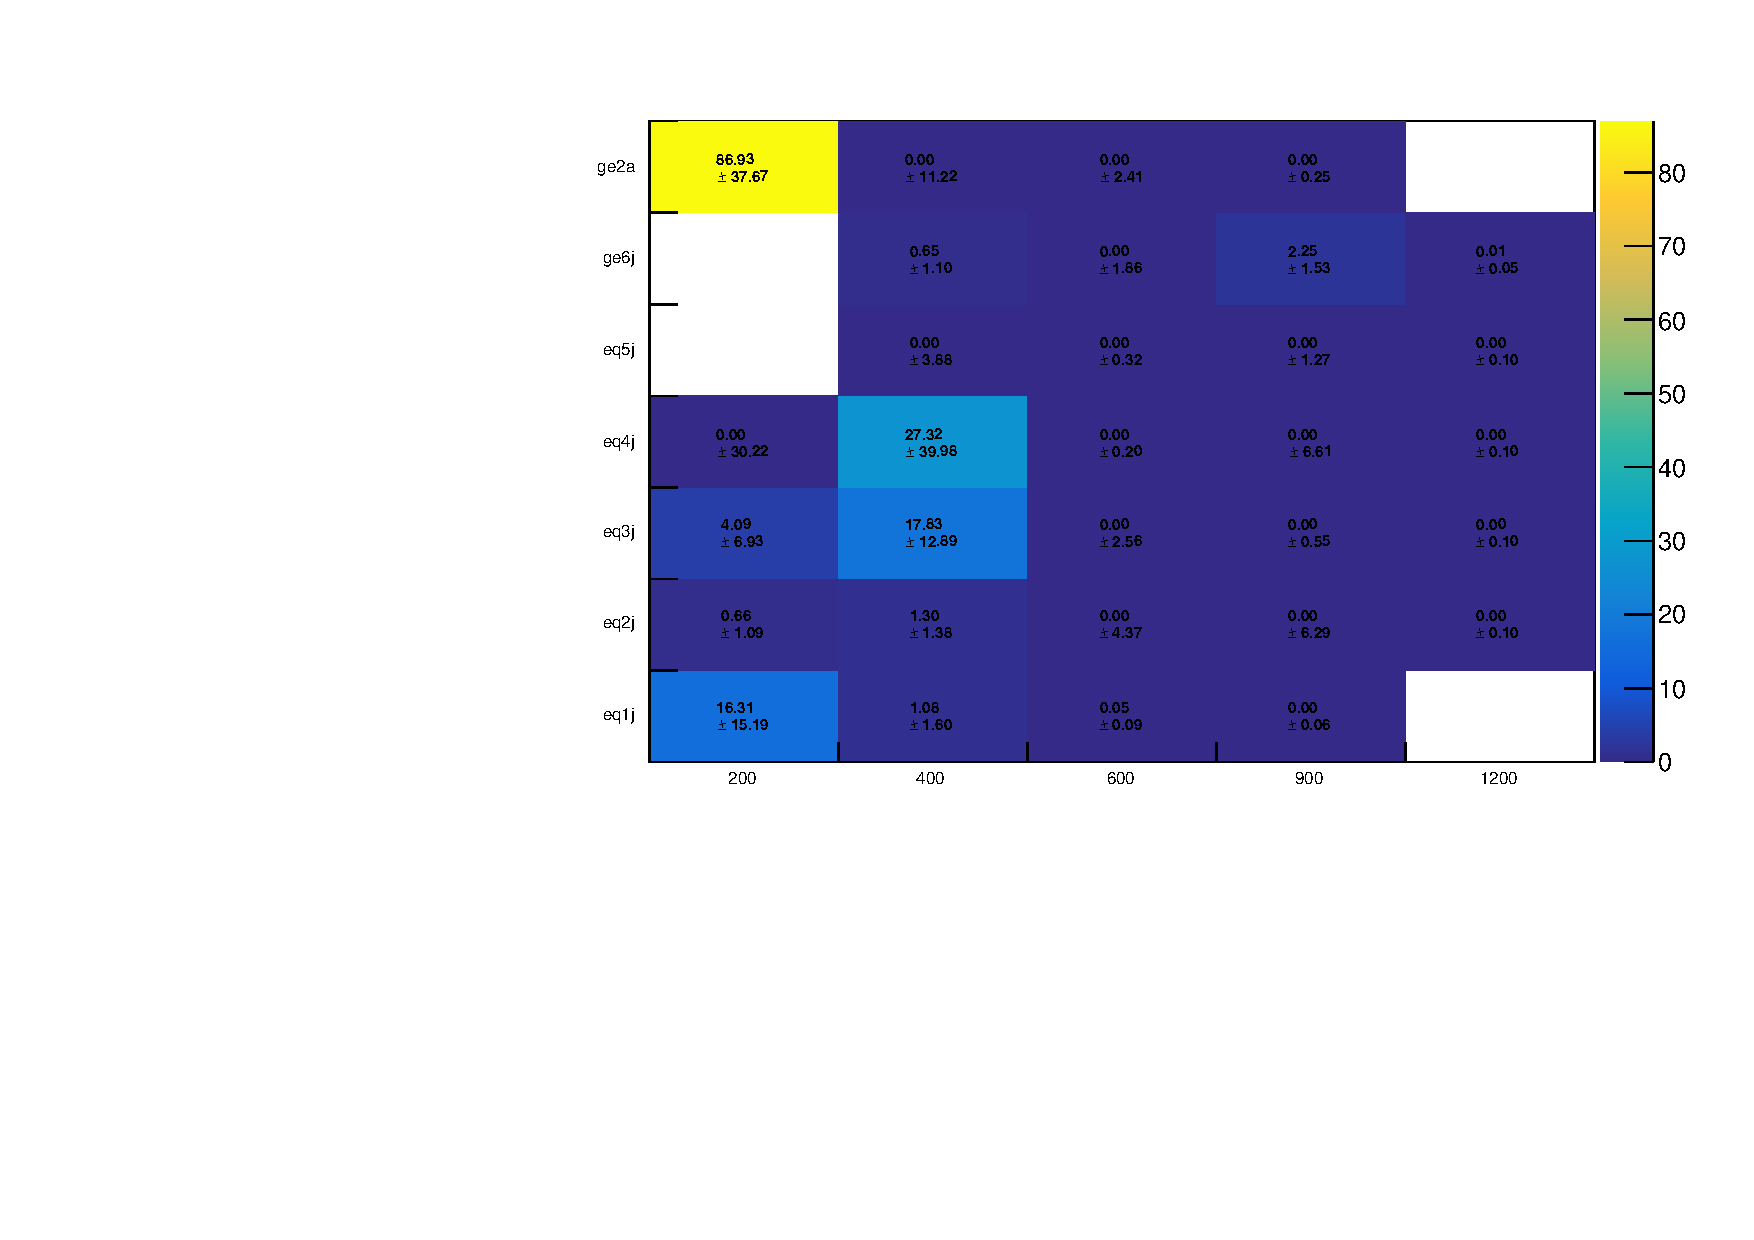
\includegraphics[width=0.5\textwidth]{figures/qcd/qcdANPlots/predictedQcdYields_Signal}
  } \\
  \subfigure[EWK background estimates.]{
    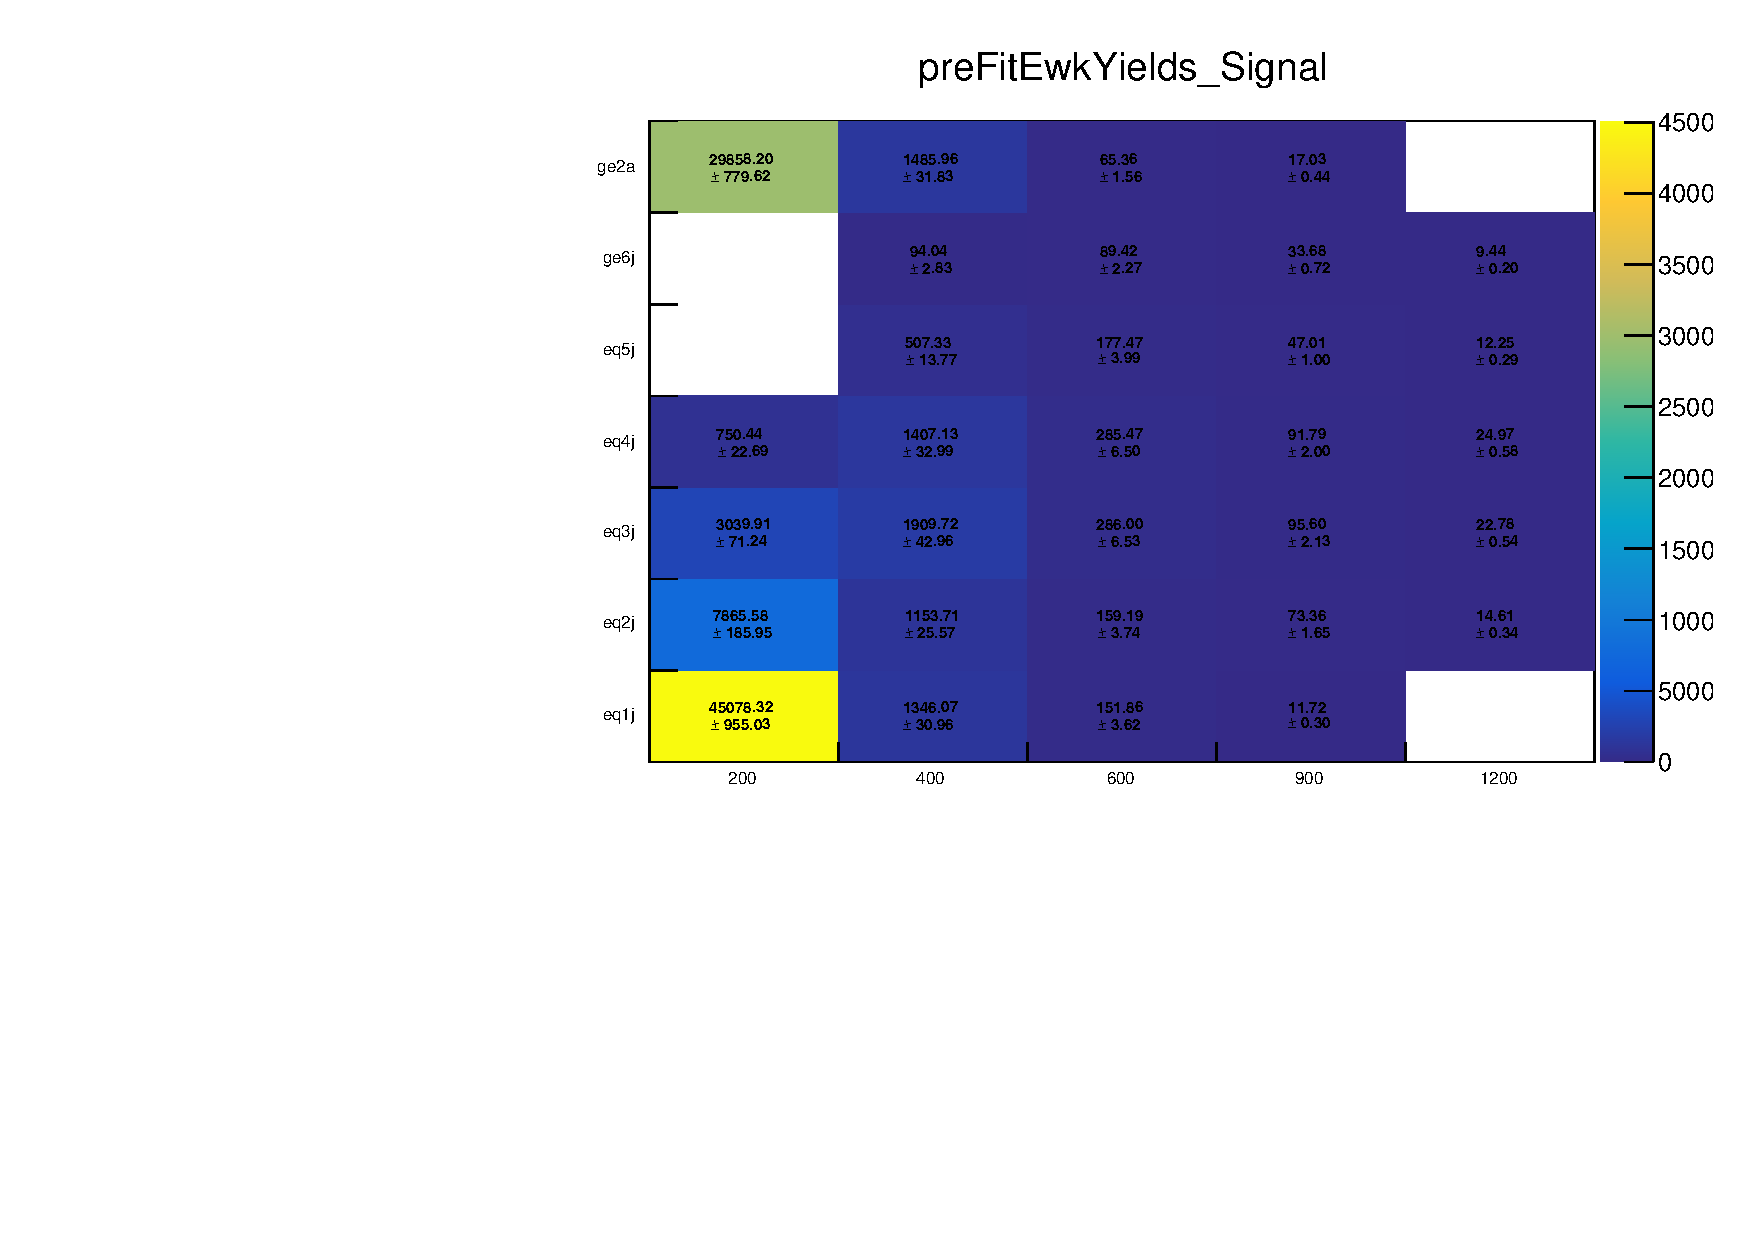
\includegraphics[width=0.5\textwidth]{figures/qcd/qcdANPlots/predictedEwkYields_Signal.pdf}
  } 
  \subfigure[Ratios of QCD/EWK background estimates.]{
    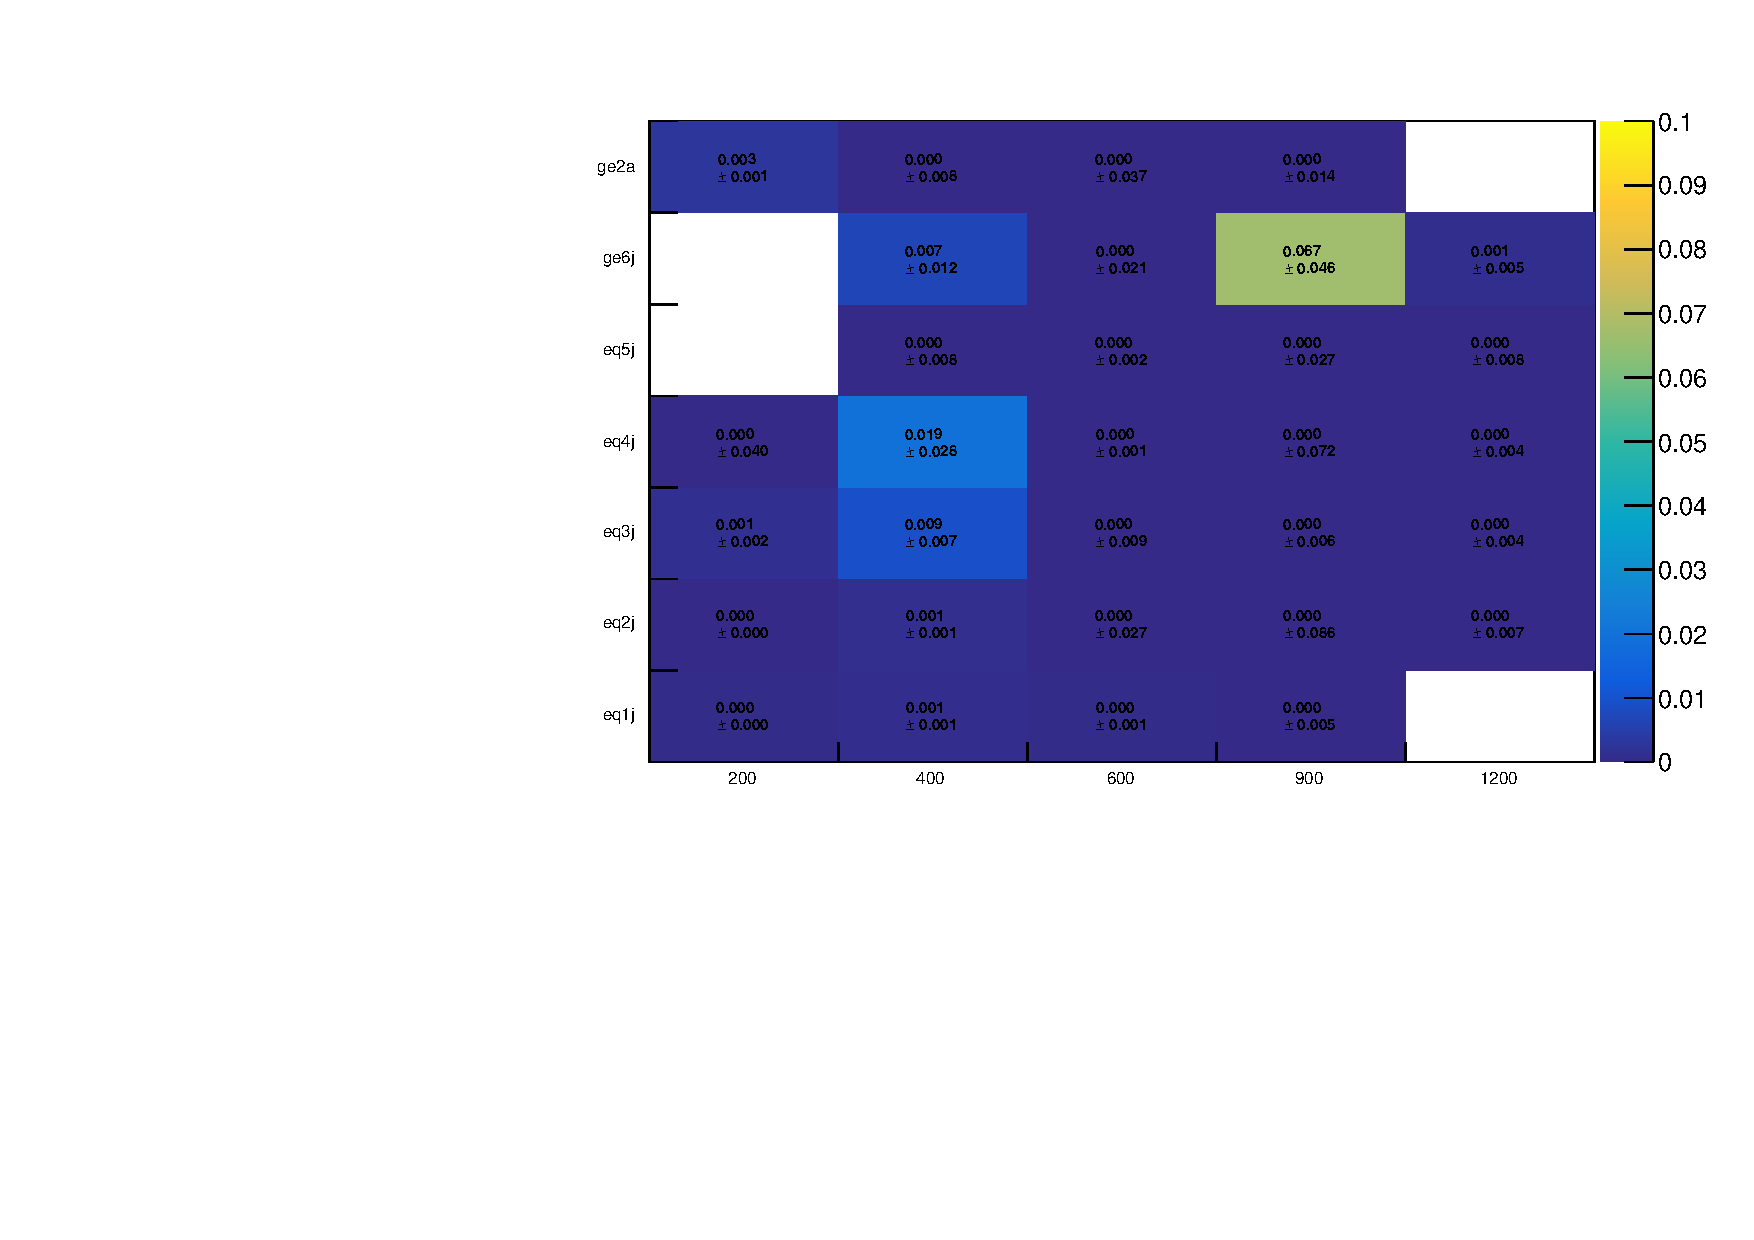
\includegraphics[width=0.5\textwidth]{figures/qcd/qcdANPlots/predictedQcdDivEwk_Signal}
  } \\
  \caption{The pass/fail ratios \rmhtmet, the EWK and QCD background
    predictions, and the ratio of QCD/EWK predictions in the signal
    region.}
  \label{fig:qcd_estimate}
\end{figure}

\clearpage
\subsection{Validation}
\label{sec:qcdValidation}

The method for predicting the QCD contamination in the signal region
described in Sec.~\ref{sec:qcdMethod} relies on the ratio, \rmhtmet,
of QCD counts that is derived with simulation. This ratio is validated
with data in a further QCD-enriched sideband, where the full signal
region selection criteria are applied, except for the inverted
requirement $0.2 < \bdphi < 0.5$.

In this sideband a data driven estimation of the QCD counts is carried
out in two further sub-regions, defined by $\mhtmet < 1.25$ and $1.25
< \mhtmet < 3.0$. These sidebands are summarised in
Table~\ref{tab:qcd_sidebands}.

\begin{table}[h!]
  \caption{Definition of sidebands used in the determination of the
    QCD background contributions in the signal region. }
  \label{tab:qcd_sidebands}
  \centering
  \footnotesize
  \begin{tabular}{ l|l|l }
                           & $0.2 < \bdphi < 0.5$           & $\bdphi > 0.5$                  \\[0.2ex]
    \hline
    $1.25 < \mhtmet < 3.0$ & \textbf{A} ``Double sideband'' & \textbf{B} ``\mhtmet sideband'' \\[0.2ex]
    \hline
    $\mhtmet < 1.25$       & \textbf{C} ``\bdphi sideband'' & \textbf{D} ``Signal region''    \\[0.2ex]
  \end{tabular}
\end{table}

To validate the ratio \rmhtmet it is assumed that if the simulation of
the ratio in the \bdphi sideband agrees with that derived from data,
the simulated ratio that is not in the sideband is valid. Any
disagreement is covered by a systematic error on the signal region QCD
prediction. The double ratio of $\rmhtmet_{\bdphi<0.5}$ and
$\rmhtmet_{\bdphi<0.5}^{data}$ in \scalht and \njet bins is shown in
Fig.~\ref{fig:RR_qcd}. Bins in which there are insufficient statistics
in data or simulation to make the calculation are left out.  This plot
illustrates that a fully correlated systematic of 100\% taken on the
predicted QCD contamination in the signal region should cover any
disagreement between simulation and data.

As the prediction of QCD in the signal region is carried out
inclusively over \nb and \mht, the QCD shapes for these variables are
taken from the EWK simulation and normalised to the QCD counts. 
A lack of statistics in
the QCD MC led to the adoption of this approach. 
% To validate it, the simulated \mht distributions
% for the QCD and EWK processes in the signal region are divided. This is shown in
% Figs.~\ref{fig:qcd_validation}.%~\ref{fig:asym_qcd_validation}-\ref{fig:asym_qcd_validation}.
% As the normalisation is carried out independently, a flat distribution
% of the ratio is enough for validation. Within uncertainties, the level of agreement is acceptable given the
% small total QCD contribution to the signal region and its large
% systematic uncertainty.
%
\begin{figure}[h!]
  \begin{center}        
    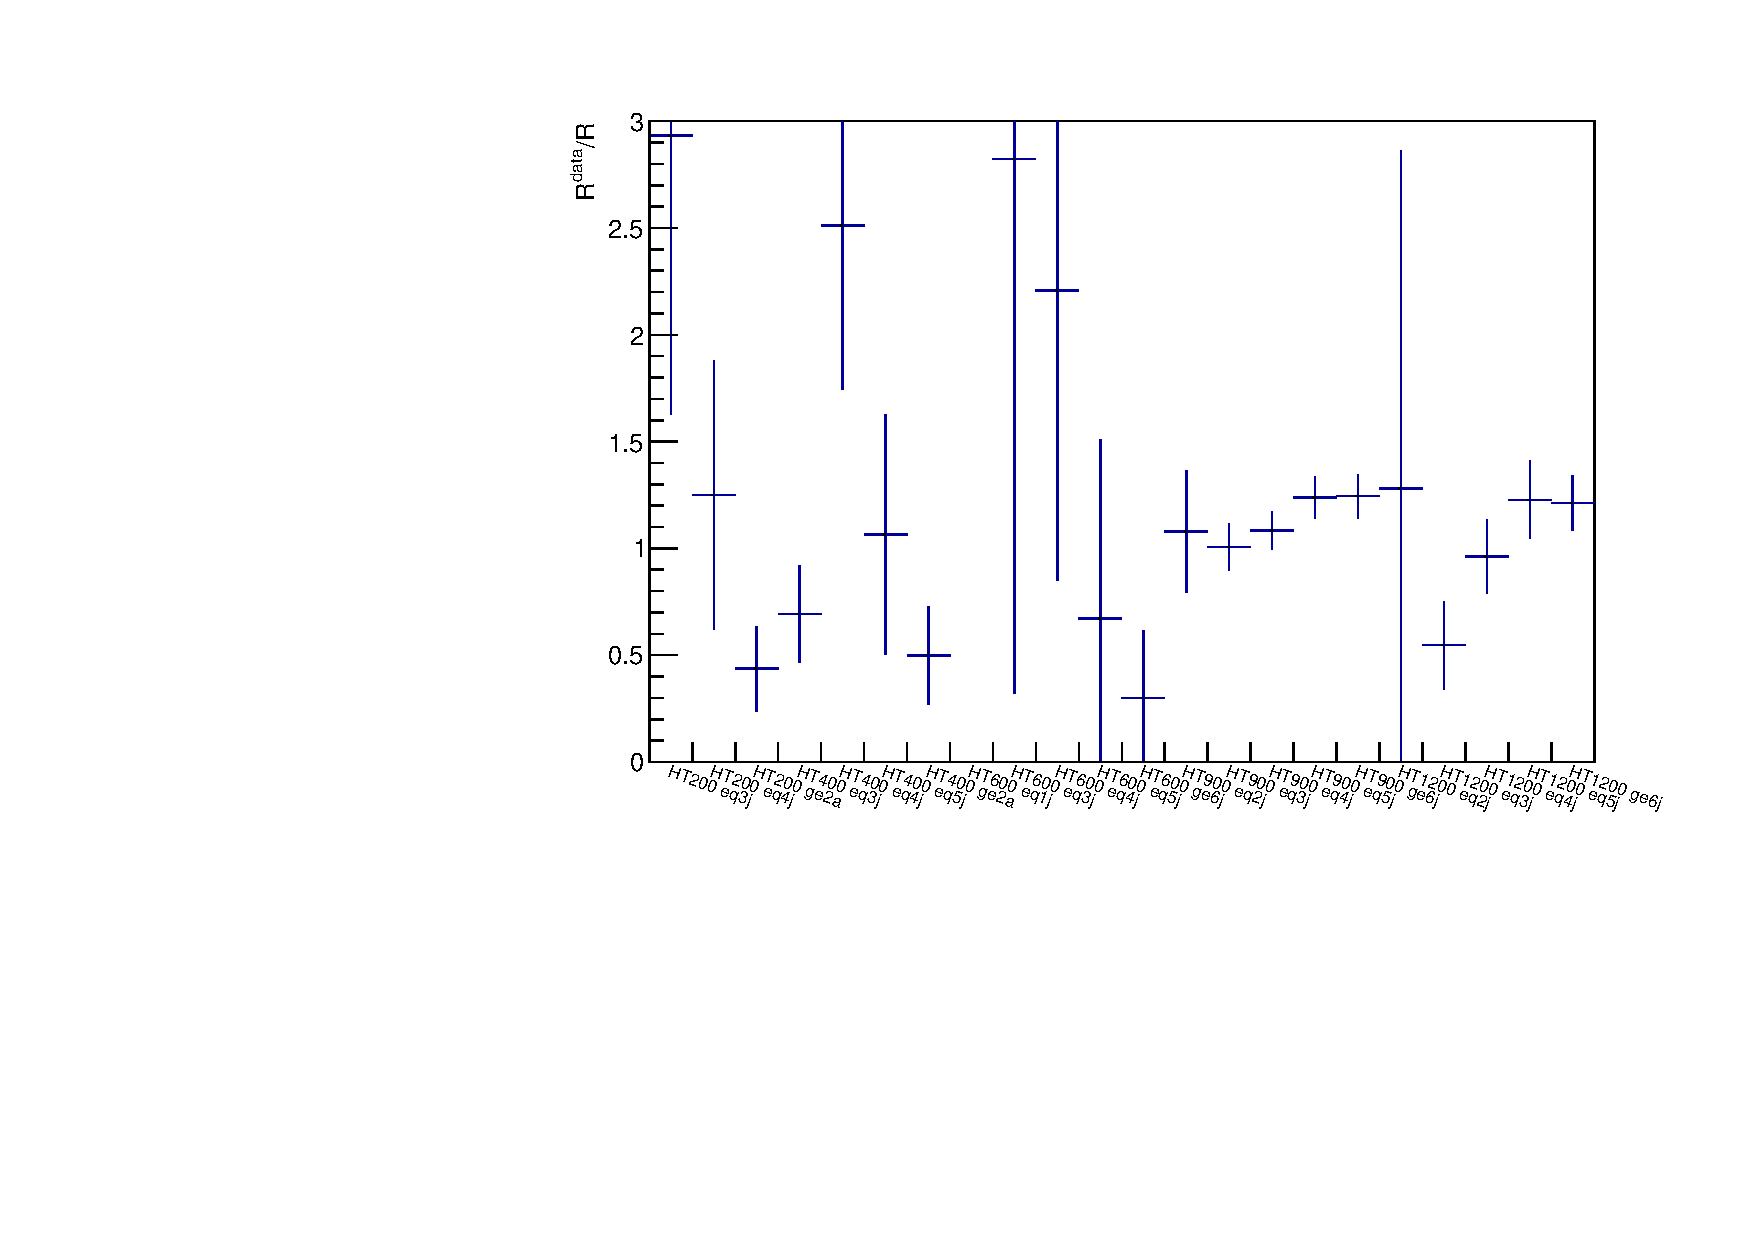
\includegraphics[width=\textwidth]{figures/qcd/qcdANPlots/doubleQcdSbSrRatio1D}
    \caption{ Ratio of the measurement of \rmhtmet, the pass/fail
      ratio for the \mhtmet selection, from data and Monte Carlo in
      the $\bdphi < 0.5$ sideband in (\scalht, \njet) bins.   
    }
    \label{fig:RR_qcd}
  \end{center} 
\end{figure}

\clearpage
\begin{figure}[!t]
  \centering
  \subfigure[Data counts.]{
    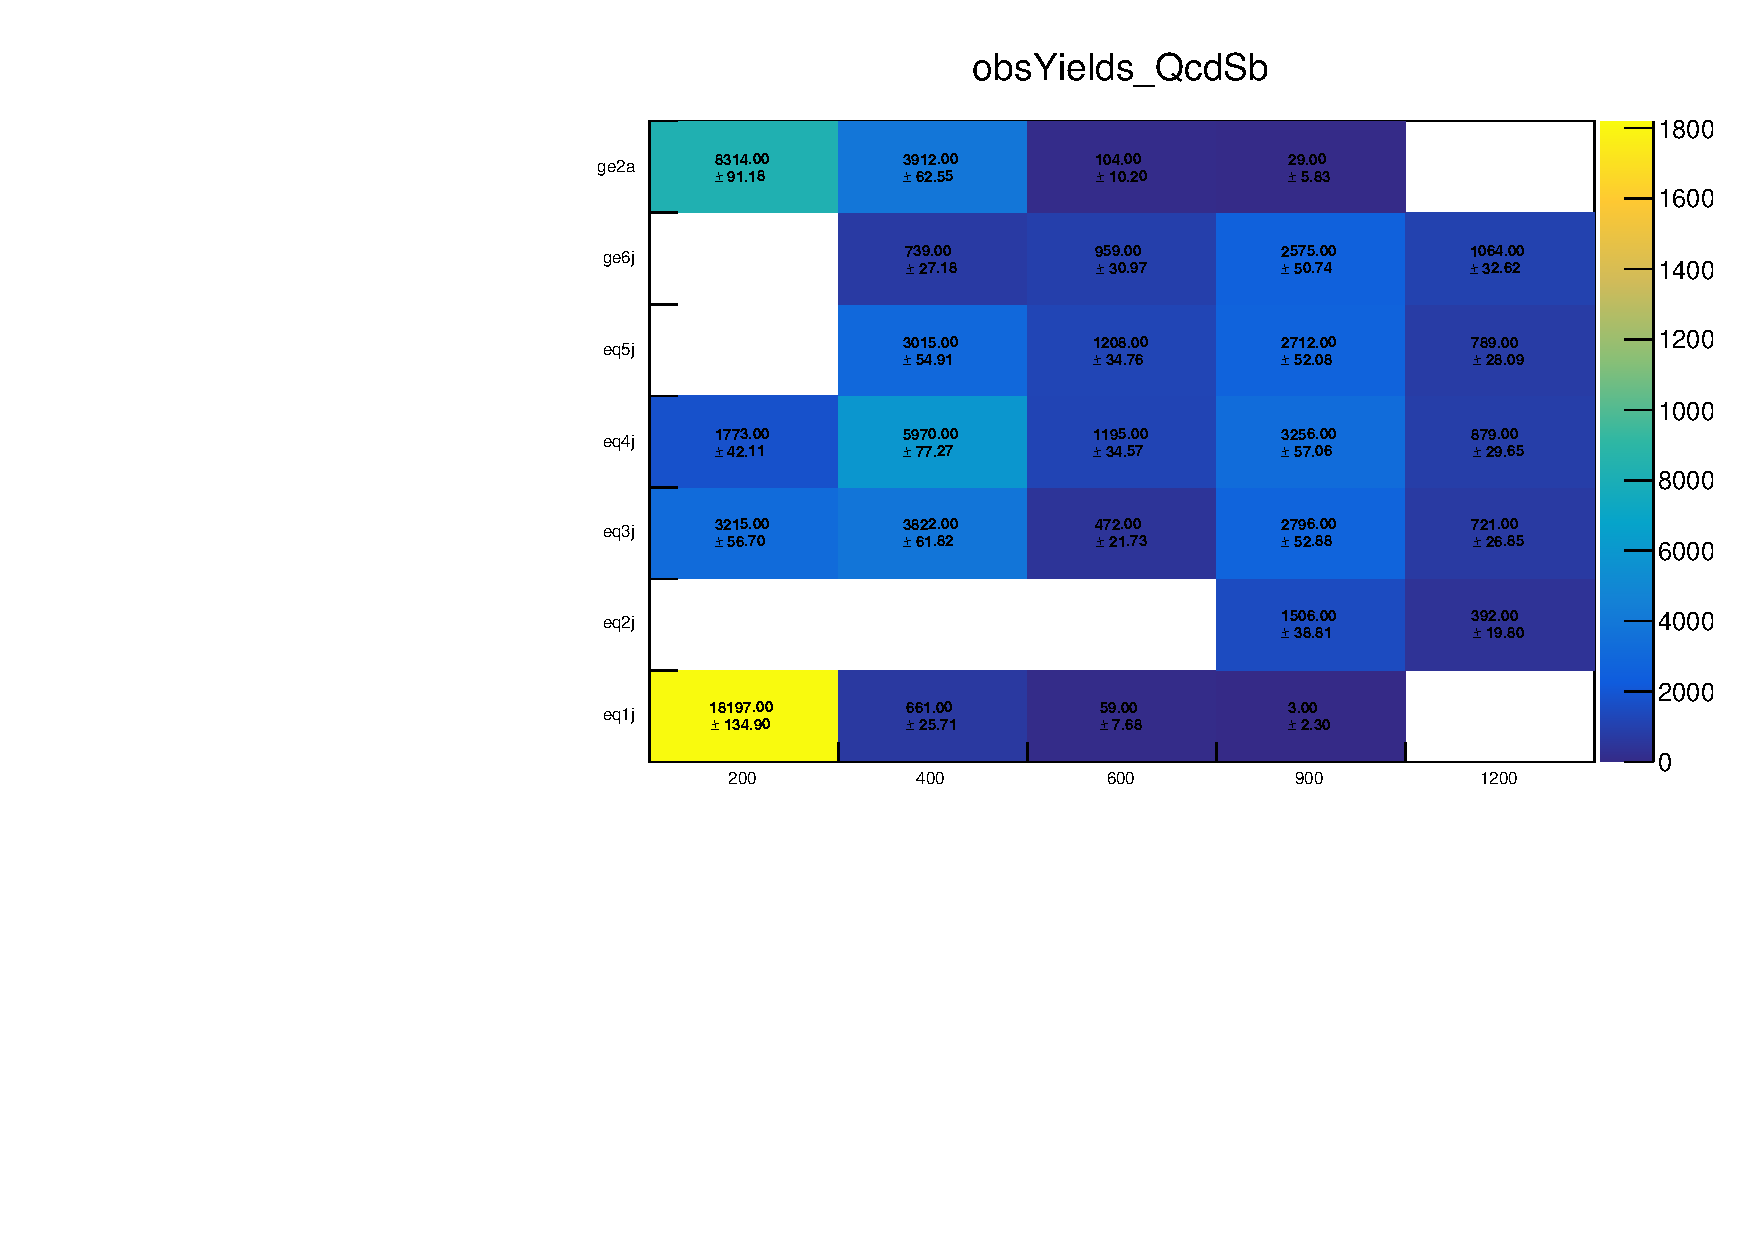
\includegraphics[width=0.5\textwidth]{figures/qcd/qcdANPlotsBDPhiSb/obsYields_QcdSb}
  } 
  \subfigure[Post-fit EWK background estimates.]{
    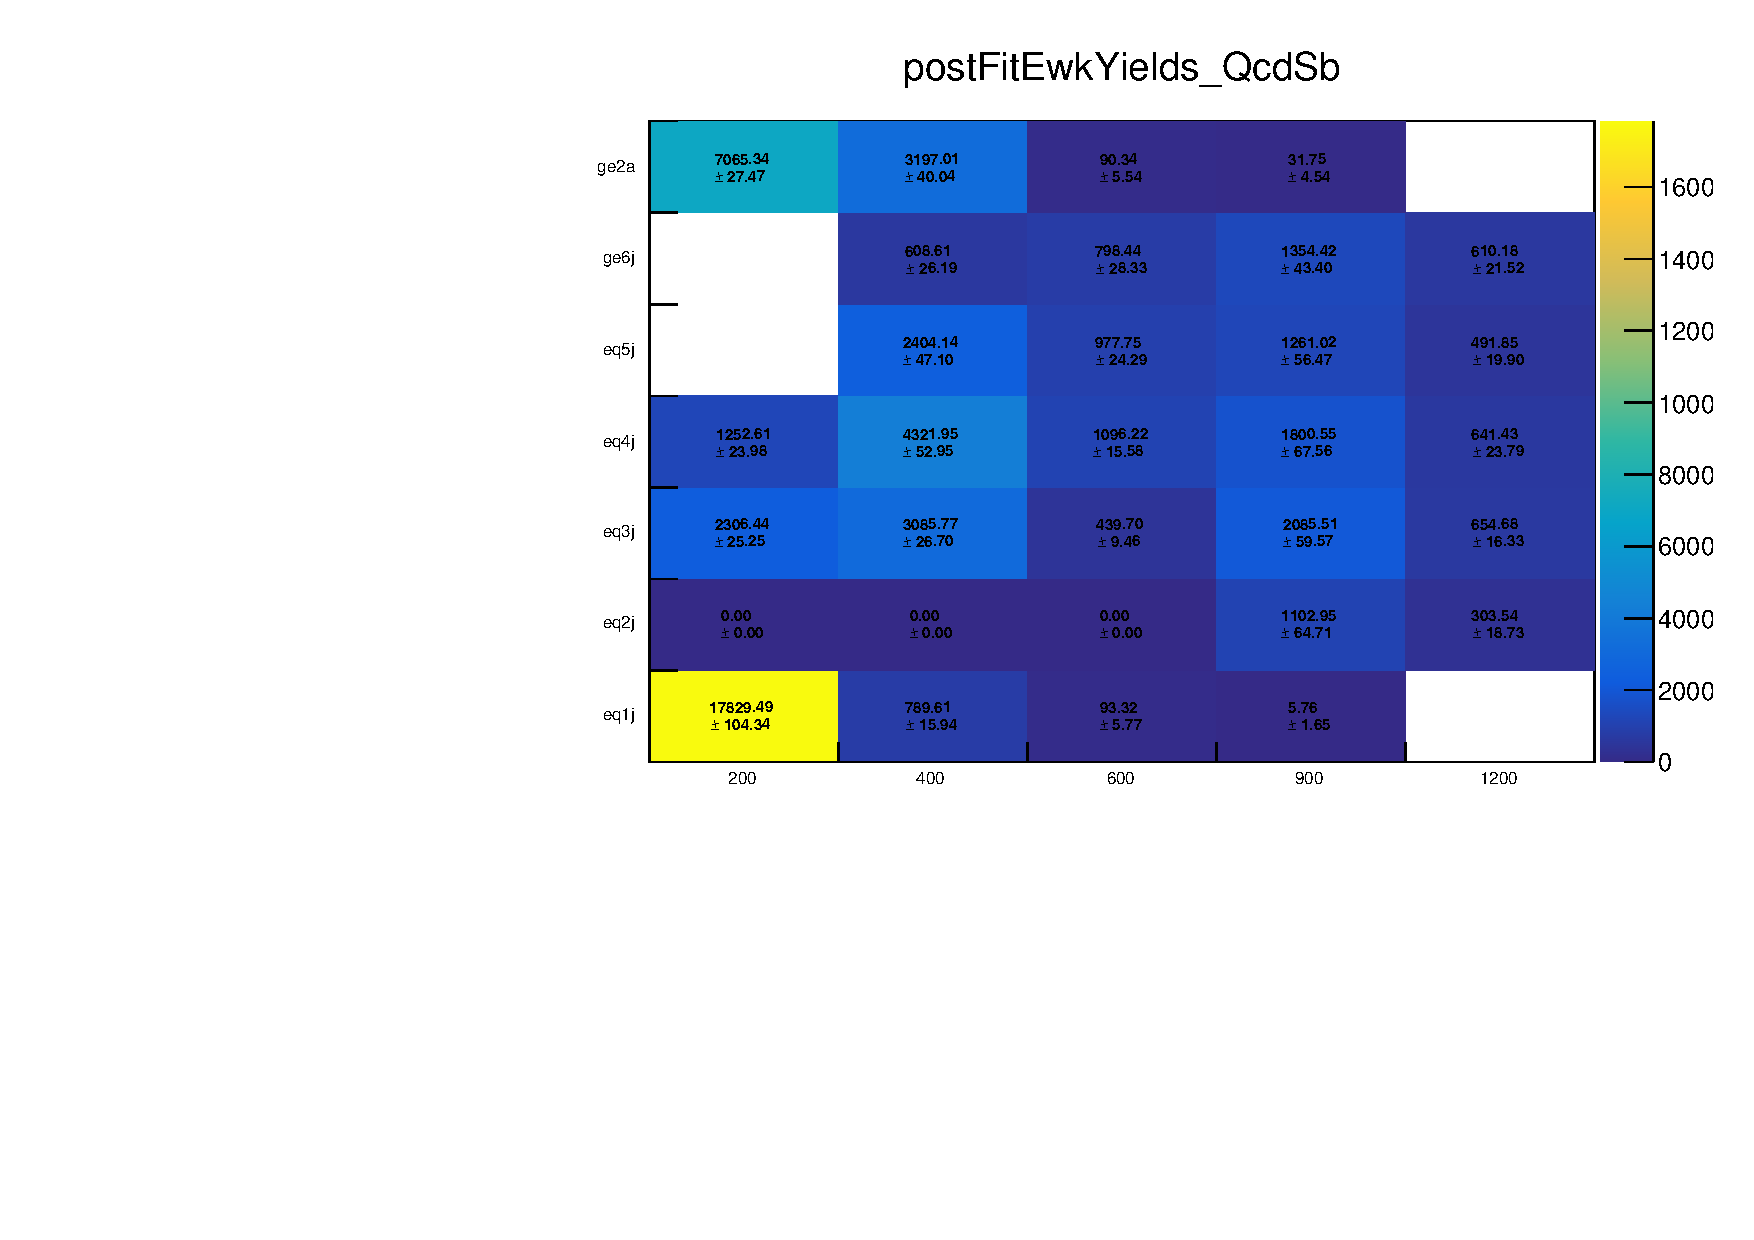
\includegraphics[width=0.5\textwidth]{figures/qcd/qcdANPlotsBDPhiSb/postFitEwkYields_QcdSb}
  } \\
  \subfigure[Post-fit constraints on $\mu_{\textrm{QCD}}$.]{
    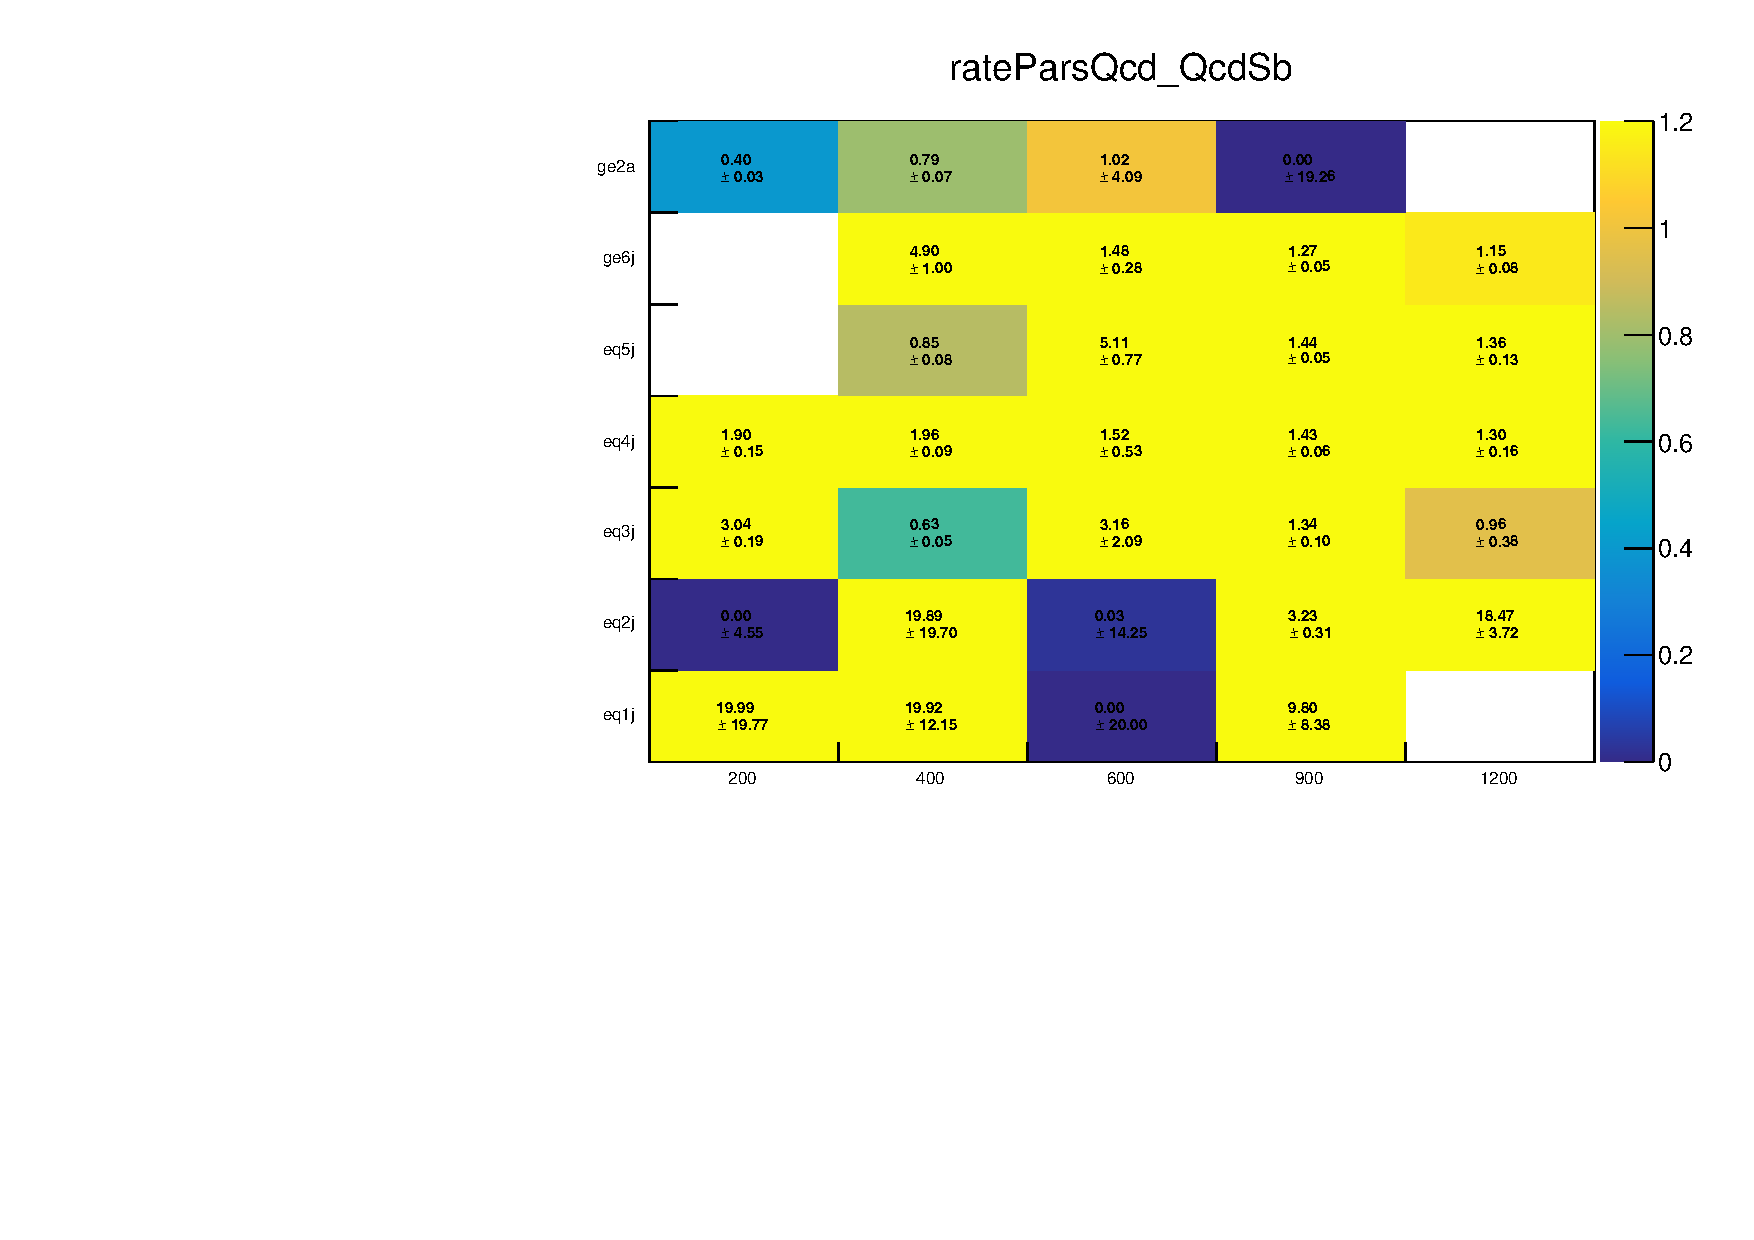
\includegraphics[width=0.5\textwidth]{figures/qcd/qcdANPlotsBDPhiSb/rateParsQcd_QcdSb}
  } 
  \subfigure[Post-fit QCD background estimates.]{
    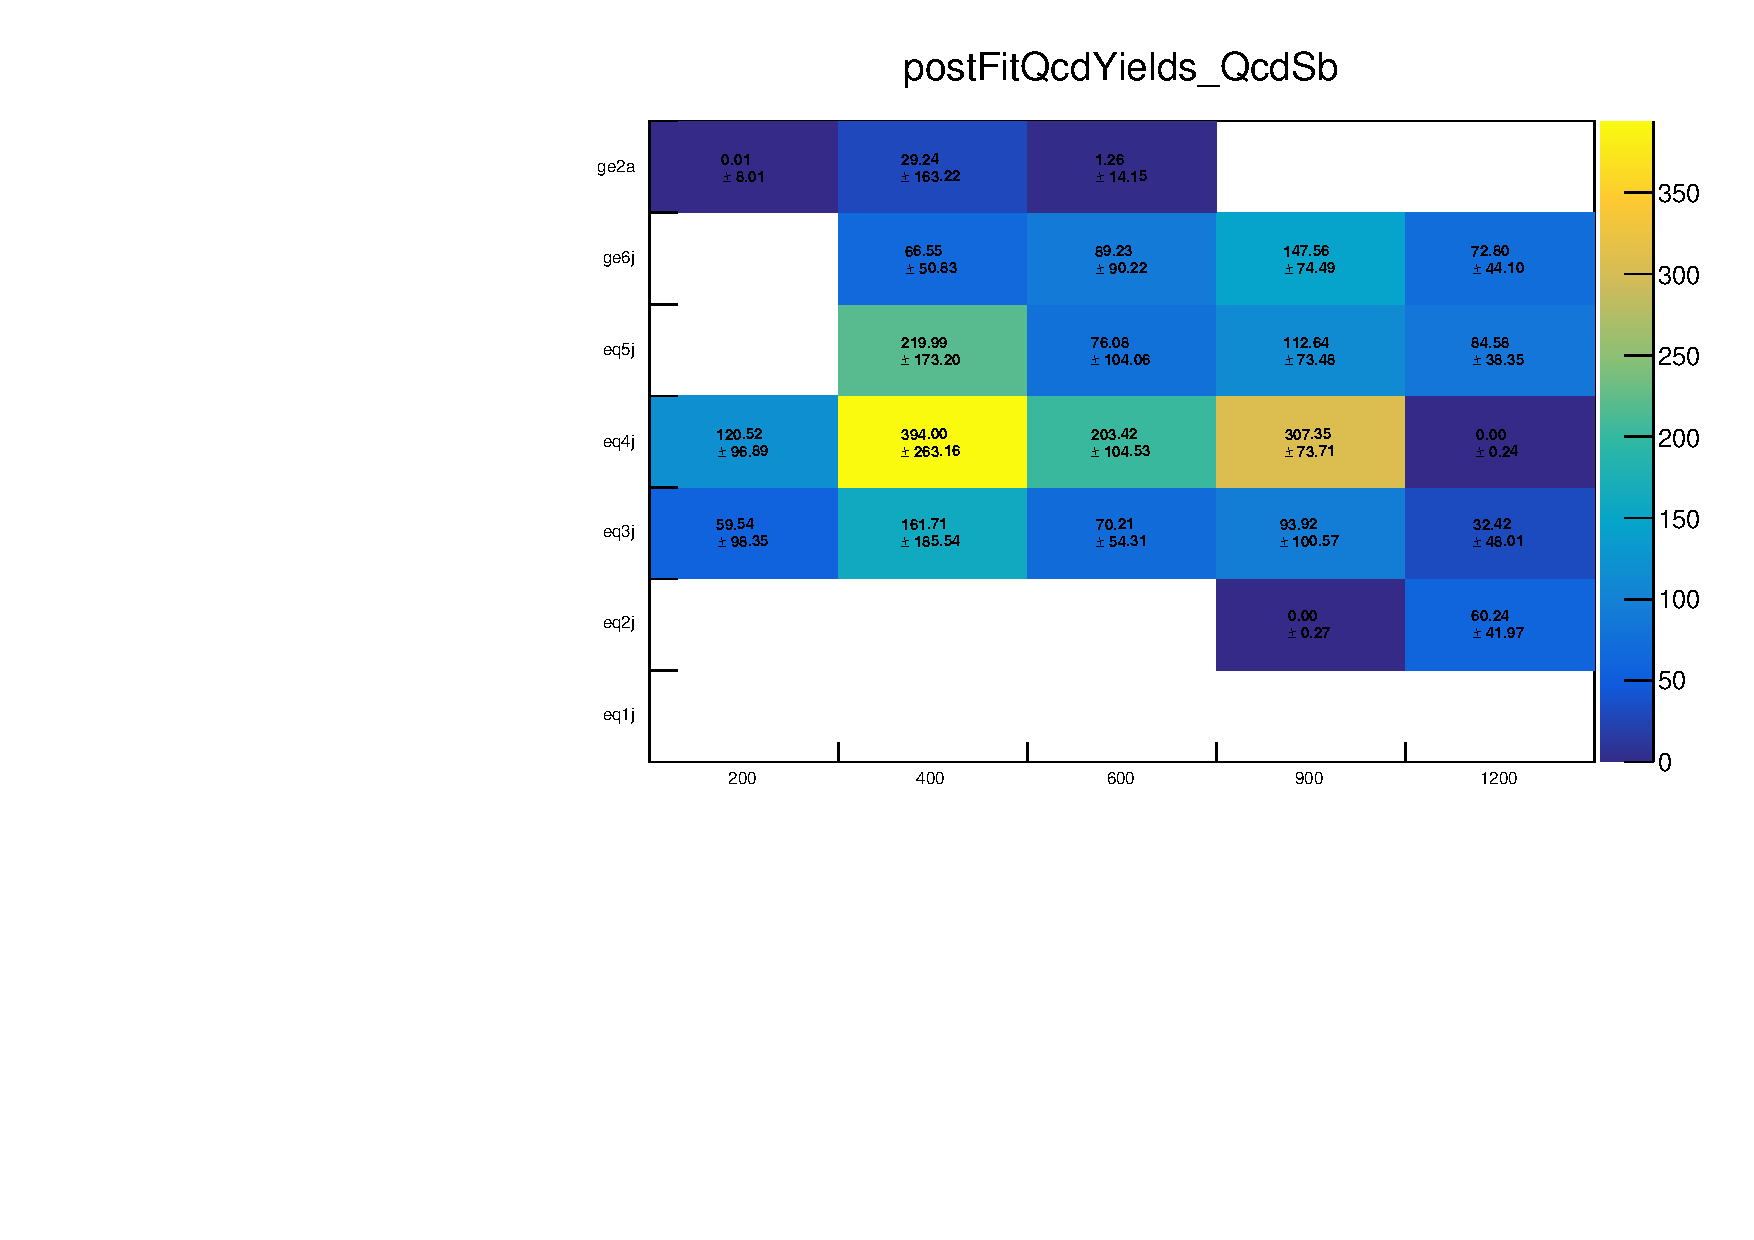
\includegraphics[width=0.5\textwidth]{figures/qcd/qcdANPlotsBDPhiSb/postFitQcdYields_QcdSb}
  } \\
  \caption{Data counts, post-fit estimates of the EWK and QCD
    background contributions, and the constrained values of the
    floating parameters $\mu_{\textrm{QCD}}$, in (\njet, \scalht) bins
    of the \bdphi sideband (region ``C'' in Table~\ref{tab:qcd_sidebands}).}
  \label{fig:mhtmet_sideband}
\end{figure}

\clearpage
\begin{figure}[!t]
  \centering
  \subfigure[Data counts.]{
    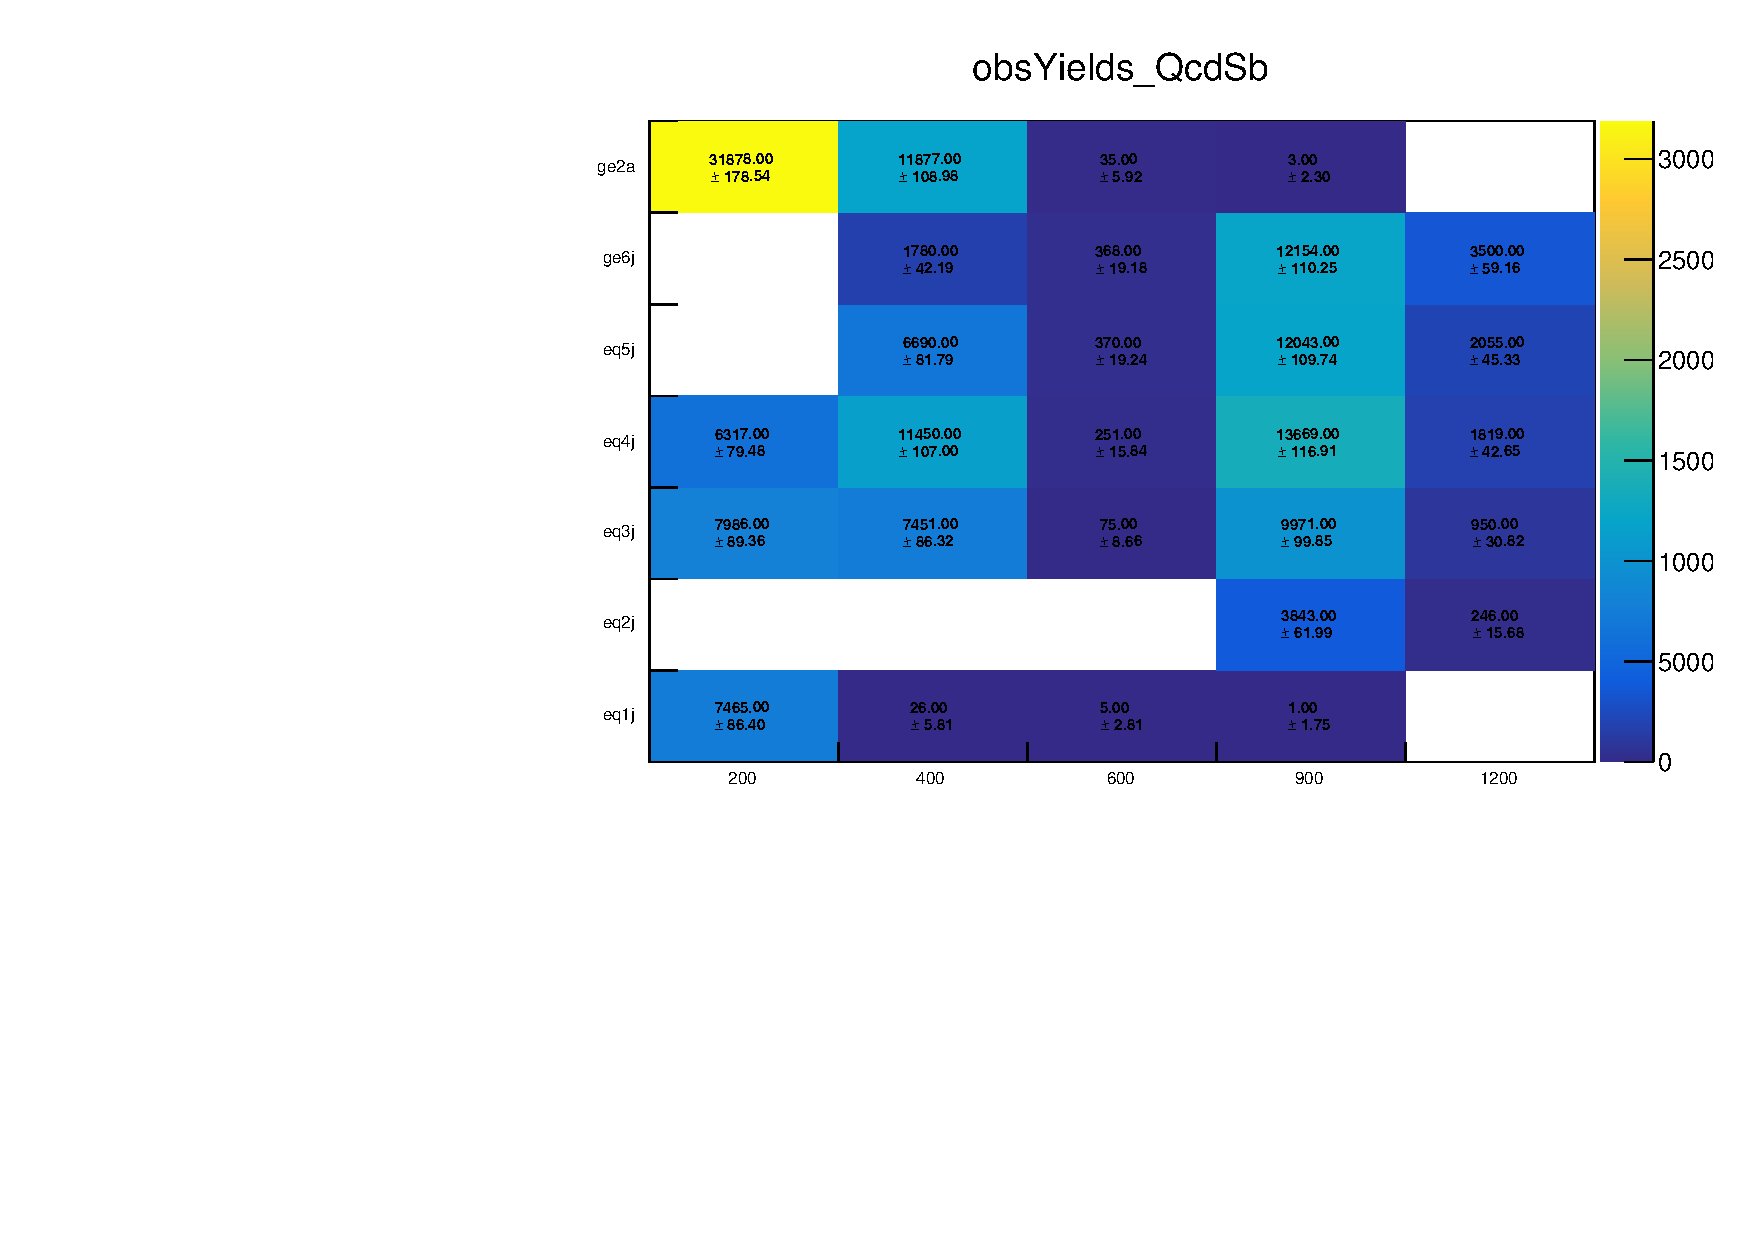
\includegraphics[width=0.5\textwidth]{figures/qcd/qcdANPlotsDoubleSb/obsYields_QcdSb}
  } 
  \subfigure[Post-fit EWK background estimates.]{
    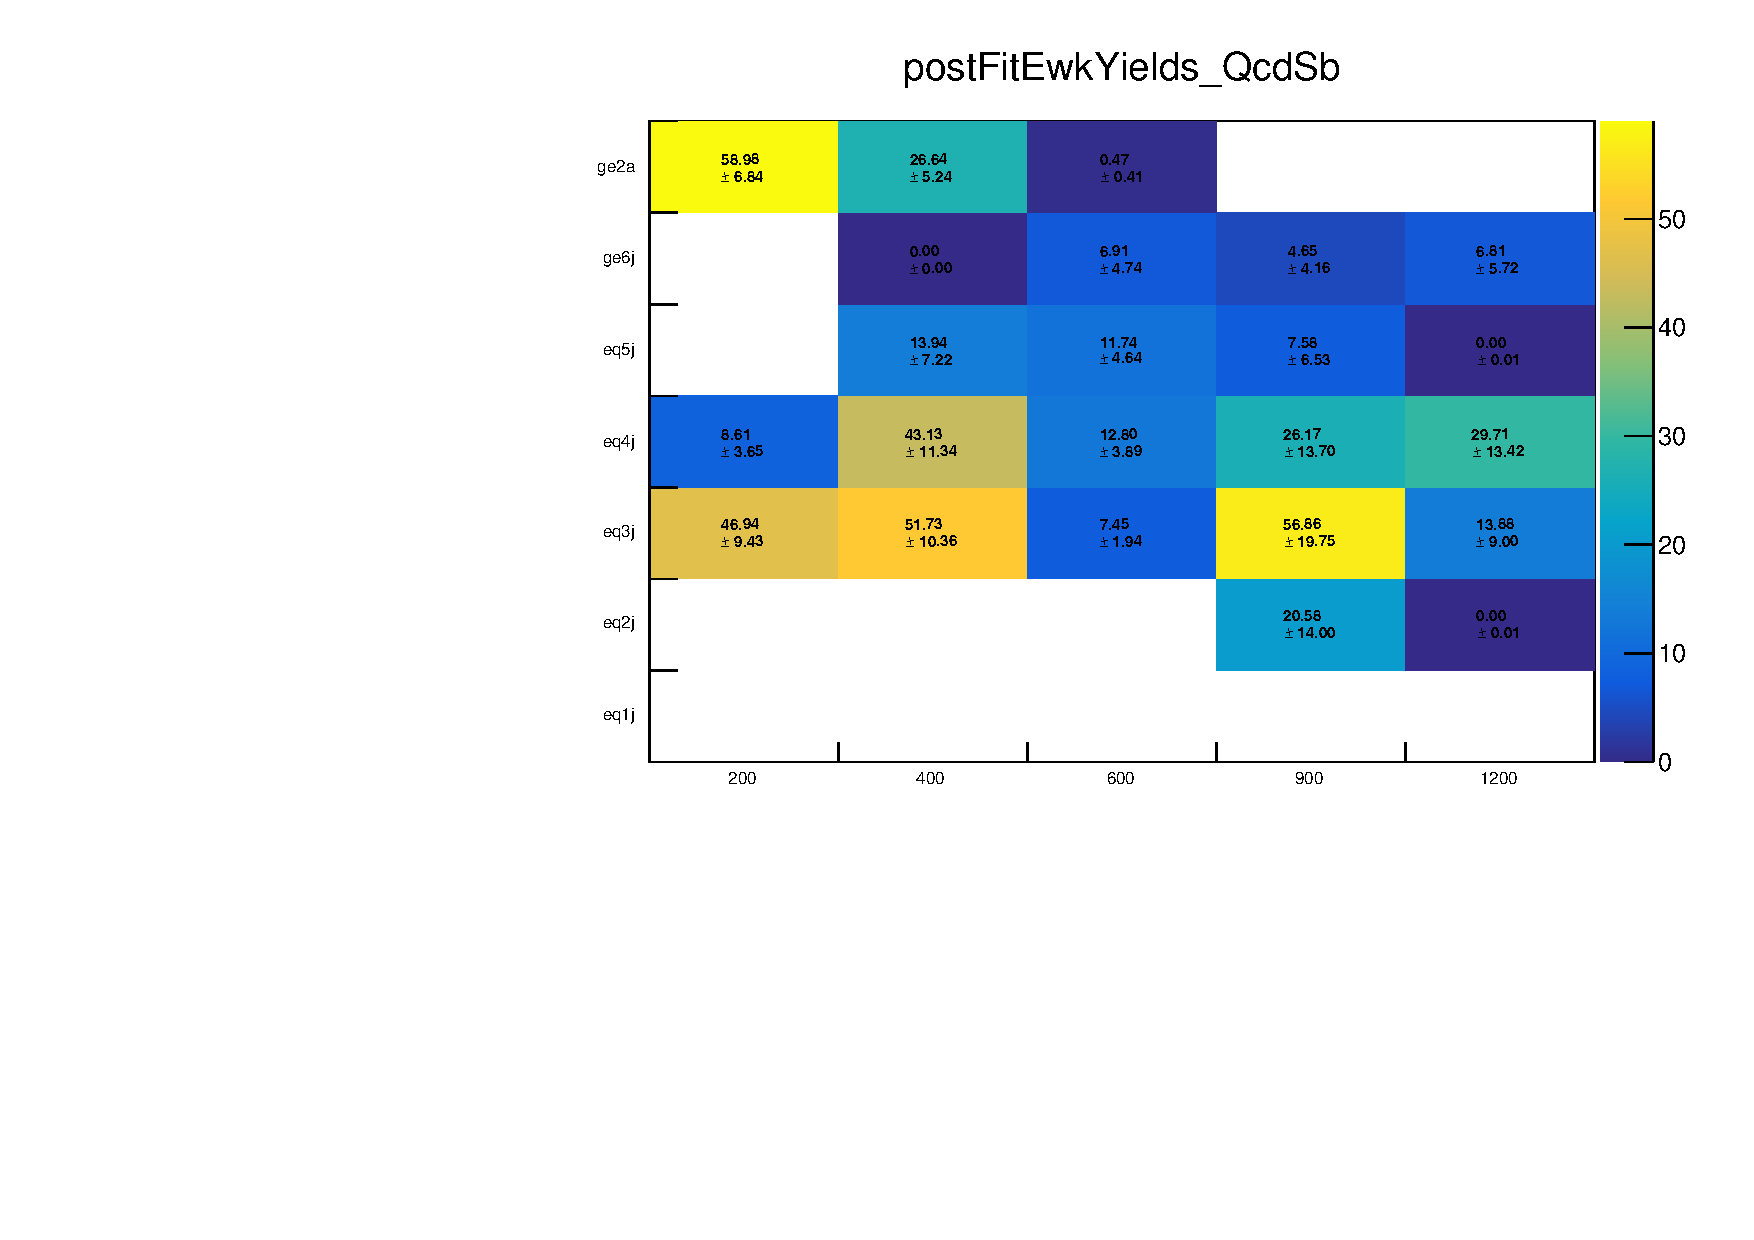
\includegraphics[width=0.5\textwidth]{figures/qcd/qcdANPlotsDoubleSb/postFitEwkYields_QcdSb}
  } \\
  \subfigure[Post-fit constraints on $\mu_{\textrm{QCD}}$.]{
    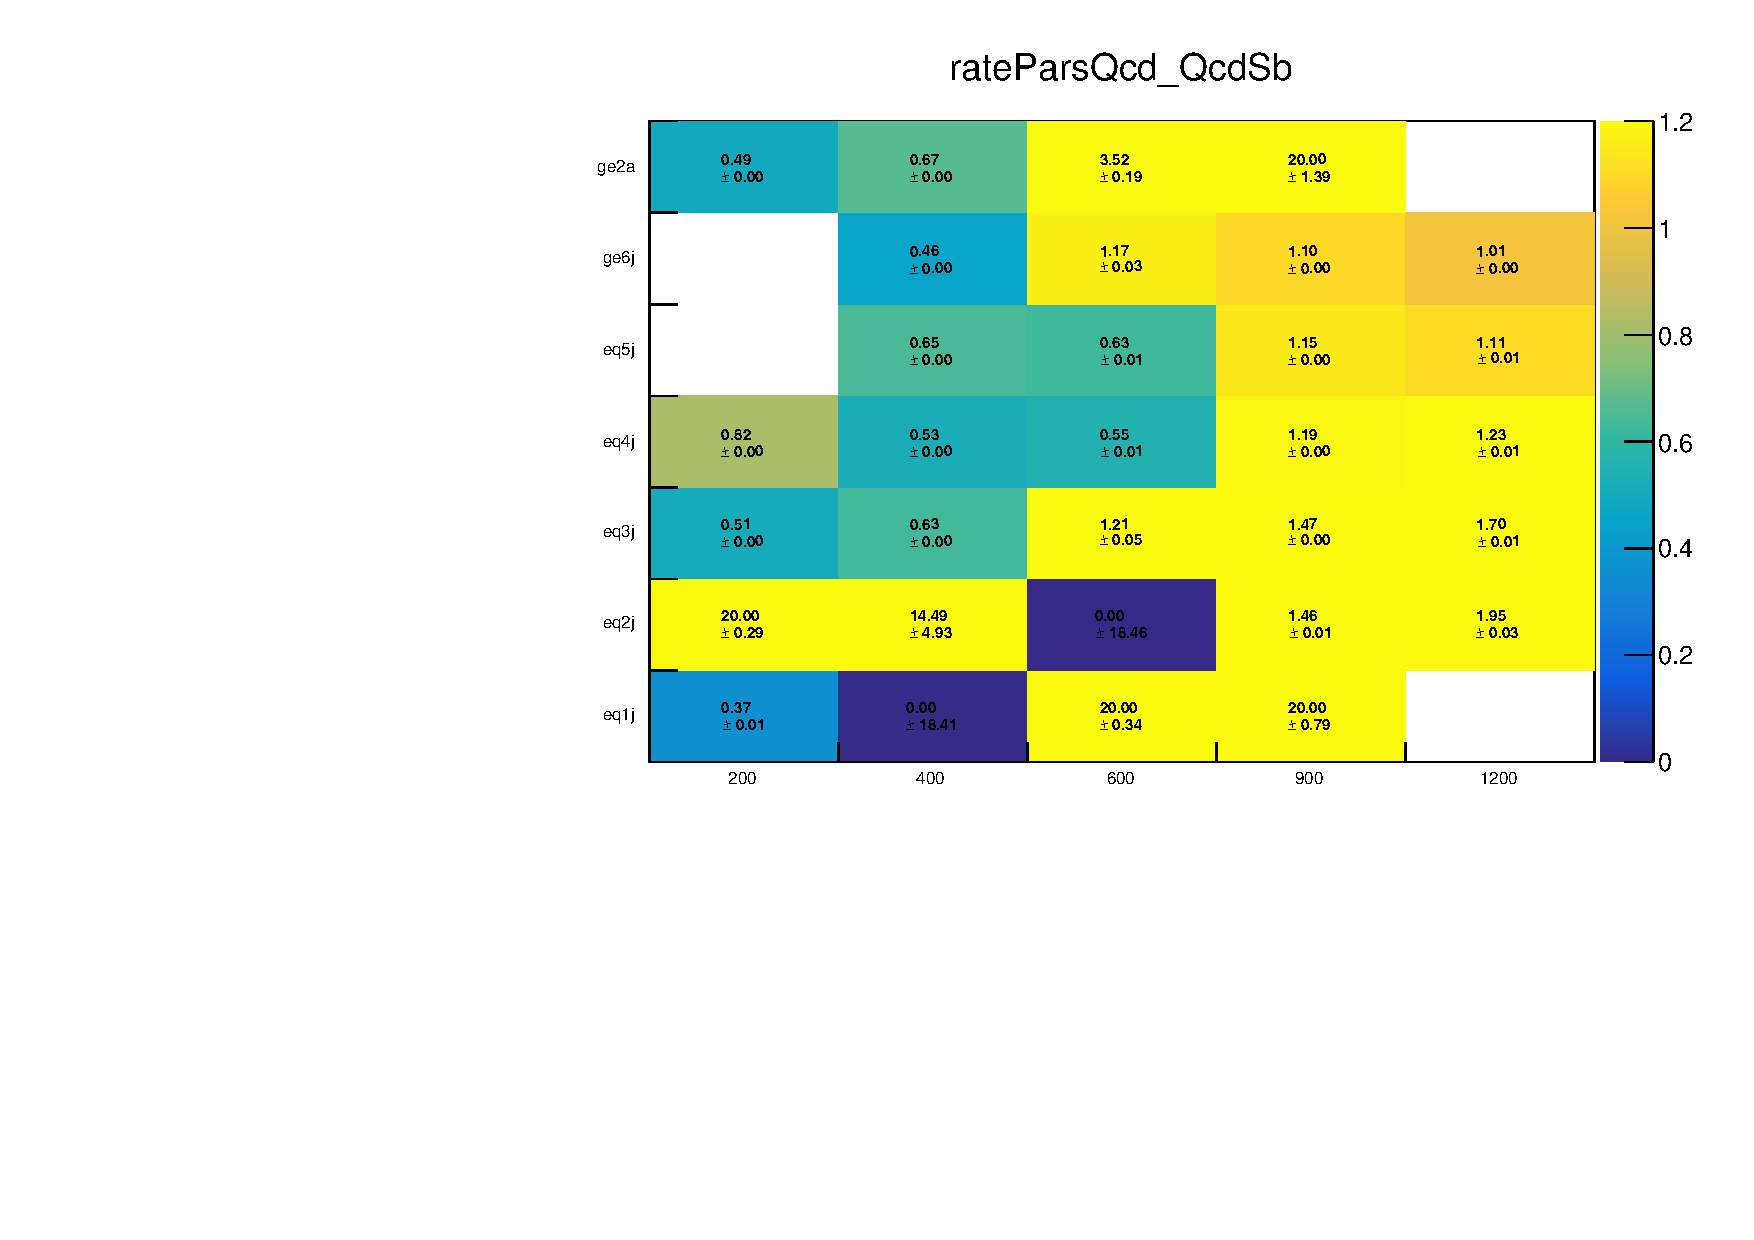
\includegraphics[width=0.5\textwidth]{figures/qcd/qcdANPlotsDoubleSb/rateParsQcd_QcdSb}
  } 
  \subfigure[Post-fit QCD background estimates.]{
    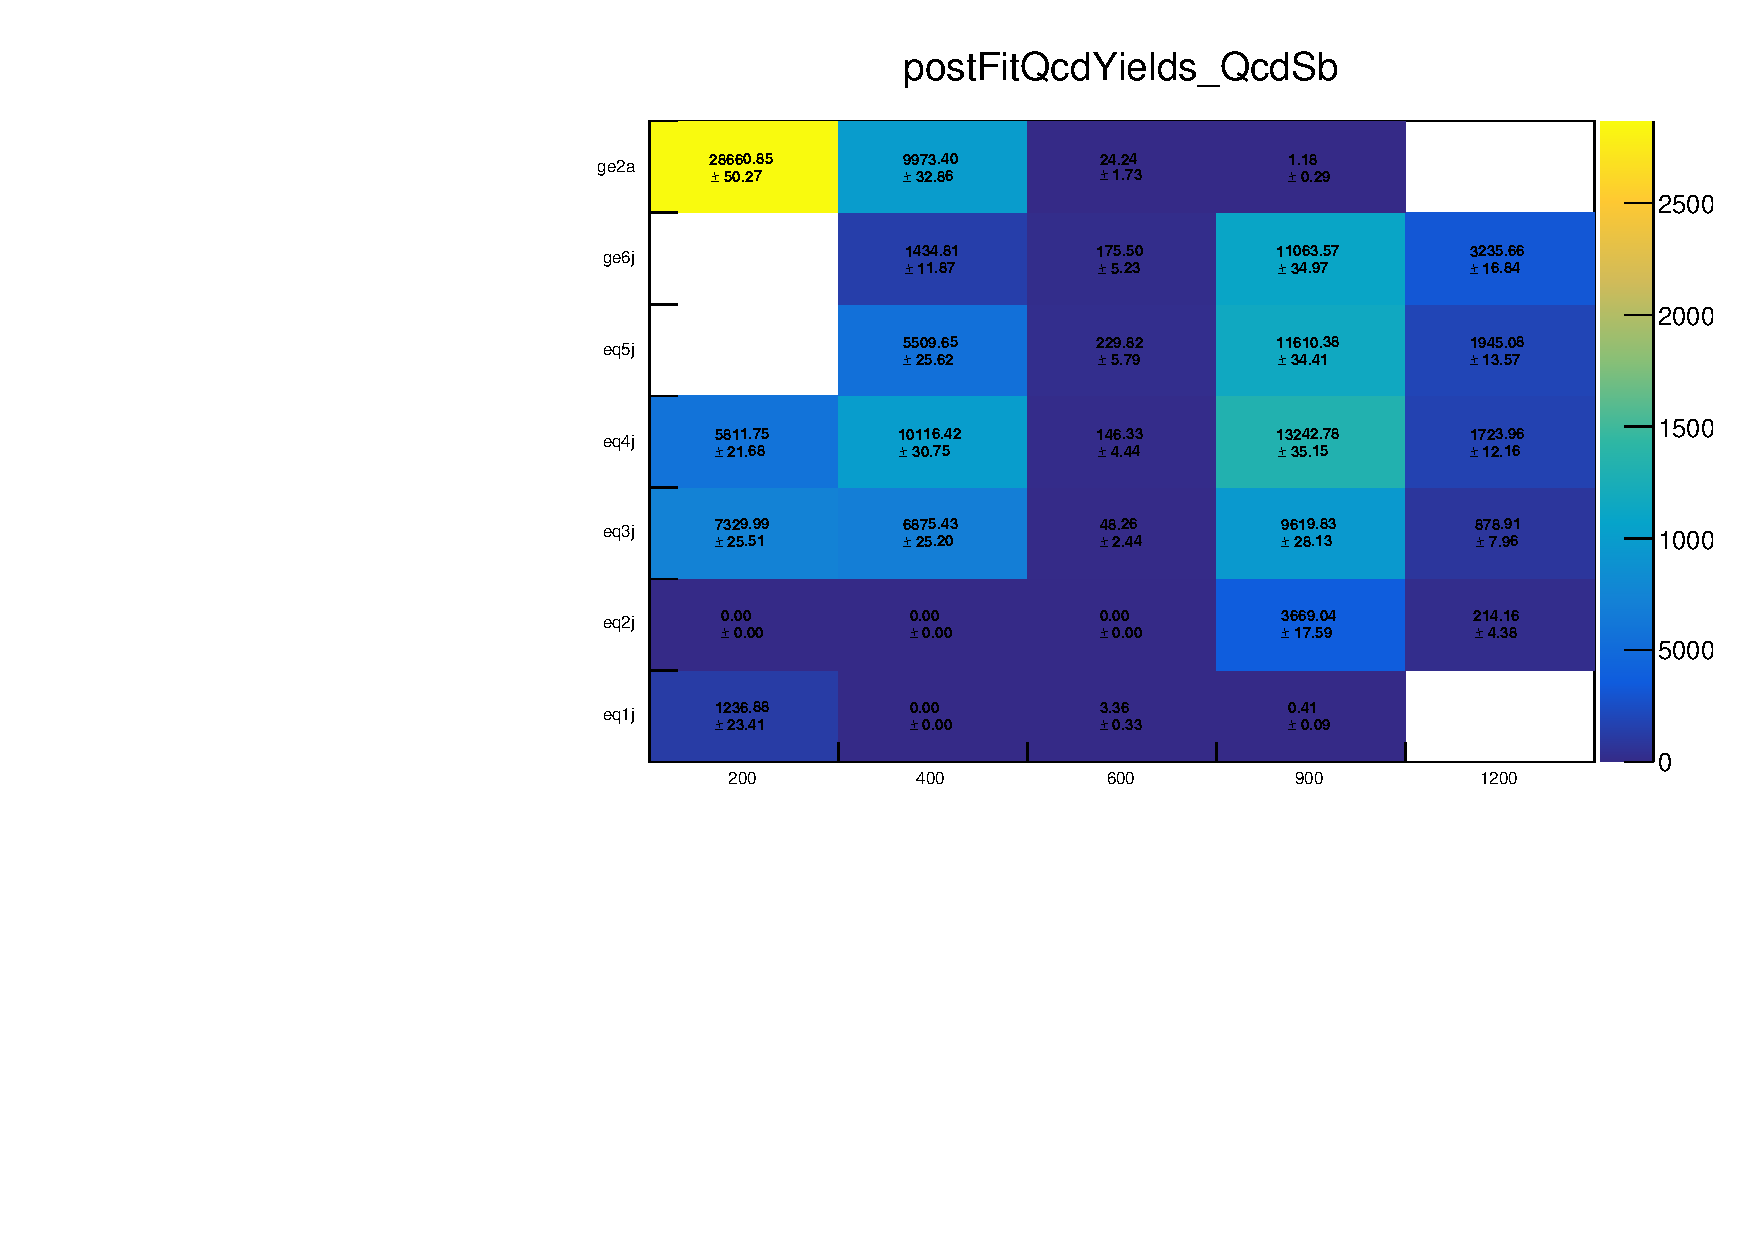
\includegraphics[width=0.5\textwidth]{figures/qcd/qcdANPlotsDoubleSb/postFitQcdYields_QcdSb}
  } \\
  \caption{Data counts, post-fit estimates of the EWK and QCD
    background contributions, and the constrained values of the
    floating parameters $\mu_{\textrm{QCD}}$, in (\njet, \scalht) bins
    of the ``double'' \mhtmet and \bdphi sideband (region ``A'' in Table~\ref{tab:qcd_sidebands}).}
  \label{fig:mhtmet_sideband}
\end{figure}


% MORE INCLUSIVE QCD VALIDATION
% \clearpage
% \begin{figure}[h!]
%   \begin{center}
%     \subfigure[{ Symmetric
%     }]{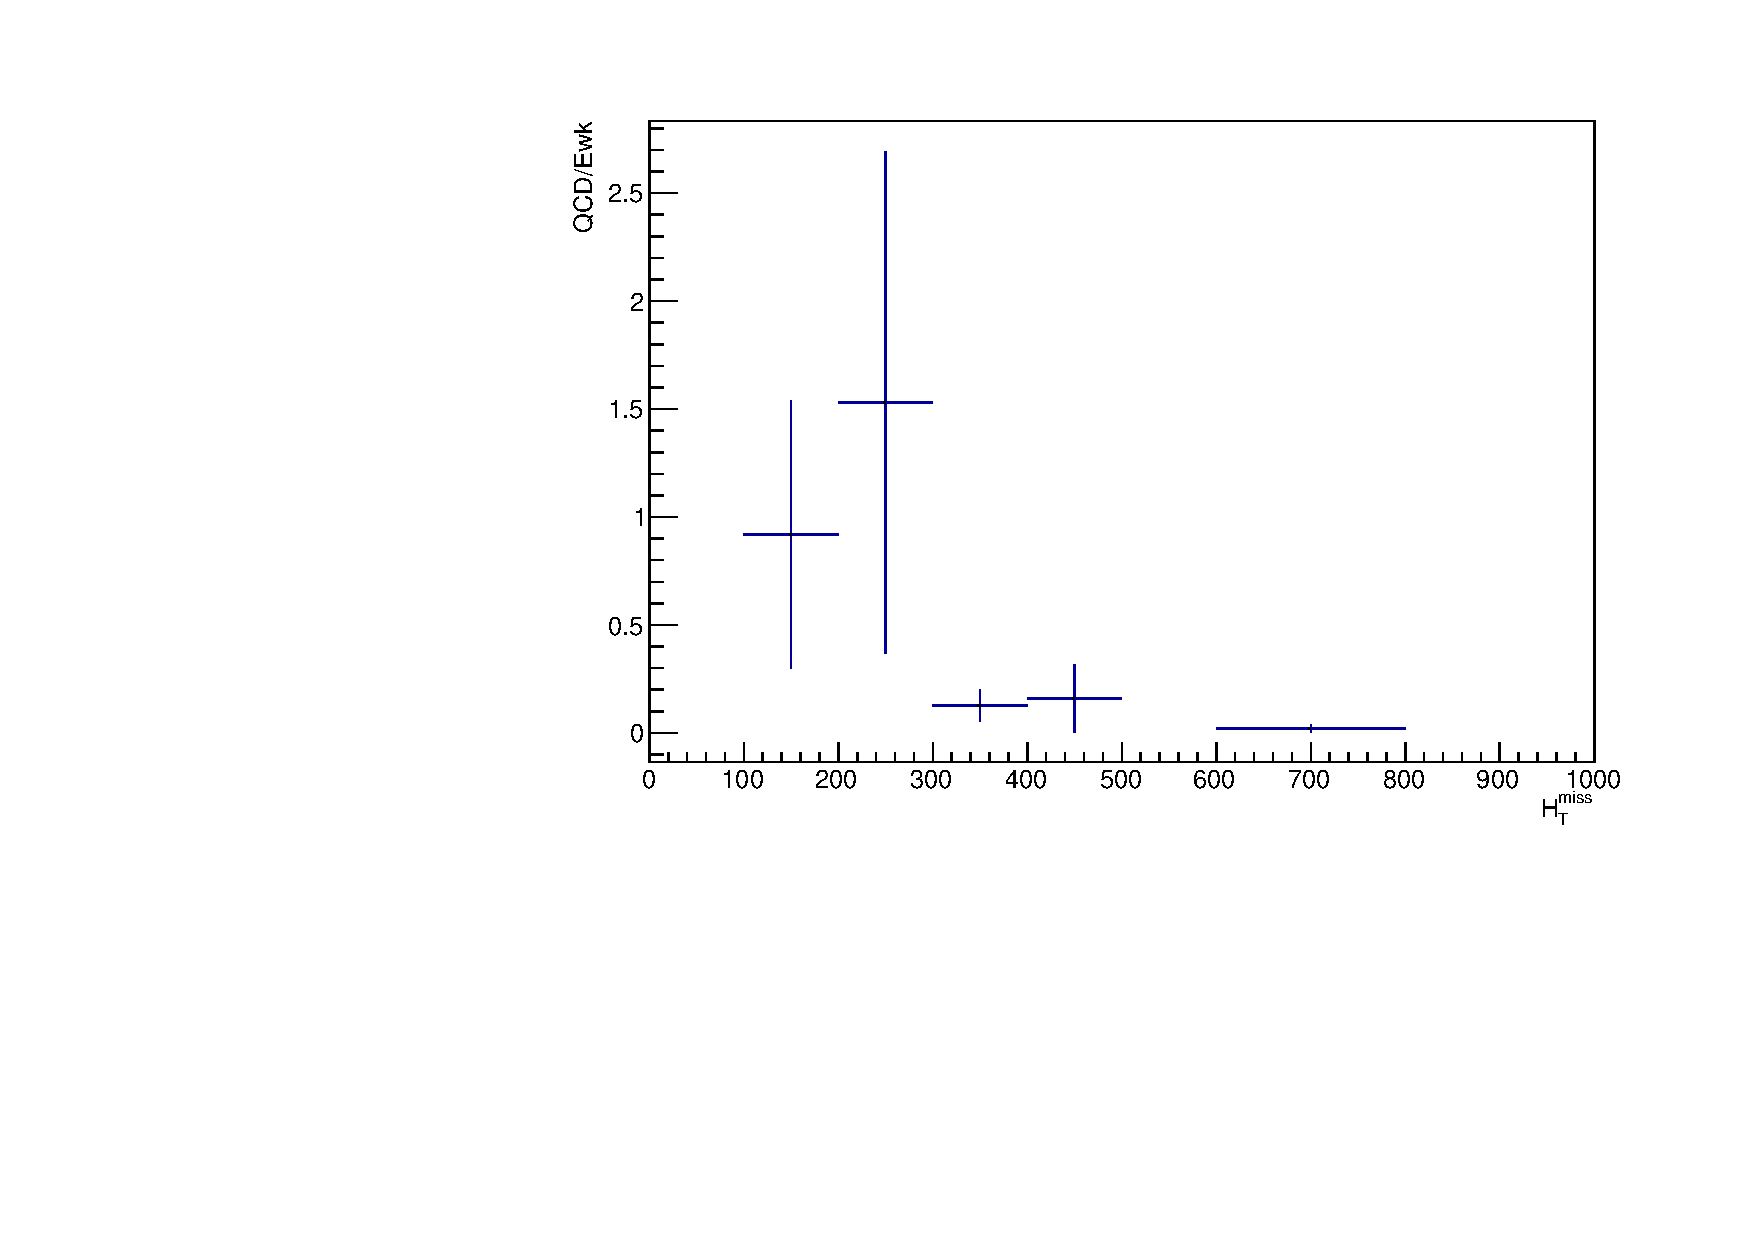
\includegraphics[width=0.5\textwidth]{figures/qcd/mht_ht_allsym}} ~~
%     \subfigure[{ Symmetric
%     }]{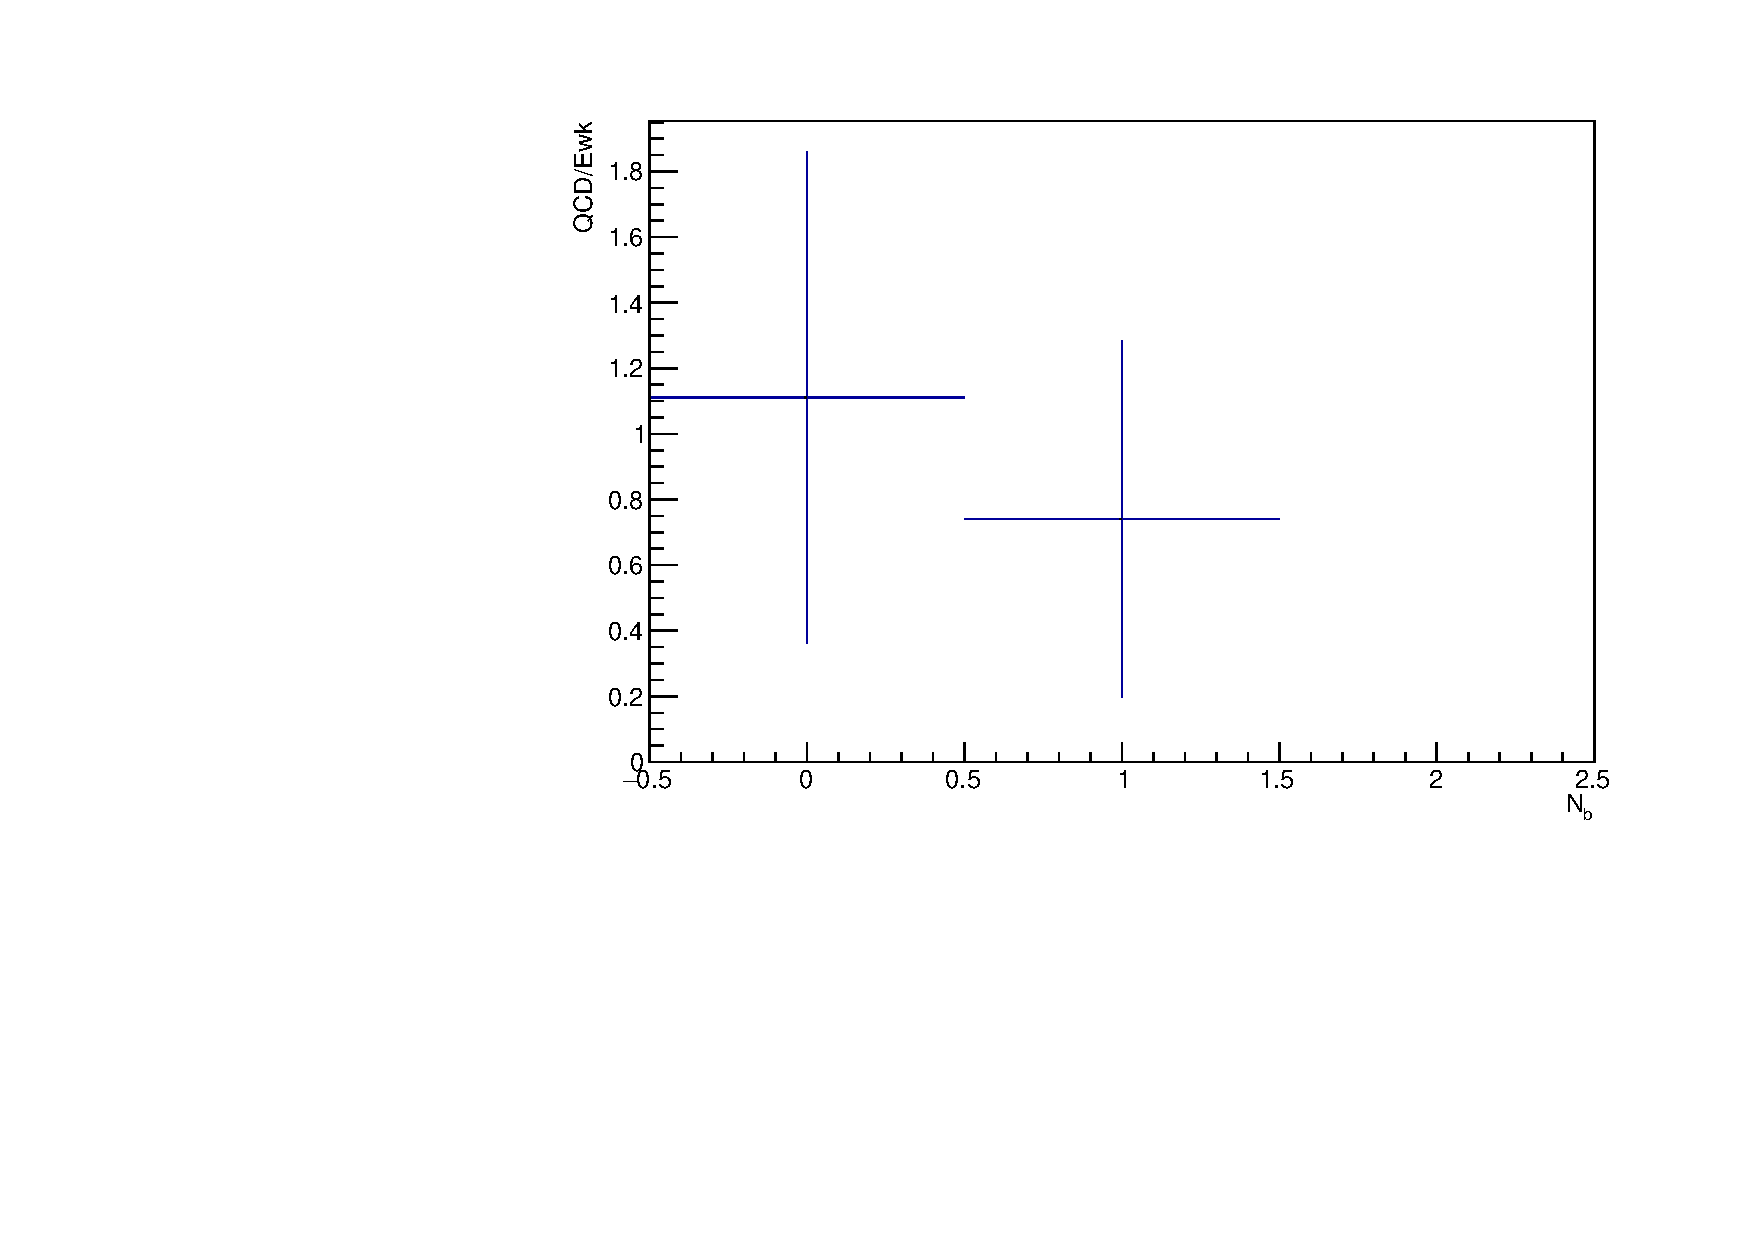
\includegraphics[width=0.5\textwidth]{figures/qcd/nB_ht_allsym}} \\
%     \subfigure[{ Asymmetric
%     }]{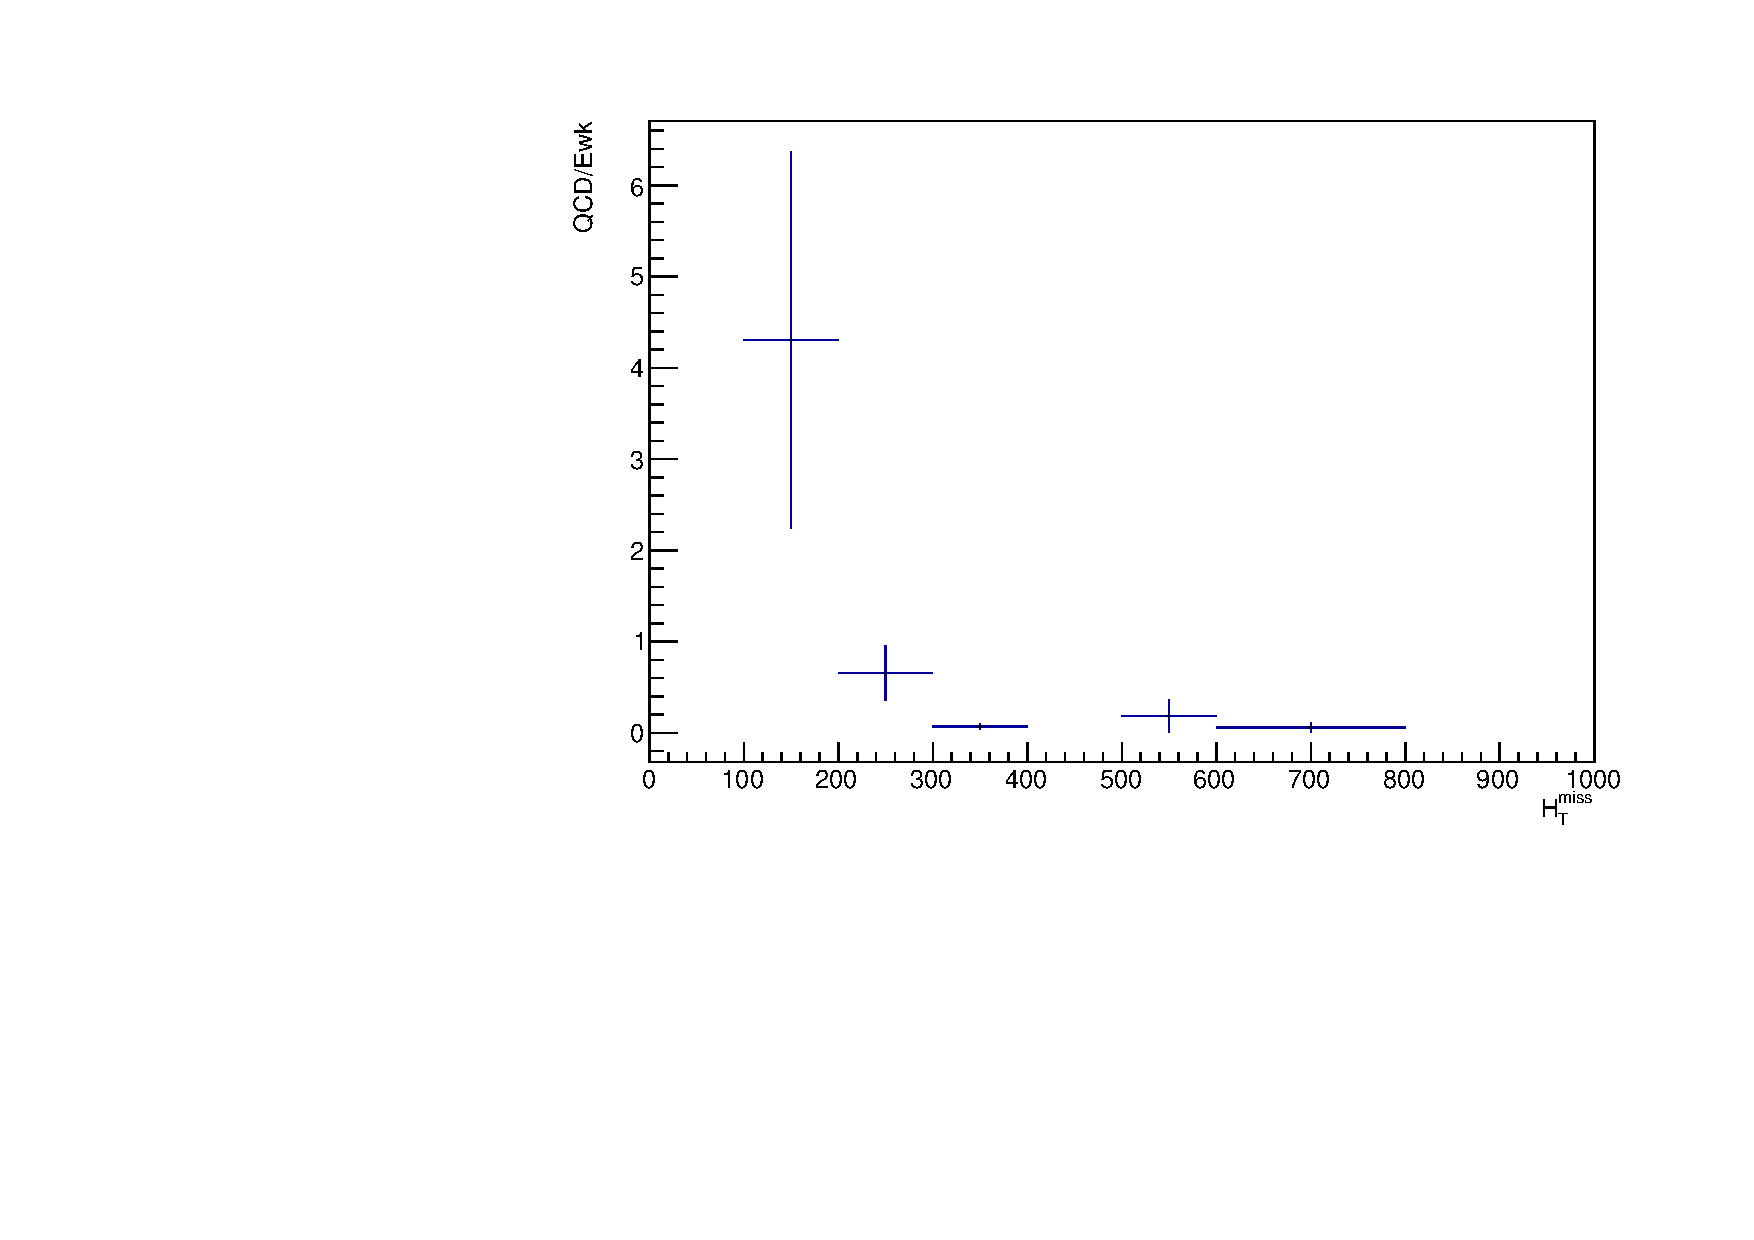
\includegraphics[width=0.5\textwidth]{figures/qcd/mht_ht_allasym}} ~~
%     \subfigure[{ Asymmetric
%     }]{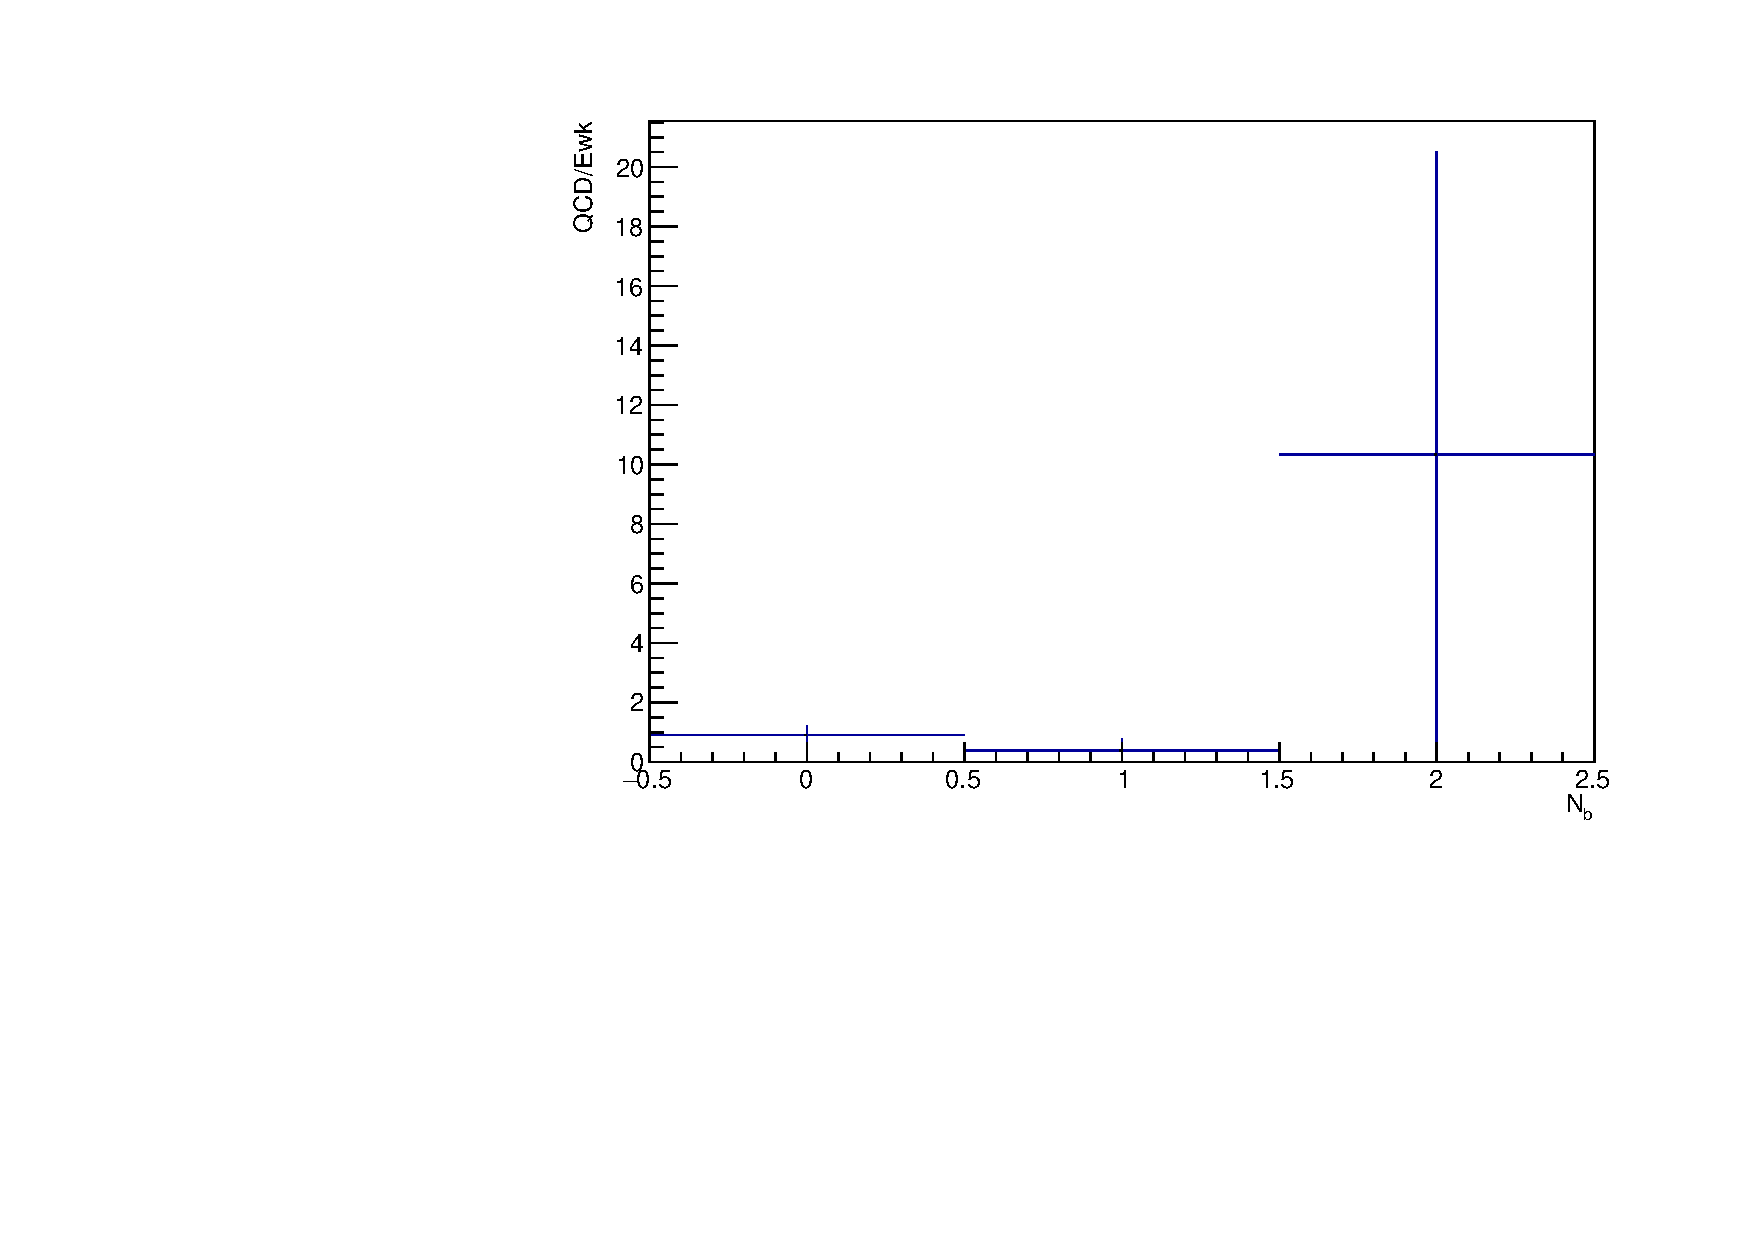
\includegraphics[width=0.5\textwidth]{figures/qcd/nB_ht_allasym}} \\
%     \caption{ Ratio of QCD to EWK Monte Carlo prediction in
%     the signal region for different jet topologies a function
%     of \mht (Left) and $\nb$ (Right).
%     %A constant fit to the data is represented by the red line, with the $\pm$100\% uncertainty represented by the blue hashed region.
%     }
%     \label{fig:qcd_validation}
%   \end{center} 
% \end{figure}


% LESS INCLUSIVE QCD VALIDATION
% \clearpage
% \begin{figure}[h!]
%   \begin{center}
%     \subfigure[{ Asymmetric,
%     $\scalht<400$~GeV}]{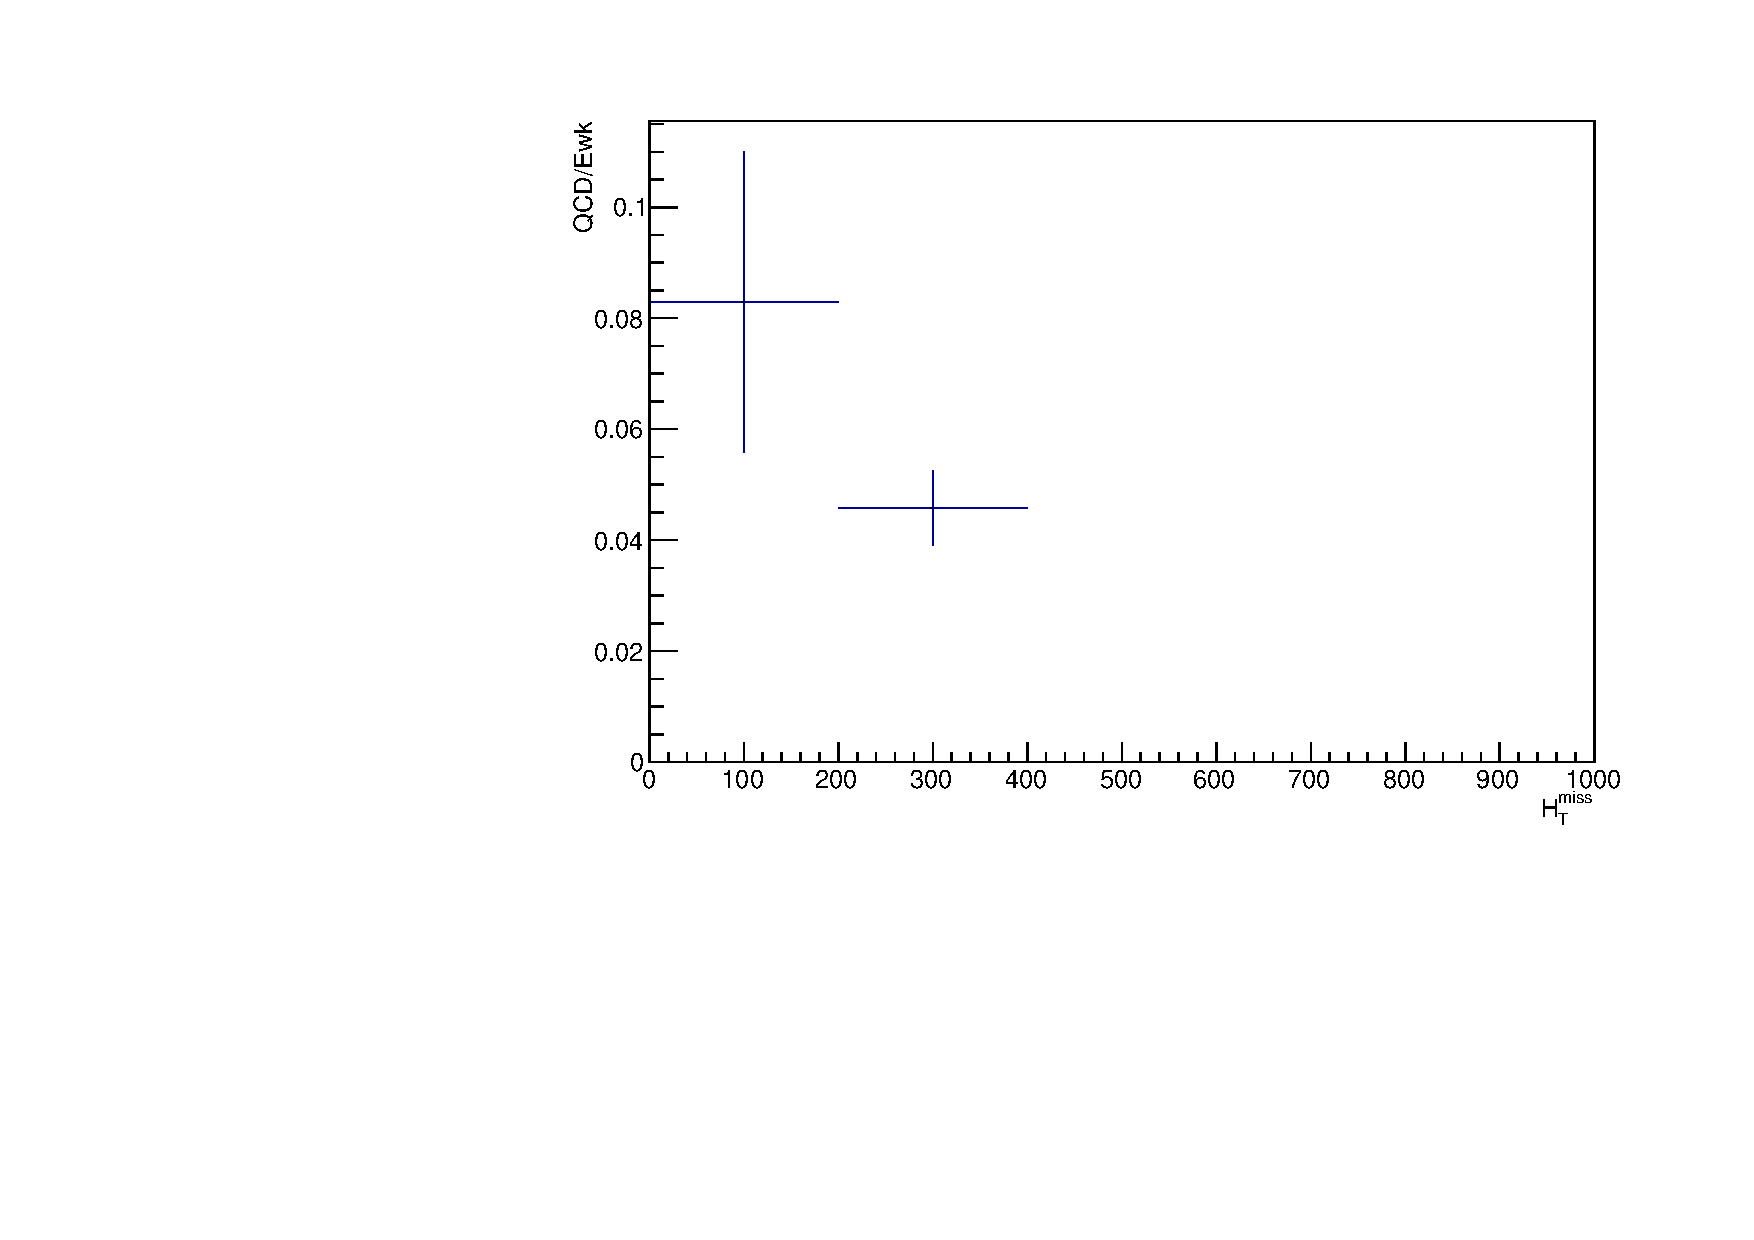
\includegraphics[width=0.5\textwidth]{figures/qcd/plots/mht_ht_lt400asym}} ~~
%     \subfigure[{ Asymmetric,
%     $\scalht<400$~GeV}]{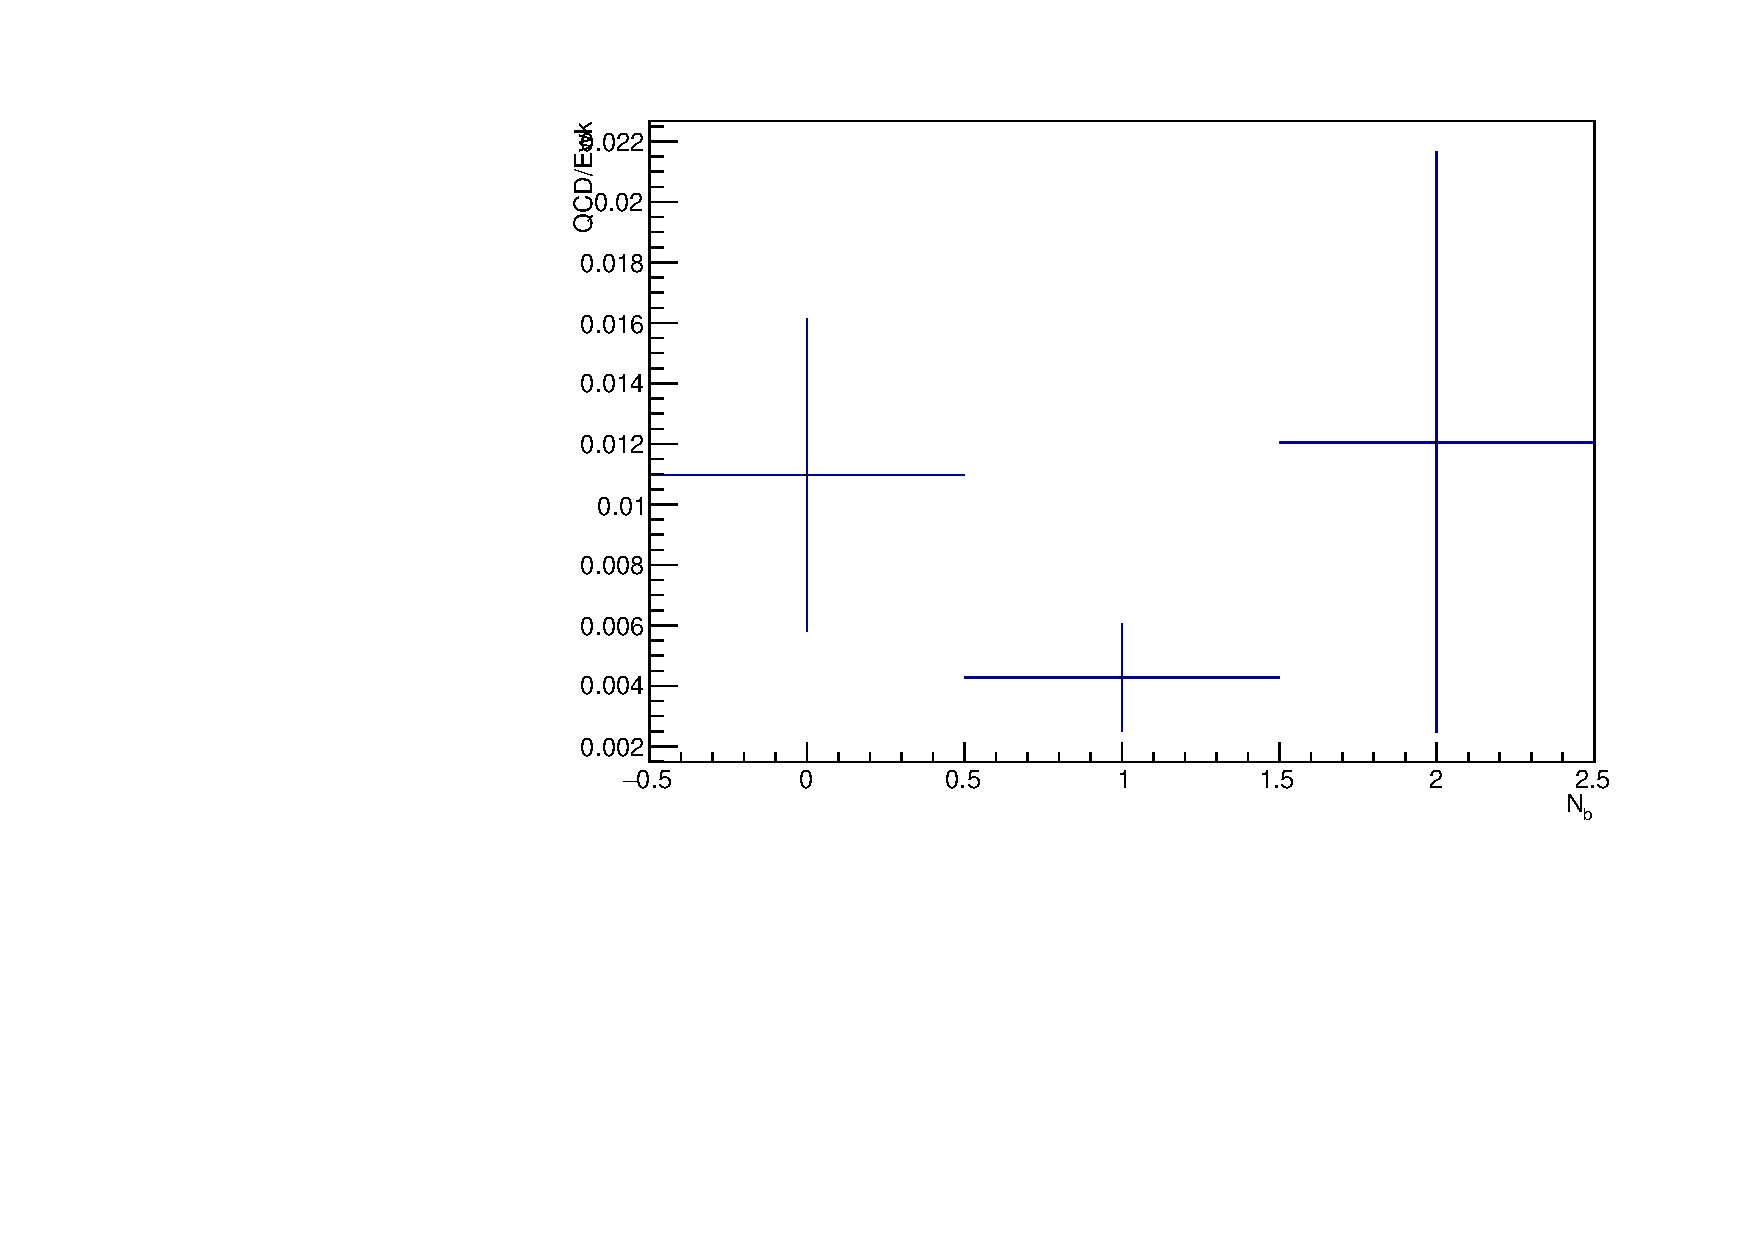
\includegraphics[width=0.5\textwidth]{figures/qcd/plots/nB_ht_lt400asym}} \\
%     \subfigure[{ Asymmetric,
%     $400<\scalht<800$~GeV}]{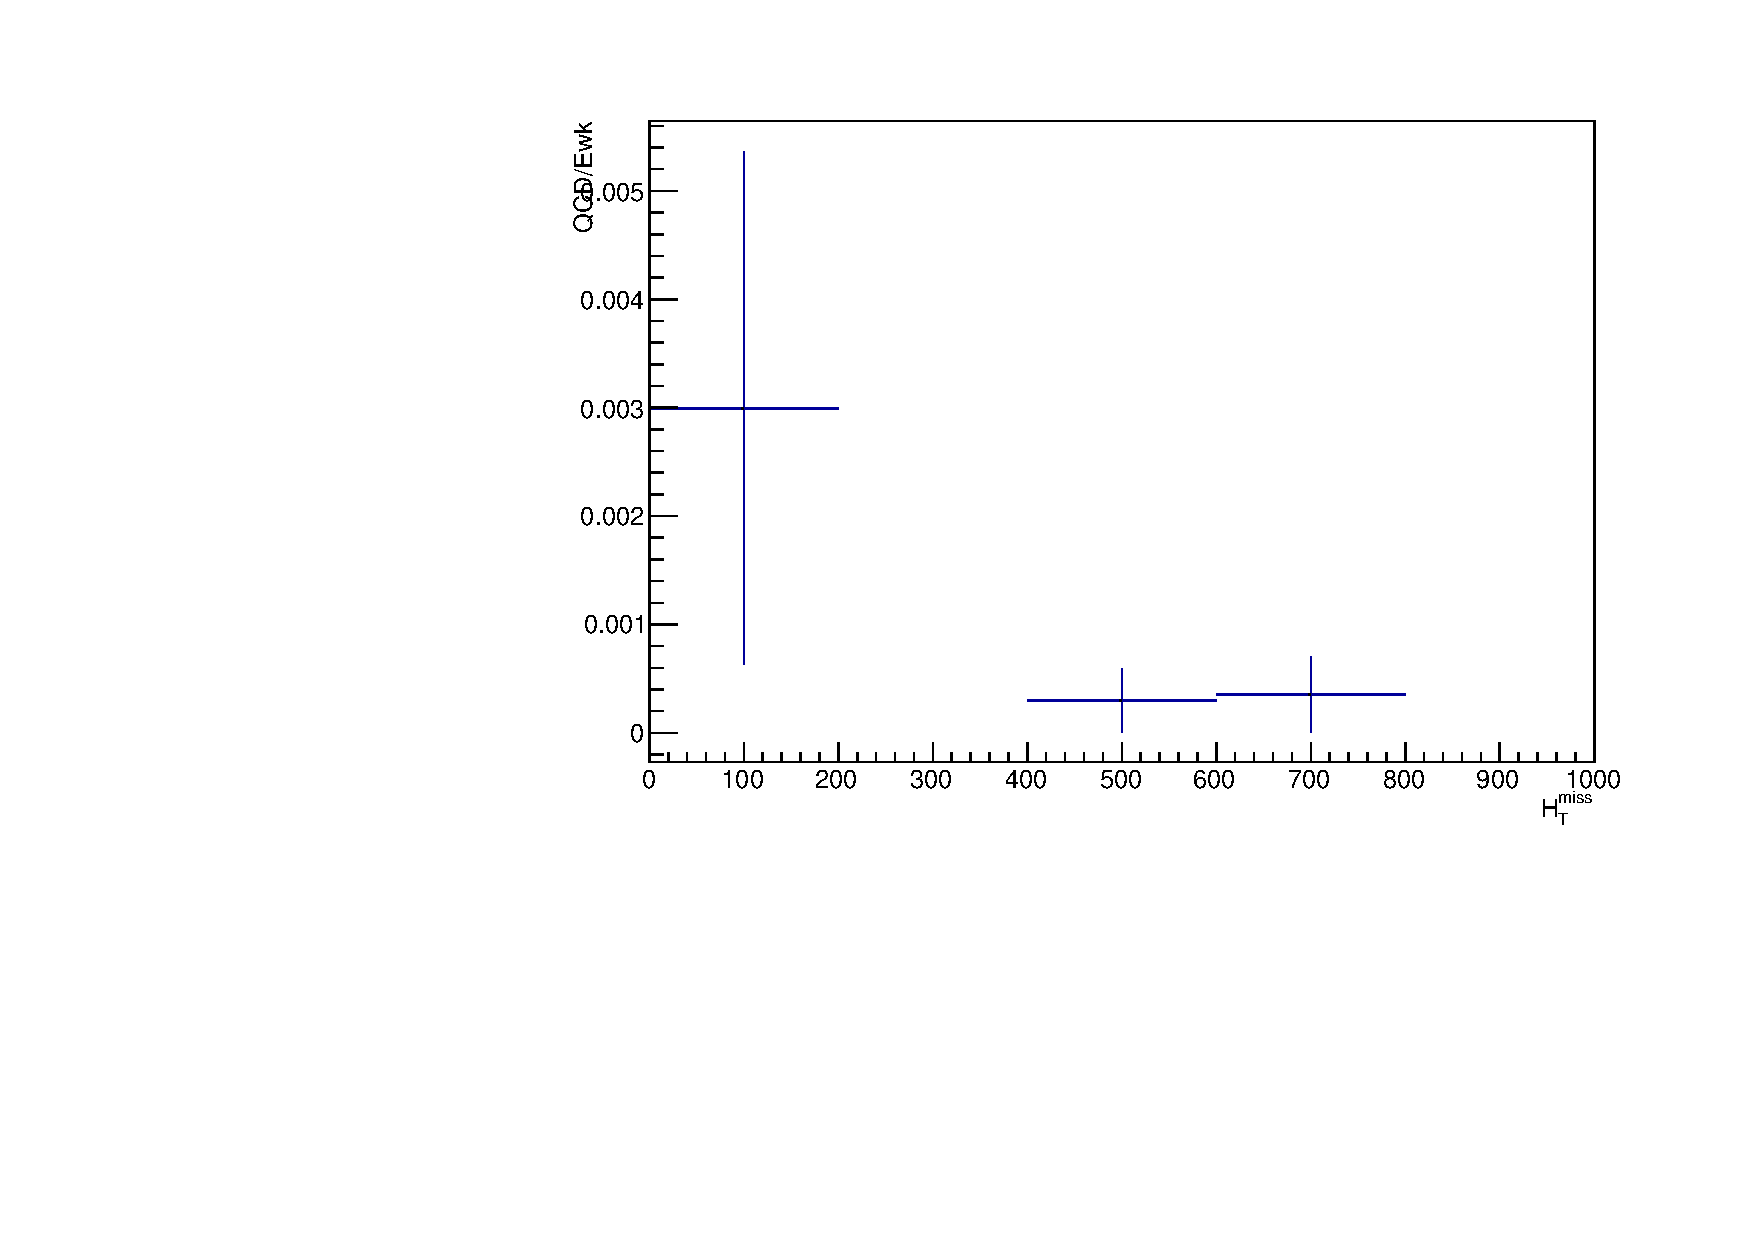
\includegraphics[width=0.5\textwidth]{figures/qcd/plots/mht_ht_lt800asym}} ~~
%     \subfigure[{ Asymmetric,
%     $400<\scalht<800$~GeV}]{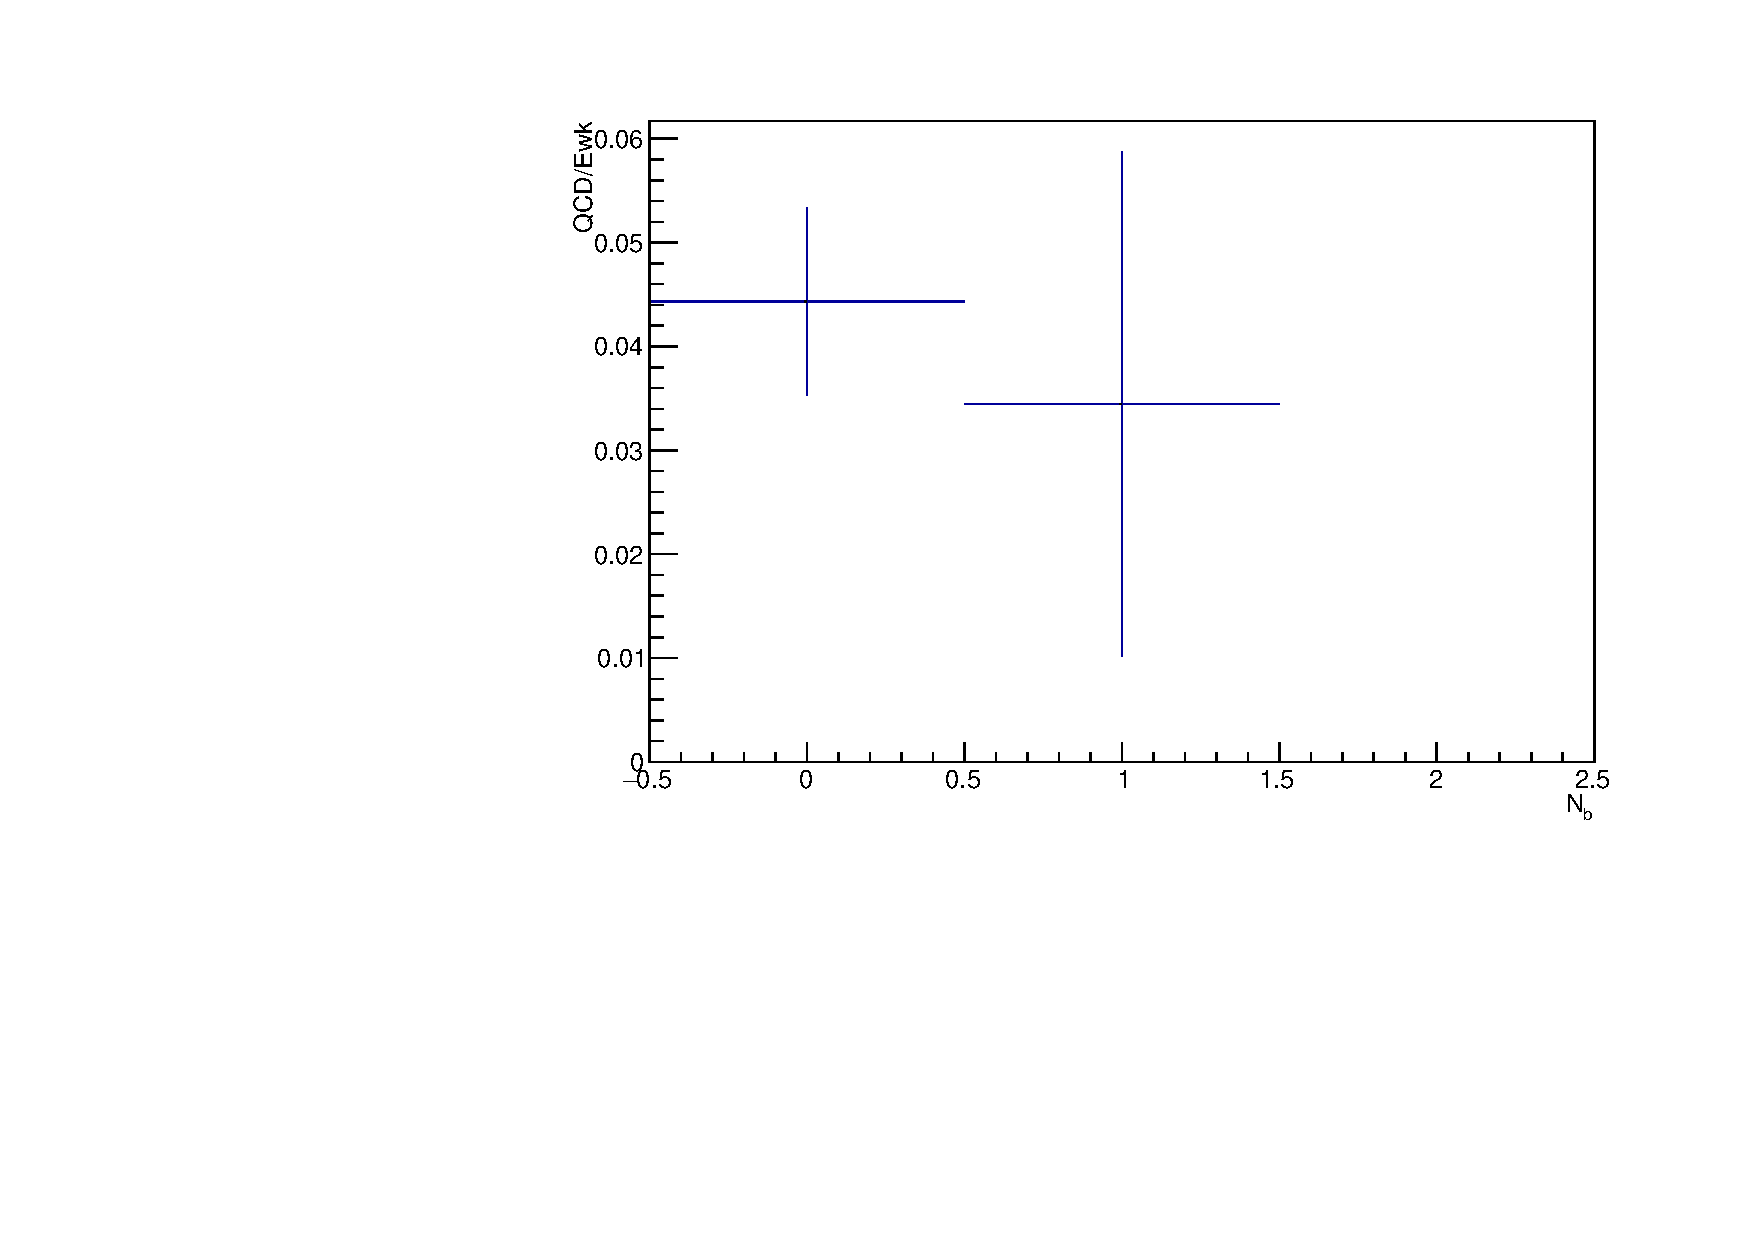
\includegraphics[width=0.5\textwidth]{figures/qcd/plots/nB_ht_lt800asym}} \\
%     \caption{ Ratio of QCD to EWK Monte Carlo prediction in
%     the signal region for different \scalht selections as a function
%     of \mht (Left) and $\nb$ (Right) for the asymmetric jet category.
%     %A constant fit to the data is represented by the red line, with the $\pm$100\% uncertainty represented by the blue hashed region.
%     }
%     \label{fig:asym_qcd_validation}
%   \end{center} 
% \end{figure}
%
% \clearpage
% \begin{figure}[h!]
%   \begin{center}
%     \subfigure[{ Symmetric,
%     $\scalht<400$~GeV}]{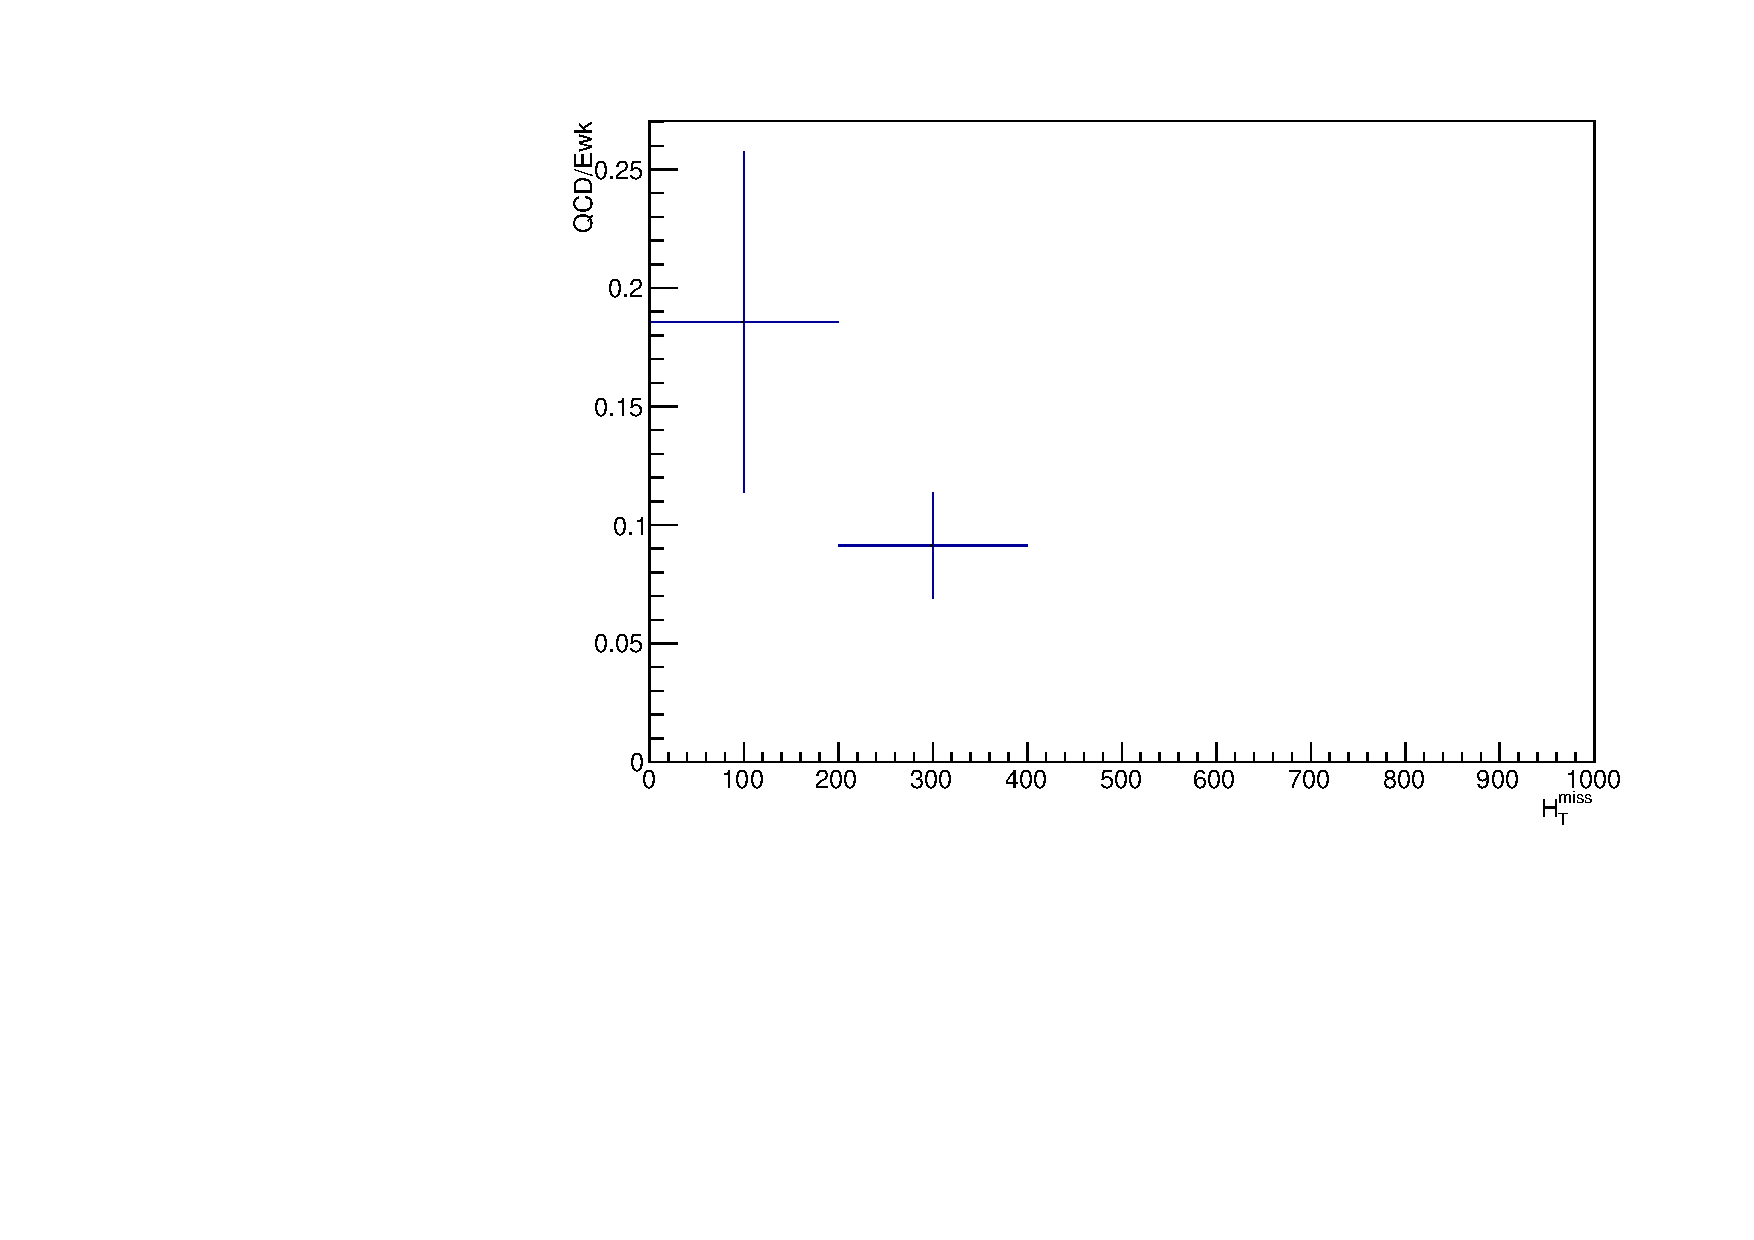
\includegraphics[width=0.5\textwidth]{figures/qcd/plots/mht_ht_lt400sym}} ~~
%     \subfigure[{ Symmetric,
%     $\scalht<400$~GeV}]{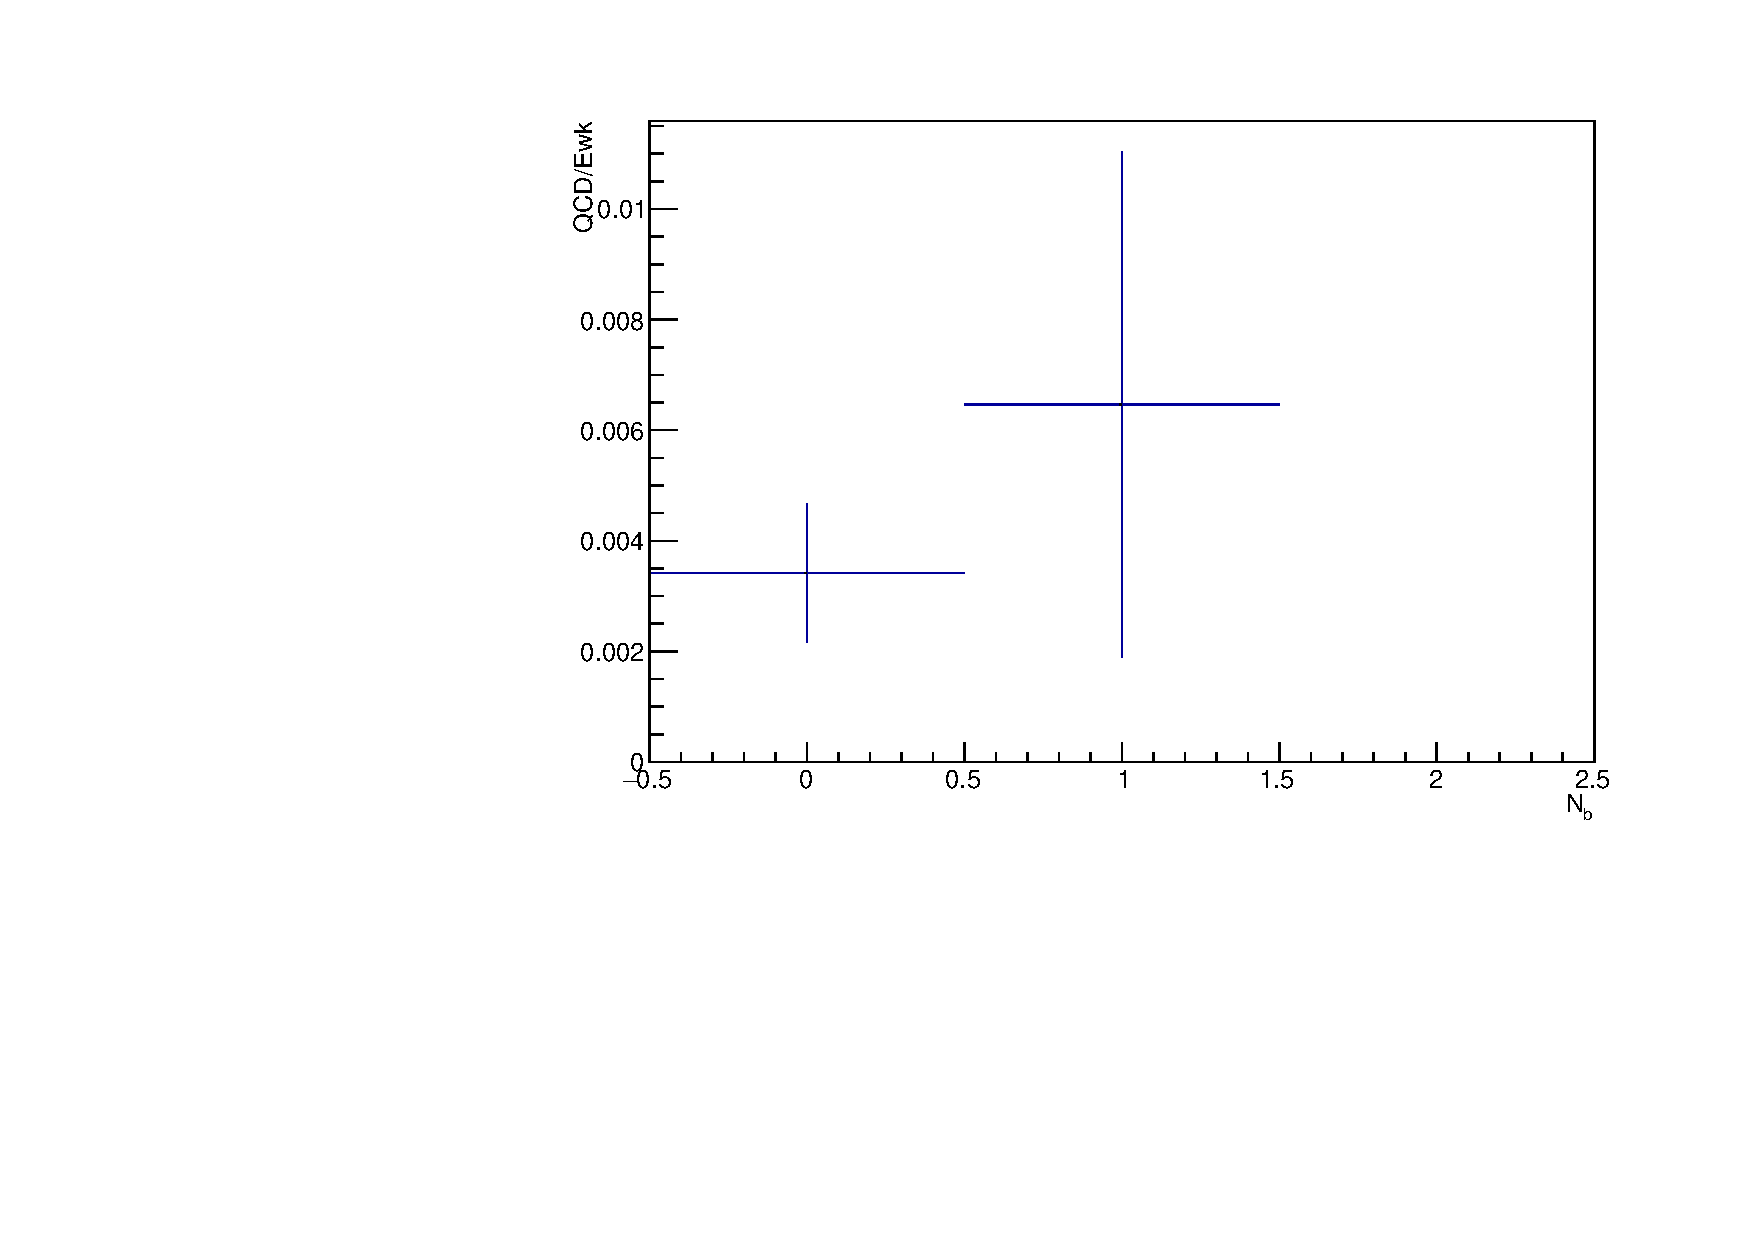
\includegraphics[width=0.5\textwidth]{figures/qcd/plots/nB_ht_lt400sym}} \\
%     \subfigure[{ Symmetric,
%     $400<\scalht>800$~GeV}]{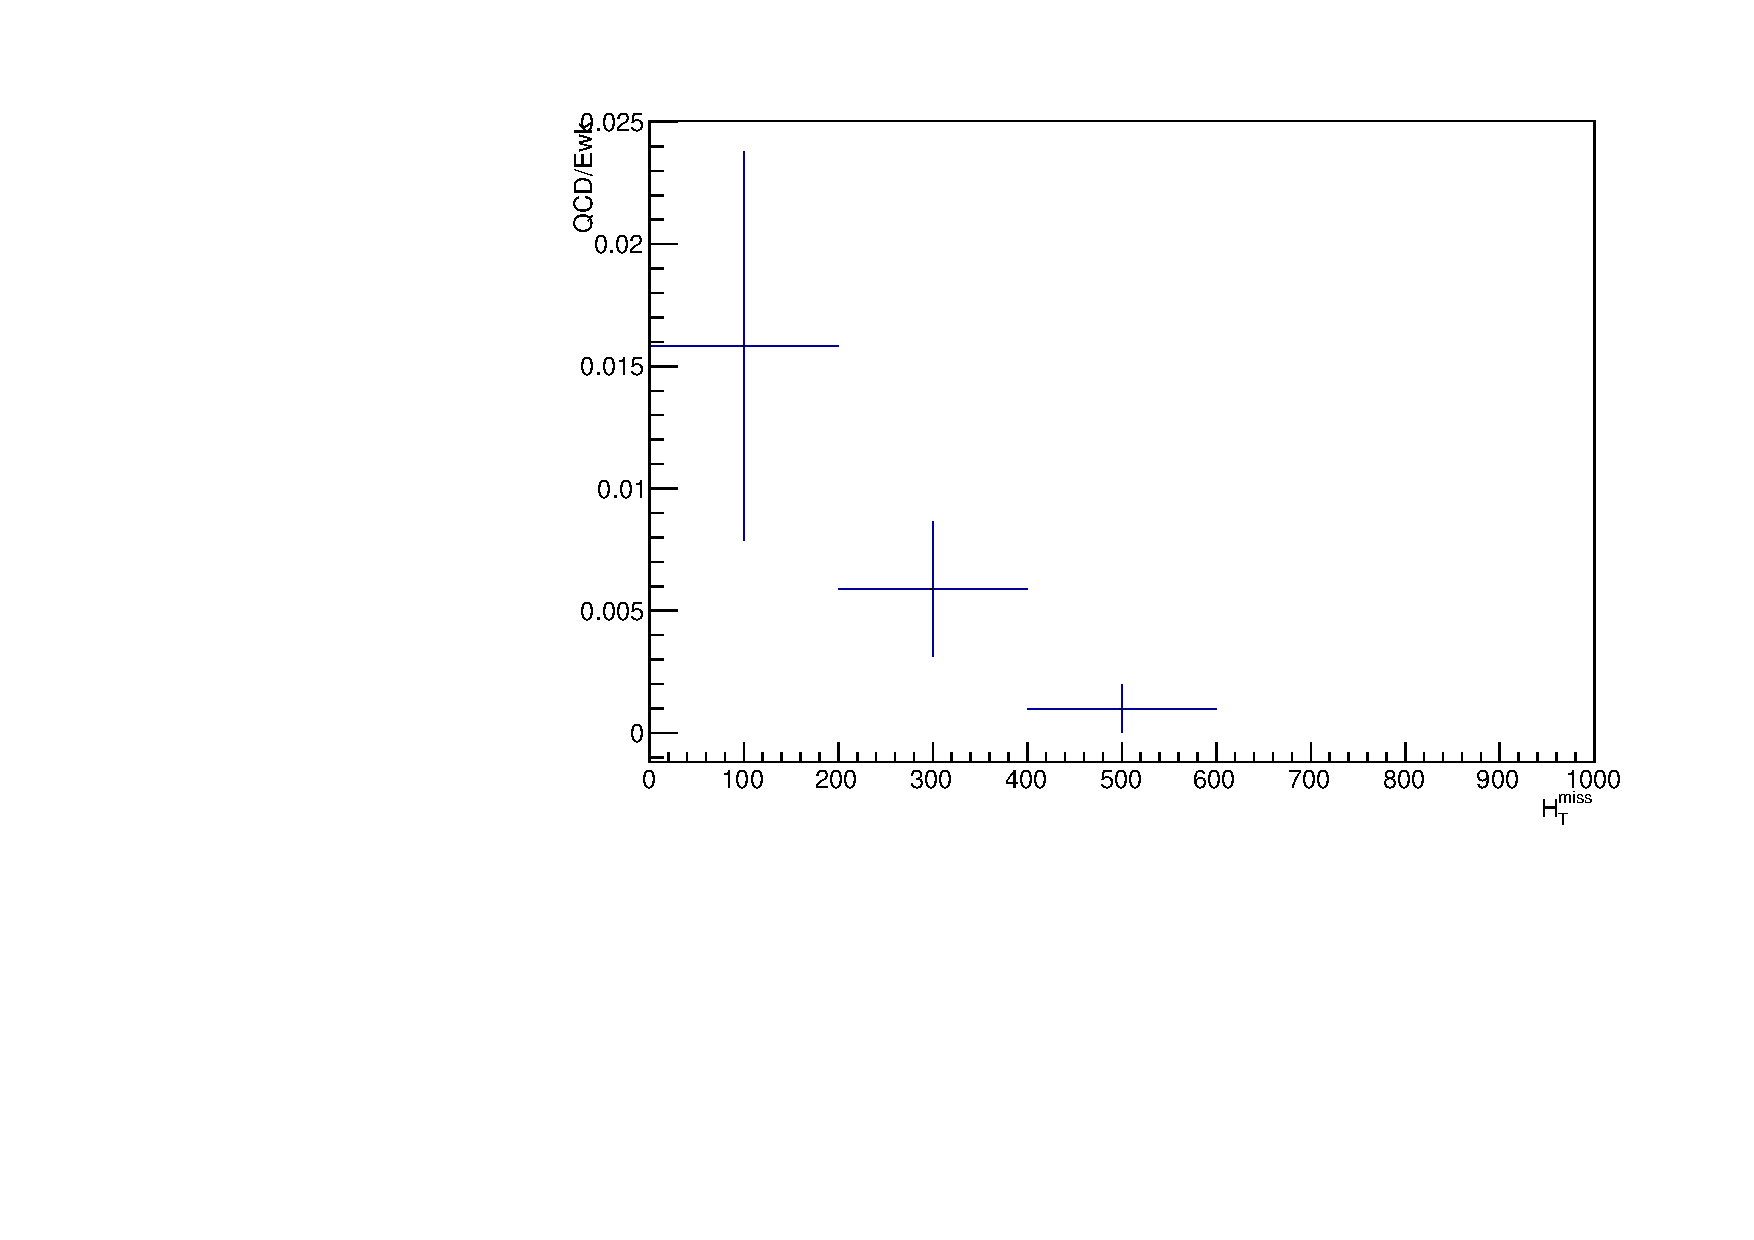
\includegraphics[width=0.5\textwidth]{figures/qcd/plots/mht_ht_lt800sym}} ~~
%     \subfigure[{ Symmetric,
%     $400<\scalht<800$~GeV}]{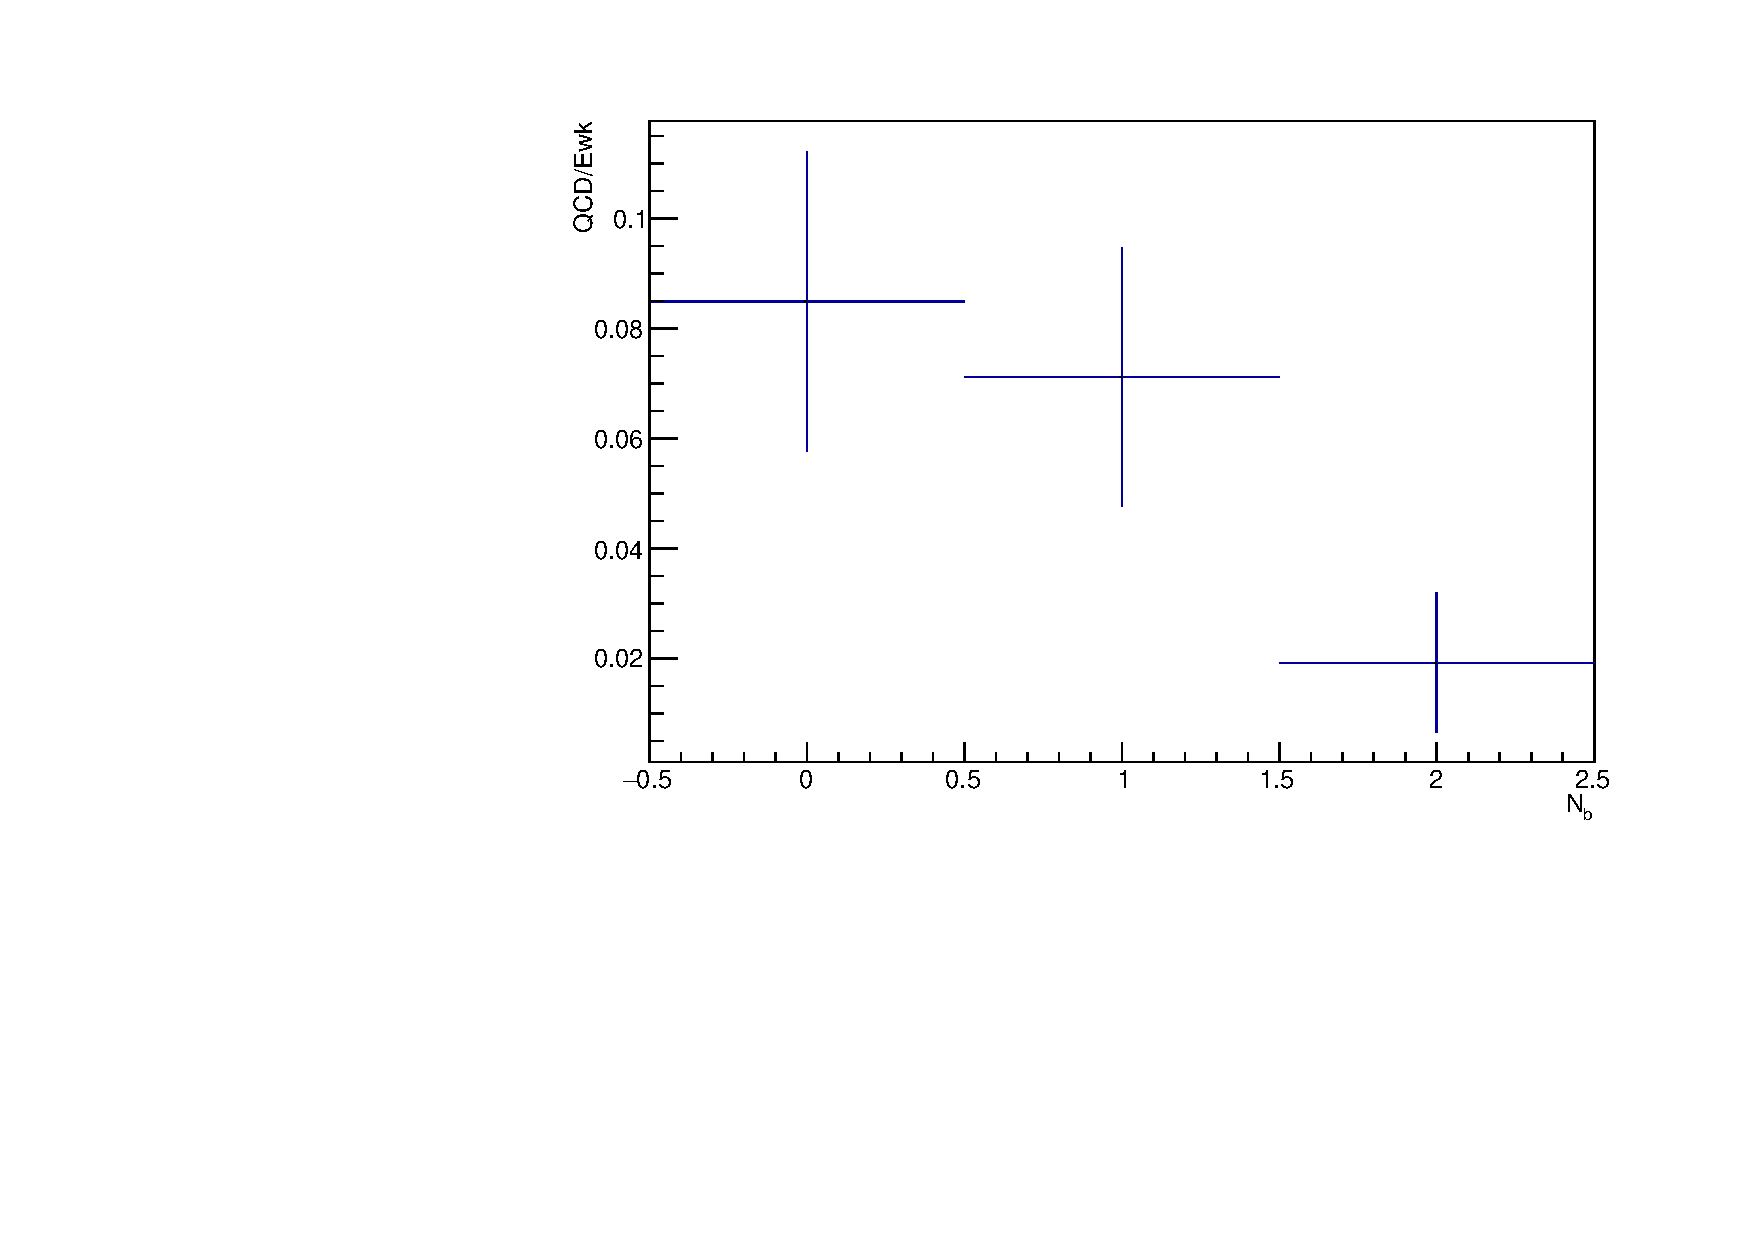
\includegraphics[width=0.5\textwidth]{figures/qcd/plots/nB_ht_lt800sym}} \\
%     \subfigure[{ Symmetric,
%     $\scalht>800$~GeV}]{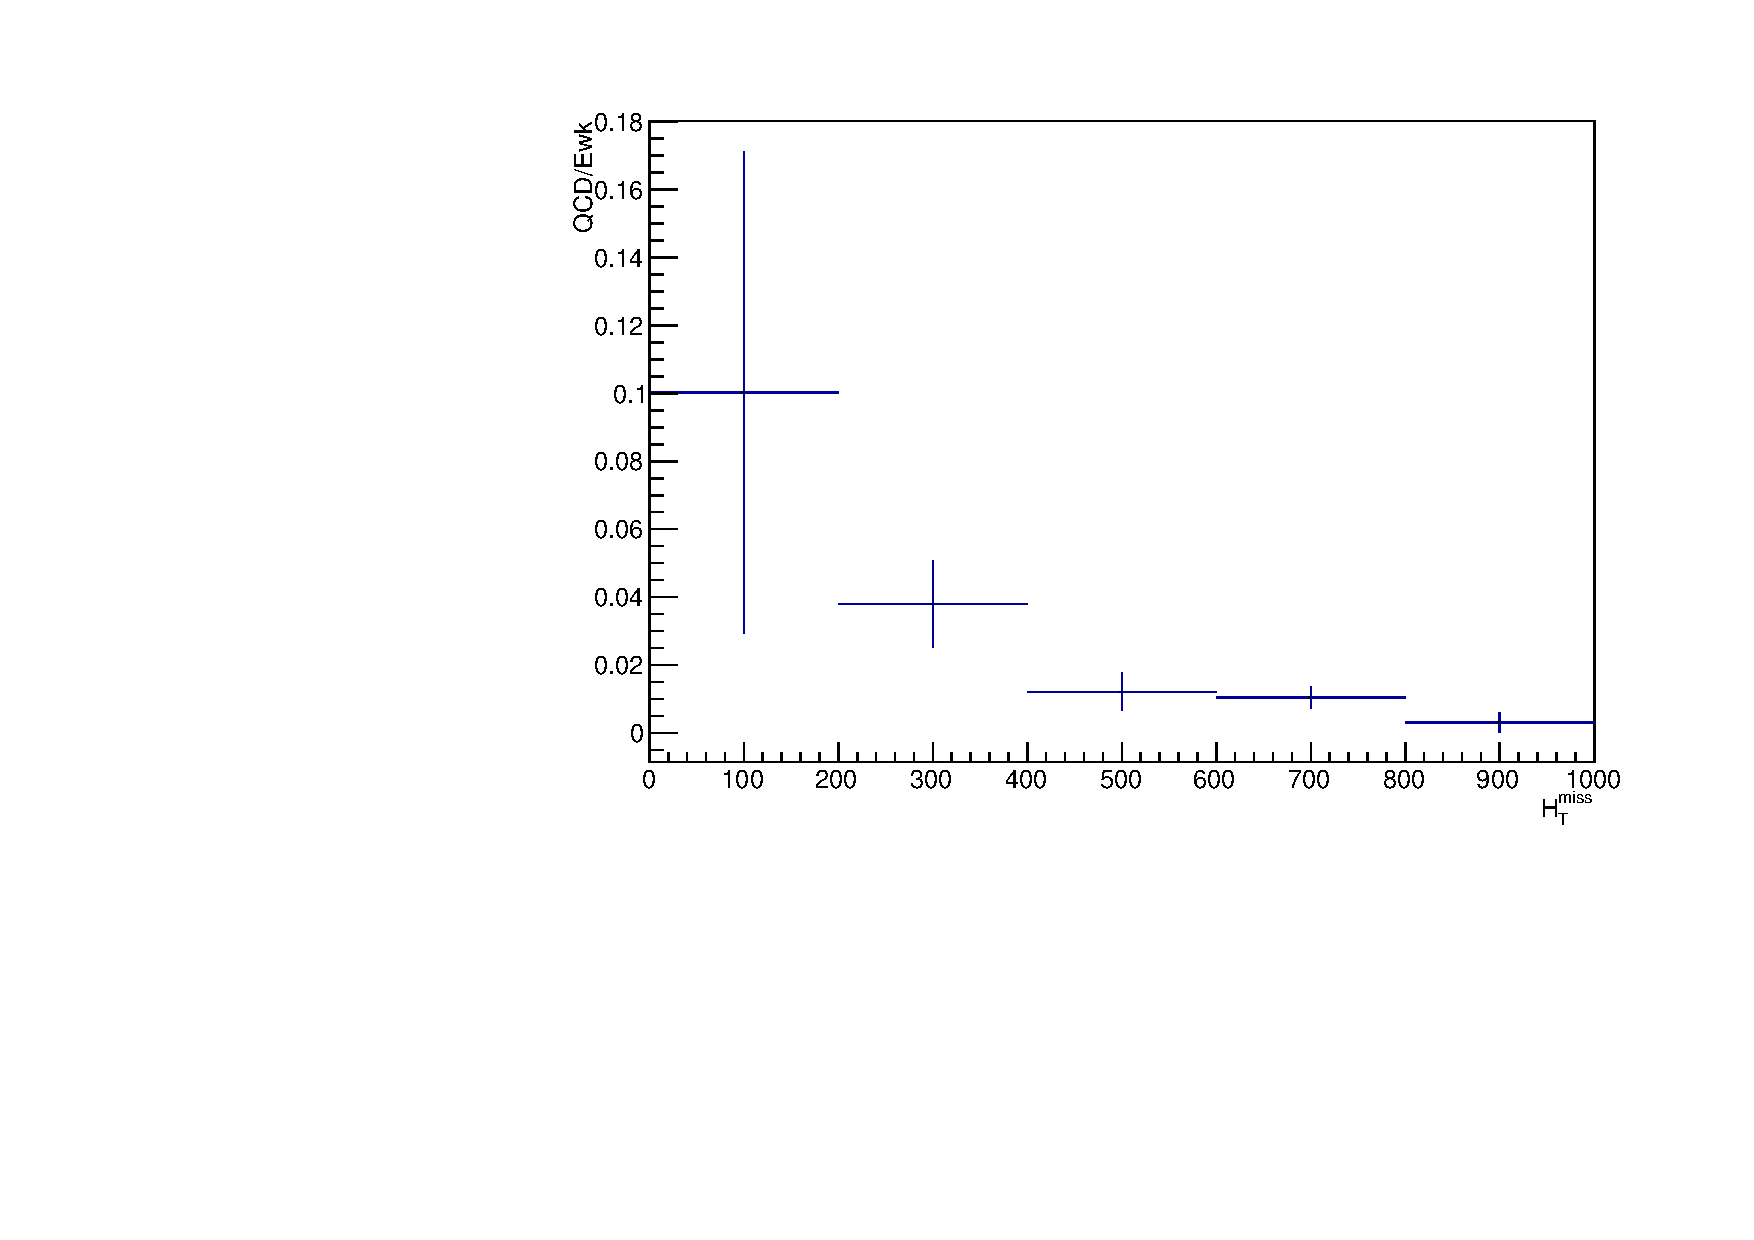
\includegraphics[width=0.5\textwidth]{figures/qcd/plots/mht_ht_ltInfsym}} ~~
%     \subfigure[{ Symmetric,
%     $\scalht>800$~GeV}]{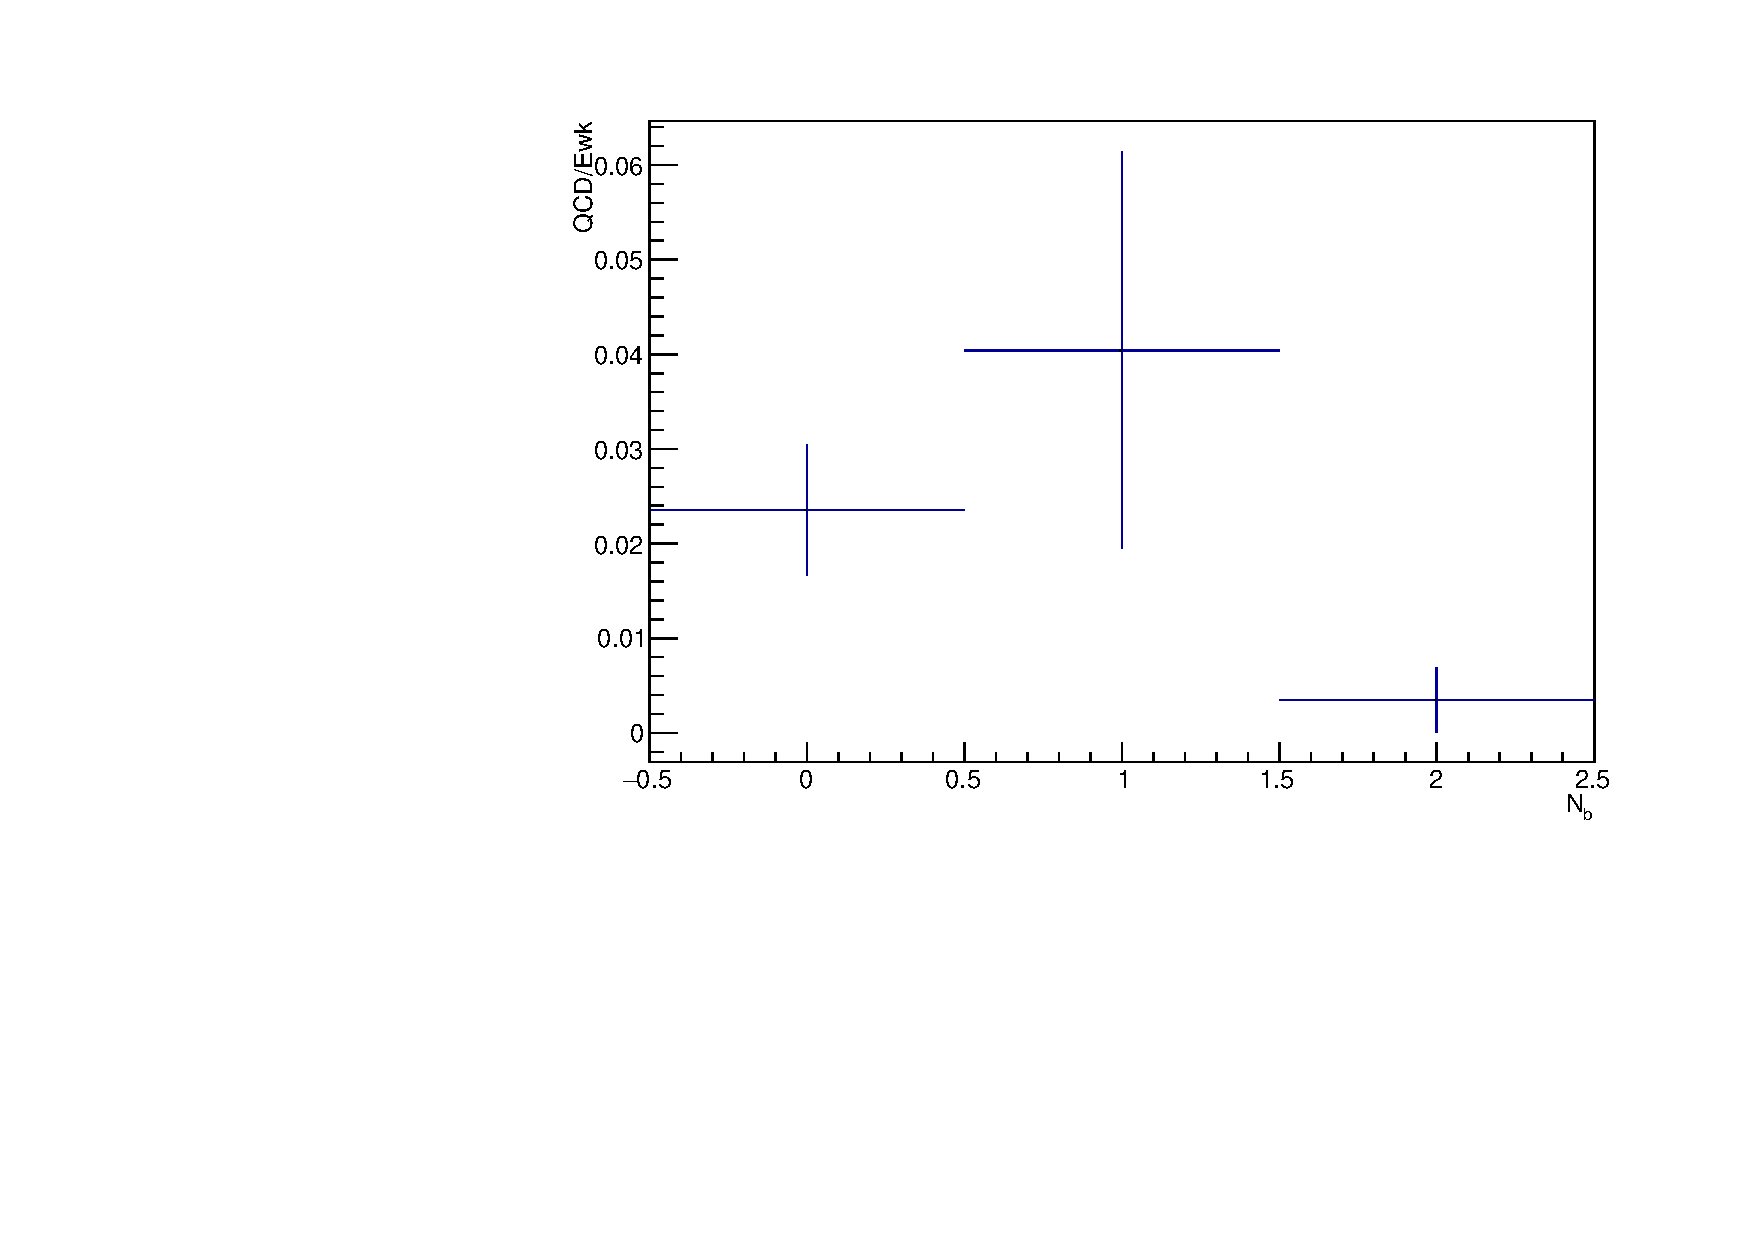
\includegraphics[width=0.5\textwidth]{figures/qcd/plots/nB_ht_ltInfsym}} \\
%       \caption{ Ratio of QCD to EWK Monte Carlo prediction in
%       the signal region for different \scalht selections as a function
%       of \mht (Left) and $\nb$ (Right) for the asymmetric jet
%       category. %A constant fit to the data is represented by the red line, with the $\pm$100\% uncertainty represented by the blue hashed region.
%     }
%     \label{fig:sym_qcd_validation}
%   \end{center} 
% \end{figure}
